% Author Name: José António Portela Areia
% Author Contact: jose.apareia@gmail.com
% Version: 2.2.5 - 2025/03/15
% Public Repository: https://github.com/joseareia/ipleiria-thesis
% Wiki/Getting Help: https://github.com/joseareia/ipleiria-thesis/wiki

%%% Document Options %%%
\documentclass[
    language=english,
    school=agh,
    docstage=final,
    media=paper,
    linkcolor=black,
    chapterstyle=classic,
    coverstyle=classic
]{AGHThesis} % Refer to the Wiki for a list of available options.

%%% Document Version %%%
\DocumentVersion{1.0.0} % This is required only if the 'docstage' is set to 'working'.

%%% Document Metadata %%%
% First Author (Mandatory)
\FirstAuthor{Piotr Urbańczyk}
\FirstAuthorNumber{423649}

% Second Author (Optional)
% \SecondAuthor{Jane Smith}
% \SecondAuthorNumber{2230456}

% Third Author (Optional)
% \ThirdAuthor{July Smith}
% \ThirdAuthorNumber{2230457}

% Supervisor (Mandatory)
\Supervisor{Aleksander Byrski}
\SupervisorMail{olekb@agh.edu.pl}
% Please provide: [Current Title, Affiliation]
\SupervisorTitle{Full Professor, AGH University of Krakow} 

%% Co-Supervisor (Optional)
%\CoSupervisor{Steve Smith}
%\CoSupervisorMail{steve.smith@ipleiria.pt}
%\CoSupervisorTitle{Associate Professor, Polytechnic of Leiria}
%
%% Second Co-Supervisor (Optional)
%\SecCoSupervisor{Shak Smith}
%\SecCoSupervisorMail{shak.smith@ipleiria.pt}
%\SecCoSupervisorTitle{Associate Researcher, Computer Science \& Communication Research Centre}

% Title (Mandatory)
\Title{Multi-Hybrid Swarm Optimization}

% Subtitle (Mandatory)
\Subtitle{Multi-hybrydowa optymalizacja rojowa}

% University (Mandatory)
\University{AGH University of Krakow}

% School (Mandatory)
\School{AGH University of Krakow}

% Department (Mandatory)
\Department{Faculty of Computer Science}

% Degree (Mandatory)
\Degree{Computer Science {\textemdash} Data Science}

% Course (Optional)
% \Course{Offensive \& Defensive Cybersecurity}

% Thesis Theme (Mandatory)
\ThesisType{Master Thesis\\Praca Dyplomowa}

% Local & Date (Mandatory)
\Date{Kraków, \number\year}

% Academic Year 
\AcademicYear{2025/26}

%%% Loading of Glossary and Acronyms %%%
\makeglossaries
\loadglsentries{Matter/04-Glossary}
\loadglsentries[\acronymtype]{Matter/05-Acronyms}


\begin{document}

%%% Front Matter %%%
\ifthenelse{\equal{\CoverOption}{classic}}{
    \newcommand\BackgroundPicCover{%
    \put(0,0){%
    \parbox[b][\paperheight]{\paperwidth}{%
    \vfill
    \centering
    
\includegraphics[width=\paperwidth,height=\paperheight,keepaspectratio]{Figures/Theme/Cover-BG.pdf}% Classic background
    \vfill
    }}}
}
{
    \ifthenelse{\equal{\CoverOption}{dark}}{
        \newcommand\BackgroundPicCover{%
        \put(0,0){%
        \parbox[b][\paperheight]{\paperwidth}{%
        \vfill
        \centering
        
\includegraphics[width=\paperwidth,height=\paperheight,keepaspectratio]{Figures/Theme/Cover-BG-dark.pdf}% Dark background
        \vfill
        }}}
    }{
        \ifthenelse{\equal{\CoverOption}{light}}{
            \newcommand\BackgroundPicCover{%
            \put(0,0){%
            \parbox[b][\paperheight]{\paperwidth}{%
            \vfill
            \centering
            
\includegraphics[width=\paperwidth,height=\paperheight,keepaspectratio]{Figures/Theme/Cover-BG-light.pdf}% Light background
            \vfill
            }}}
        }{}
    }
}

\AddToShipoutPictureBG*{\BackgroundPicCover}

\newgeometry{margin=1.98cm, top=2.15cm, bottom=1.47cm}
\begin{titlepage}
    \latofont
    \ifthenelse{\equal{\CoverOption}{classic}}{
        \color{black} % Classic option: black text
    }{
        \ifthenelse{\equal{\CoverOption}{dark}}{
            \color{white} % Dark option: dark color for text
        }{
            \color{black} % Light option: light color for text
        }
    }
    \vspace*{\baselineskip}
    
    \ifthenelse{\equal{\CoverOption}{classic}}{
        \ifthenelse{\equal{\SchoolOption}{agh}}{
            \begin{figure}
                
\includegraphics[width=0.385\linewidth]{Figures/Theme/Logotypes/AGH_EN_color_cmyk.pdf}
            \end{figure}
        }{}
        
        \ifthenelse{\equal{\SchoolOption}{aghwi}}{
            \begin{figure}
                
\includegraphics[width=0.685\linewidth]{Figures/Theme/Logotypes/AGH_WI_color.pdf}
            \end{figure}
        }{}
    }{
        \ifthenelse{\equal{\CoverOption}{dark}}{
            \ifthenelse{\equal{\SchoolOption}{agh}}{
                \begin{figure}
                    
\includegraphics[width=0.485\linewidth]{Figures/Theme/Logotypes/AGH_EN_W_cmyk.pdf}
                \end{figure}
            }{}
            
            \ifthenelse{\equal{\SchoolOption}{aghwi}}{
                \begin{figure}
                    
\includegraphics[width=0.685\linewidth]{Figures/Theme/Logotypes/AGH_WI_W.pdf}
                \end{figure}
            }{}
        }{
            \ifthenelse{\equal{\CoverOption}{light}}{
                \ifthenelse{\equal{\SchoolOption}{agh}}{
                    \begin{figure}
                        
\includegraphics[width=0.385\linewidth]{Figures/Theme/Logotypes/AGH_EN_B_cmyk.pdf}
                    \end{figure}
                }{}
                
                \ifthenelse{\equal{\SchoolOption}{aghwi}}{
                    \begin{figure}
                        
\includegraphics[width=0.685\linewidth]{Figures/Theme/Logotypes/AGH_WI_B.pdf}
                    \end{figure}
                }{}
            }{}
        }
    }

    \vspace{4.5\baselineskip}

    % Title.
	\noindent
    \makebox[\textwidth][l]{%
        \parbox{\dimexpr\textwidth-4cm\relax}{
            \setstretch{1.03}
            \raggedright\bfseries\fontsize{20}{26}\selectfont\GetTitle
        }
    }

    \vspace{0.8\baselineskip}

    % Subtitle.
    \noindent
    \makebox[\textwidth][l]{%
        \parbox{\dimexpr\textwidth-7cm\relax}{
            \setstretch{1.03}
            \raggedright\fontsize{14}{19}\selectfont\GetSubtitle
        }
    }

    \vspace{35pt}  

    % Author.
    {\noindent\bfseries\fontsize{14}{19}\selectfont\GetFirstAuthor}

    \ifdefined\GetSecondAuthor
        \vspace{8pt}
        {\noindent\bfseries\fontsize{14}{19}\selectfont\GetSecondAuthor}
	\fi

    \ifdefined\GetThirdAuthor
        \vspace{8pt}
        {\noindent\bfseries\fontsize{14}{19}\selectfont\GetThirdAuthor}
	\fi
 
	\vfill

    % School.
	{\noindent\fontsize{10}{12}\selectfont\GetSchool}
	
    % Department.
	{\noindent\fontsize{10}{12}\selectfont\GetDepartment}

    % Degree.
	{\noindent\fontsize{10}{12}\selectfont\GetDegree}

    % Course.
    \ifdefined\GetCourse
        {\noindent\fontsize{10}{12}\selectfont\GetCourse}
	\fi

    \ifthenelse{\equal{\DocStageOption}{working}}{
        \vspace{62pt}
        {\noindent\fontsize{10}{12}\selectfont\overwritecolor{yellow}{\GetDocumentVersion \\ \textit{\today}}} 
        \vspace{62pt}
    }{
        \vspace{100pt}
    }

    % Local & Date.
	{\noindent\fontsize{10}{12}\selectfont\GetDate}

    \vspace{68pt}
\end{titlepage}
\restoregeometry
\MediaOptionLogicBlank
\newcommand\BackgroundPicFrontPage{%
    \put(0,0){%
    \parbox[b][\paperheight]{\paperwidth}{%
    \vfill
    \centering
    
\includegraphics[width=\paperwidth,height=\paperheight,keepaspectratio]{Figures/Theme/Front-Page-BG.pdf}%
    \vfill
}}}
\AddToShipoutPictureBG*{\BackgroundPicFrontPage}

\newgeometry{margin=1.98cm, top=2.15cm, bottom=1.47cm}
\begin{titlepage}
    \latofont
    \color{frontpagedark}
    \vspace*{\baselineskip}

    \ifthenelse{\equal{\SchoolOption}{agh}}{
        \begin{figure}
            
\includegraphics[width=0.385\linewidth]{Figures/Theme/Logotypes/AGH_EN_B_cmyk.pdf}
        \end{figure}
    }
    
    \ifthenelse{\equal{\SchoolOption}{aghwi}}{
        \begin{figure}
            
\includegraphics[width=0.685\linewidth]{Figures/Theme/Logotypes/AGH_WI_B.pdf}
        \end{figure}
    }
    

    \vspace{3\baselineskip}

    % Title.
	\noindent
    \makebox[\textwidth][l]{%
        \parbox{\dimexpr\textwidth-2.5cm\relax}{
            \setstretch{1.03}
            \raggedright\bfseries\fontsize{20}{26}\selectfont\GetTitle
        }
    }

    \vspace{0.8\baselineskip}

    % Subtitle.
    \noindent
    \makebox[\textwidth][l]{%
        \parbox{\dimexpr\textwidth-7cm\relax}{
            \setstretch{1.03}
            \raggedright\fontsize{14}{19}\selectfont\GetSubtitle
        }
    }

    \vspace{35pt}

    % Author.
    {\noindent\bfseries\fontsize{14}{19}\selectfont\GetFirstAuthor}

    \ifdefined\GetSecondAuthor
        \vspace{8pt}
        {\noindent\bfseries\fontsize{14}{19}\selectfont\GetSecondAuthor}
	\fi

    \ifdefined\GetThirdAuthor
        \vspace{8pt}
        {\noindent\bfseries\fontsize{14}{19}\selectfont\GetThirdAuthor}
	\fi

    \vspace{70pt}    

    {
    \noindent
    \latofont
    \fontsize{10}{12}\selectfont
    \renewcommand{\arraystretch}{0.1}
    \hspace*{-2.5pt}\begin{tabular}{@{}r@{\hspace{5pt}}>{\raggedright\arraybackslash}m{6cm}@{}}
        \textbf{Supervisor:} & \GetSupervisor \\ [-.7ex]
        & \setstretch{0.9}{\fontsize{8}{10}\selectfont\itshape \GetSupervisorTitle} \\ [2ex]
        
        \ifdefined\GetCoSupervisor
            \textbf{Co-supervisor:} & \GetCoSupervisor \\ [-.7ex]
            & \setstretch{0.9}{\fontsize{8}{10}\selectfont\itshape \GetCoSupervisorTitle} \\ [.5ex]
        \fi

        \ifdefined\GetSecCoSupervisor        
            & \GetSecCoSupervisor \\ [-.7ex]
            & \setstretch{0.9}{\fontsize{8}{10}\selectfont\itshape \GetSecCoSupervisorTitle} \\
        \fi
    \end{tabular}
    }
    
    \vfill
	
    % School.
	{\noindent\fontsize{10}{12}\selectfont\GetSchool}
	
    % Department.
	{\noindent\fontsize{10}{12}\selectfont\GetDepartment}

    % Degree.
	{\noindent\fontsize{10}{12}\selectfont\GetDegree}

    % Course.
    \ifdefined\GetCourse
        {\noindent\fontsize{10}{12}\selectfont\GetCourse}
	\fi

    \vspace{45pt}

    % Thesis option.
	{\noindent\fontsize{10}{12}\itshape\selectfont\GetThesisType}

    \vspace{35pt}

    % Local and date.
	{\noindent\fontsize{10}{12}\selectfont\GetDate}

    \vspace{68pt}
\end{titlepage}
\restoregeometry
\MediaOptionLogicBlank

%%% Copyright Statement %%%
%\pagenumbering{gobble} % Prevent page numbering.

\vspace*{\fill}

\ifthenelse{\equal{\LanguageOption}{portuguese}}{%
    \noindent \textbf{\GetTitle}
    
    \noindent Copyright \textcopyright~\the\year{} - \GetFirstAuthor, \GetSchool.
    
    \vspace{.575em}
    
    \noindent A presente dissertação é um trabalho original, elaborado exclusivamente para este fim, tendo sido devidamente citados todos os autores cujos estudos contribuíram para a sua elaboração. É permitida a sua reprodução parcial com indicação do autor e referência ao grau, ano letivo, instituição - \textit{Politécnico de Leiria} - e data da defesa pública.
}{%
    \noindent \textbf{\GetTitle}
    
    \noindent Copyright \textcopyright~\the\year{} - \GetFirstAuthor, \GetSchool.
    
    \vspace{.575em}
    
    \noindent This dissertation is original work, written solely for this purpose, and all the authors whose studies and publications contributed to it have been duly cited. Partial reproduction is allowed with acknowledgment of the author and reference to the degree, academic year, institution - \textit{Polytechnic University of Leiria} - and public defense date.
}

\vspace*{\fill}
\MediaOptionLogic

%%% Roman Numeration %%%
\pagenumbering{roman}

%%% Acknowledgements %%%
\ifthenelse{\equal{\LanguageOption}{portuguese}}{%
    \chapter*{Agradecimentos}
}{%
    \chapter*{Acknowledgements}
}

% \guideinfo{In the \textit{Acknowledgment} section, express your gratitude to those who helped and supported your work. Start by thanking your advisors, mentors, or supervisors who provided guidance and expertise. Mention any colleagues, classmates, or team members who contributed to discussions or offered assistance. You can also acknowledge specific organisations, institutions, or funding sources that supported your research or work. Lastly, include any personal acknowledgments for family or friends who offered encouragement and moral support during the project. Keep this section sincere, concise, and professional.}

% The computations were performed on the Ares supercomputer at ACC Cyfronet AGH-UST using the PLGrid Infrastructure.

I gratefully acknowledge Poland's high-performance computing infrastructure PLGrid (ACK Cyfronet AGH) for providing computing resources and support within the computational grant \texttt{plglscclass24}.
The computations were performed on the Ares supercomputer.

\vspace{4cm} % Add vertical space to separate the two "chapters"

% % --- AI Usage Declaration ---
% \ifthenelse{\equal{\LanguageOption}{portuguese}}{%
%     {\raggedleft\Huge \crimsonfont Declaração de Uso de IA \\[1.5em]}
% }{%
%     {\raggedleft\Huge \crimsonfont AI Usage Declaration \\[1.5em]}
% }

\noindent In the preparation of this master’s thesis, AI-powered language tools were employed to enhance the clarity, coherence, and overall quality of the written text. These tools supported tasks such as grammar checking, style adjustments, and phrasing suggestions. Nonetheless, all ideas, research findings, and conclusions are entirely the author’s own. The author accepts full responsibility for any errors or oversights.

\MediaOptionLogicBlank

%%% Abstract %%%
\thispagestyle{plain}
%\chapter*{Resumo}
%
%\guiainfo{Na secção \textit{Resumo}, apresente um resumo conciso do seu projeto, destacando os pontos principais. Comece com uma breve declaração do problema ou objetivo, seguido de uma descrição da sua abordagem ou metodologia. Resuma os principais resultados ou conclusões, salientando a sua importância ou implicações. Conclua com uma ou duas frases sobre a contribuição global ou o impacto do seu trabalho. O resumo deve ser claro e conciso, idealmente com 150-250 palavras, para que os leitores compreendam rapidamente o seu trabalho e a sua importância.}
%
%\keywordspt{Palavra-Chave A, Palavra-Chave B, Palavra-Chave C.}
%
%\MediaOptionLogicBlank

\pdfbookmark[1]{Abstract}{abstract}
\chapter*{Abstract}

% In the \textit{Abstract} section, provide a concise summary of your project, highlighting the key points. Begin with a brief statement of the problem or objective, followed by a description of your approach or methodology. Summarise the main results or findings, emphasising their significance or implications. Conclude with a sentence or two on the overall contribution or impact of your work. Keep the abstract clear and focused, ideally within 150-250 words, to give readers a quick understanding of your research and its importance.

This thesis addresses the premature convergence limitation of Particle Swarm Optimization (PSO), especially in complex, high-dimensional problems. It introduces and evaluates novel informed diversity-enhancing strategies to improve PSO's exploration capabilities. The proposed methodology involves a family of mechanisms based on problem-specific landmarks (best/worst solutions) that apply attraction or repulsion forces within velocity updates. These strategies are categorized into opposing-best (repulsion), attraction-to-worst (negative learning), and opposing-worst (reverse learning) behaviors, forming both single-role algorithms and three multi-hybrid PSO par\-a\-digms: disjoint-role, component-specific, and fully flexible. Rigorous empirical testing on diverse benchmark functions up to 1000 dimensions demonstrates that these strategies, particularly multi-hybrid variants like component-specific Hy\-brid\-Par\-tial\-Dis
-jointPSO, significantly outperform standard PSO and simple perturbation methods in solution quality, convergence, and robustness. Variants employing attraction-to-worst strategies also showed strong, consistent performance. This research establishes that informed, role-based diversity mechanisms are, in most cases, more effective than random perturbations, offering scalable and robust PSO enhancements for complex optimization by better balancing exploration and exploitation.



% \keywordsen{Keyword A, Keyword B, Keyword C.}

\keywordsen{Evolutionary Computation, Swarm Intelligence, Hybrid Metaheuristics, Particle Swarm Optimization (PSO)}


\MediaOptionLogicBlank

%%% Table of Contents, List of Figures and List of Tables %%%
\bookmarktocentry\tableofcontents
\listoffigures
\listoftables
\algorithmstoc
\cleardoublepage

%%% Print: Glossary and Acronyms %%%
\glossarytoc\printnormalglossary
\acronymtoc\printacronymglossary

%%% Arabic Numeration %%%
\cleardoublepage % Ensures main matter starts on an odd page
\pagenumbering{arabic} % Starts page numbering at 1

%%% Chapters %%%
\chapter[Particle Swarm Optimization (PSO)]{\acrfull{pso}}
\label{cp:introduction}

{
% \parindent0pt


\nocite{eberhart1995new}
\acrfull{pso}
% \acrshort{pso} \acrlong{pso}
is 
a meta-heuristic \glslink{metaheuristic} algorithm
% an evolutionary computational model
introduced by \citet{kennedy1995particle} and inspired by the social behavior and synchronous movement of groups of organisms.

\section{%Conceptual
Origins and Motivation}
% The authors of the particle swarm concept identify three primary sources of inspiration.
The development of the particle swarm paradigm was shaped by inspiration from several domains.
Firstly,
the
conceptual
origins of the
model
% particle swarm concept
trace back to early computational simulations aimed at visualizing the coordinated movement of animal formations, such as herds, flocks of birds or schools of fish.
% Particle swarm concept, introduced by \citet{kennedy1995particle},
In referencing early influences on their work, Kennedy and Eberhart point to the simulations of bird flocking developed by \citet{reynolds1987flocks} and by \citet{heppner1990stochastic}. Reynolds, motivated by the aesthetic beauty of 
graceful and erratic choreography of a bird flock,
% flocking behavior,
and Heppner, a zoologist interested in the biological mechanisms behind coordinated group movement, both explored how large numbers of birds could maneuver synchronously---suddenly shifting direction, dispersing, and regrouping with apparent ease. These researchers shared a key insight: that such complex and seemingly unpredictable collective behavior could emerge from simple, local processes,
% and primitive rules,
such as those modeled using systems like cellular automata.
% , provided a conceptual foundation for understanding how decentralized, self-organizing systems might be applied in computational models---an idea central to the development of Particle Swarm Optimization.

Beyond the aesthetic and biological insights, these simulations carried the implicit suggestion that such models could extend to more abstract domains, including human social and cognitive behavior. Drawing on observation that individuals in animal groups can benefit from shared information \parencite{wilson1975sociobiology}, \citeauthor{kennedy1995particle} proposed that similar mechanisms might underlie information exchange and adaptation in human social contexts. Unlike animals constrained by physical proximity and collision avoidance, humans operate in a multidimensional socio-cognitive space, adjusting beliefs, attitudes, and knowledge in response to peers. This abstraction allows for modeling human-like adaptation without the constraints of physical movement.

Within this framework, the PSO algorithm emerged not merely as a visual simulation of flocking, but as a conceptual tool for modeling social learning and adaptation. Particles, conceived as collision-free agents, navigate an abstract solution space, adjusting their positions based on both individual experience and the shared knowledge of the group. Thus, PSO embodies a synthesis of biological modeling, social theory, and computational optimization, grounded in the principle that simple, local rules can drive complex, adaptive behavior.
% in both natural and artificial systems.

Last but not least, in their another seminal paper, \citet{eberhart1995new} highlight that, in addition to the aforementioned artificial life (e-life) methodology, \acrlong{pso} also has its roots in the field of evolutionary computation. Specifically, they note that \acrshort{pso}, on the ground of conceptual foundations, shares important similarities with \acrfull{ga} and \acrfull{es}.

While it was evident from the very beginning that both approaches are similar in their parallel processing nature and share the core principle of population-based search and stochastic exploration, early researchers quickly recognized several important distinctions. Most notably,  \acrshort{ga} and \acrshort{es} employ a ``competitive'' strategy: individuals in the population compete for survival, and poorly performing solutions are replaced by offspring generated through variation operators such as crossover and mutation. In contrast, \acrshort{pso} operates on a ``cooperative'' principle with a velocity-driven update mechanism grounded in behavioral modeling, which allows for smoother, memory-informed trajectories through the search space. A more thorough philosophical and empirical comparison between PSO and GA is provided by \citet{angeline1998evolutionary}.




\section{Algorithm Principles}




% \section{Formal Setup}




In general, the \acrfull{pso} method can be described as:
\begin{equation}\label{eq:pso}
(P', \vec{b}_g') = m(P, \vec{b_g}, f)
\end{equation}
where \(P\) denotes a multiset---referred to as the \textit{swarm}---containing positions in the \gls{search-space}, with each element representing a solution candidate termed \textit{particle}.
% Each particle evaluates the \textit{objective function} \(f\)  at its current location,
% The function \(f\) is the \textit{objective function} used to evaluate each particle,
The function \(f\) is the \textit{objective function} that particles evaluate at their current locations.
The vector \(\vec{b_g}\) denotes the best solution found by the swarm so far, that is, the position corresponding to the lowest (or highest, depending on the optimization goal) value of the objective function \(f\).
In a \(d\)-dimensional \gls{search-space} \(\vec{b_g} = (b_{g}^{1}, b_{g}^{2}, \dots, b_{g}^{d}) \).
The function \(m\)~is a stochastic operator that governs how the swarm evolves, i.e., how particles move within the search space, defined by the equations~\eqref{eq:velocity_update}--\eqref{eq:gbest_update} below.

In line with common practice and terminology borrowed from the field of evolutionary computation, the terms swarm, particles, and objective function are often interchangeably referred to as population, individuals, and fitness function, respectively.

% In a \(d\)-dimensional \gls{search-space},
Each particle is represented by a tuple:
\begin{equation}\label{eq:particle}
X_i = \langle \vec{x_i}, \vec{v_{i}}, \vec{b_i} \rangle,
\end{equation}
where \(\vec{x_i}\) is the particle's position vector, i.e. a set of coordinates describing particle location in \gls{search-space},
% , i.e. a set of coordinates describing a point in space
\(\vec{x_i} = (x_{i}^{1}, x_{i}^{2}, \dots, x_{i}^{d})\). Each particle is also associated with a velocity vector, \(\vec{v_i} =\allowbreak\ (v_{i}^{1}, v_{i}^{2},\dots, v_{i}^{d})\) and retains a personal best position, 
\(\vec{b_i} = (b_{i}^{1}, b_{i}^{2}, \dots, b_{i}^{d}) \).



These terms are used to determine the movement of the particles, which is effectively guided by the following equations:
\begin{equation}\label{eq:velocity_update}
% \forall_{j \in \{ 1,\ldots,d \}}
v_{i}^{j}{}'= \underbrace{\omega v_{i}^{j}}_{\text{inertia}} +
\underbrace{c_1 r_1 (b_{i}^{j} - x_{i}^{j})}_{\text{cognitive component}} +
\underbrace{c_2 r_2 (b_{g}^{j} - x_{i}^{j})}_{\ \ \text{social component}\ \ }
\end{equation}
\begin{equation}\label{eq:position_update}
% \forall_{j \in \{ 1,\ldots,d \}}
x_{i}^{j}{}' = x_{i}^{j} + v_{i}^{j}{}',
\end{equation}
where $\omega$ is the \textit{inertia} weight, \(c_1\) and \(c_2\) are acceleration coefficients (sometimes called \textit{cognitive} and \textit{social} coefficients, respectively), \(r_1\) and \(r_2\) are random values uniformly distributed in the range [0, 1], and the equations are applied to each dimension  $j \in \{ 1,\ldots,d \}$.

The objective function defines a total order over the set of candidate solutions, allowing the algorithm to continuously identify and update the personal and global best positions throughout the search process. Each particle thus keeps track of its own historical best position, and is influenced by the global best position, 
\(\vec{b_g}\), found so far by the entire swarm.
\begin{equation}\label{eq:pbest_update}
\vec{b}_i' =
\begin{cases}
\vec{x}_i', & \text{if } f(\vec{x}_i') < f(\vec{b}_i) \\
\vec{b}_i, & \text{otherwise,}
\end{cases}
\end{equation}
\begin{equation}\label{eq:gbest_update}
\vec{b}_g' = \arg\min_{{\vec{b}_i'}\ \mid\ X_i' \in P'} f(\vec{b}_i').
\end{equation}

% The velocity equation continues the movement in the previous direction and directs a particle's movement toward both its personal best and the global best positions, encouraging convergence to an optimal solution over successive iterations.


The velocity update equation preserves momentum from the previous direction while steering each particle toward its personal best and the global best positions, thereby promoting convergence to the best known solution over successive iterations.

\begin{figure}[H]
    \centering
    \begin{tikzpicture}[
    % scale=1.2,
    point_style/.style={circle, fill=black, inner sep=1.5pt},
    vector_style/.style={-Latex, thick},
    label_style/.style={font=\small},
    component_label_style/.style={font=\footnotesize, sloped, midway},
    guide_line_style/.style={dashed, gray!60, thin}
    ]
    
    % --- Define Coordinates ---
    % Current particle position
    \coordinate (xi_t) at (0,0);
    
    % Personal best and Global best positions
    \coordinate (pbest_i) at (2.2,2.7);
    \coordinate (gbest) at (8,0.5);
    
    % --- Component vectors (as displacements) ---
    \coordinate (inertia_vec) at (0.9, -1.2);
    
    % Cognitive component: c1 * r1 * (p_best,i(t) - x_i(t))
    \coordinate (cognitive_vec_raw) at ($(pbest_i) - (xi_t)$);
    \coordinate (cognitive_vec) at ($1.4*(cognitive_vec_raw)$); % Scaled for visualization
    
    % Social component: c2 * r2 * (g_best(t) - x_i(t))
    \coordinate (social_vec_raw) at ($(gbest) - (xi_t)$);
    \coordinate (social_vec) at ($0.5*(social_vec_raw)$); % Scaled for visualization
    
    % --- Calculate New Velocity and Position ---
    \coordinate (v_tip1) at ($(xi_t) + (inertia_vec) + (cognitive_vec) + (social_vec)$);
    \coordinate (xi_t_plus_1) at (v_tip1); % Since v_i(t+1) is displacement from xi_t
    
    % --- Draw Points and Labels ---
    \node[point_style, label={[label_style]below left:$x_i$}] at (xi_t) {};
    \node[draw, cross out, inner sep=1.5pt, label={[label_style]above:$b_{i}$}] at (pbest_i) {};
    \node[draw, cross out, inner sep=1.5pt, label={[label_style]below right:$b_{g}$}] at (gbest) {};
    \node[circle, fill=black, inner sep=1.5pt, label={[label_style]above right:$x_i'$}] at (xi_t_plus_1) {};
    
    % --- Draw Guide Lines (to pbest and gbest) ---
    \draw[guide_line_style] (xi_t) -- (pbest_i);
    \draw[dash dot, gray!60, thin] (xi_t) -- (gbest);
    
    % --- Draw Resultant New Velocity ---
    \draw[vector_style, ultra thick, opacity=0.5] (xi_t) -- node[component_label_style, below, near end] {${v}_i'$} (v_tip1);
    
    % --- Draw Velocity Components (Tip-to-Tail for clarity) ---
    % 1. Inertia component
    \draw[vector_style, densely dotted] (xi_t) -- node[component_label_style, above] {$\omega v_{i}$} ($(xi_t) + (inertia_vec)$) coordinate (tip_inertia);
    
    % 2. Cognitive component (starting from tip of inertia)
    \draw[vector_style, dashed] (tip_inertia) -- node[component_label_style, above, near end] {$c_1 r_1 (p_{i} - x_{i})$} ($(tip_inertia) + (cognitive_vec)$) coordinate (tip_cognitive);
    
    % 3. Social component (starting from tip of cognitive)
    \draw[vector_style, dash dot] (tip_cognitive) -- node[component_label_style, above] {$c_2 r_2 (p_{g} - x_{i})$} ($(tip_cognitive) + (social_vec)$) coordinate (tip_social);

    \end{tikzpicture}
    \caption[Geometric illustration of PSO's position and velocity update]{Geometric 2-dimensional illustration of a single particle's position and velocity update in PSO.}
    \label{fig:PSO_geometric_illustration}
\end{figure}


% Naturally,
% \begin{equation}\label{eq:pbest_update}
% \vec{b}_i' =
% \begin{cases}
% \vec{x}_i', & \text{if } f(\vec{x}_i') < f(\vec{b}_i) \\
% \vec{b}_i, & \text{otherwise,}
% \end{cases}
% \end{equation}
% \begin{equation}\label{eq:gbest_update}
% \vec{b}_g' = \arg\min_{{\vec{b}_i'}\ \mid\ X_i' \in P'} f(\vec{b}_i').
% \end{equation}

% These equations encode the core intuition behind PSO: particles are agents that "learn" from their own successes (personal experience) and from the collective experience of the swarm. The inertia term maintains momentum from previous movements, which helps the swarm explore broadly. The cognitive component pulls particles back toward regions where they individually performed well, while the social component biases them toward globally successful areas. By dynamically balancing these influences through stochastic variation, PSO achieves a trade-off between exploration and exploitation---a hallmark of effective metaheuristic design.


The algorithm begins by initializing a population of particles, each representing a candidate solution, randomly sampled within the defined bounds of the \gls{search-space}. In parallel, initial velocity vectors are randomly assigned to each particle. The fitness of each particle is then evaluated using the objective function, allowing the assignment of each particle's personal best position. The best-performing particle among the entire swarm establishes the initial global best position.

Following initialization, the swarm enters an iterative optimization loop. In each iteration, particle velocities and positions are updated according to the above-mentioned equations \eqref{eq:velocity_update} and \eqref{eq:position_update}. After the movement step, each particle's new position is evaluated, and personal and global bests are updated if improvements are observed.


This iterative process---of evaluating fitness, updating velocities and positions, and tracking and adjusting towards the best solutions---continues until a predefined termination criterion is met.
Upon completion, the global best position discovered by any particle during the process is returned as the algorithm's final solution.

\vspace{.935em}

\begin{algorithm}[H]
% \caption{Particle Swarm Optimization (PSO)}
\caption{PSO}
\KwIn{Swarm size \(N\), acceleration coefficients \(c_1\) and \(c_2\), inertia weight \(\omega\)}
\KwOut{Best solution found}
Initialize population of \(N\) particles with random positions and velocities\;
Evaluate the fitness of each particle\;
Set global best position \(b_g\), for each particle set personal best position \(b_i\)\;
    \While{Termination criterion is not met}{
        Modify each particle's position and velocity by equations (\ref{eq:velocity_update}) and (\ref{eq:position_update})\;
        Evaluate the fitness of each particle\;
        Update the personal best \(b_i\) and global best \(b_g\) positions if necessary\;        
    }
\Return The global best position \(b_g\) as the final solution\;
\end{algorithm}

\vspace{.935em}

At its core, \acrshort{pso} mimics the social dynamics of a group of entities or agents---i.e., particles---that explore a solution space collectively, adjusting their paths based on individual experience and shared knowledge within the swarm. 

\section{Key Components and Parameters}

- velocity components (and coefficients)
- termination criterion
- repair algorithm (bounce, clip, reinitialize)
- early variants (Local Best PSO)


\section{Possible Application}

PSO offers elegant yet powerful approach to solving complex \glspl{optimization-problem}.

\section{Pros and Cons}
Welcome to the \textcolor{maincolor}{\textit{IPLeiria Thesis}} template! Thank you for choosing it for your dissertation, reports, or other projects. This template reflects countless hours of development and learning, and I hope you enjoy using it as much as I enjoyed creating it. This chapter introduces the motivation behind the template and guides you through the initial steps to start using it. In \autoref{cp:user-guide}, you will find a comprehensive guide to fully utilise the template, and \autoref{cp:latex-tutorial} provides a concise \LaTeX~tutorial to help you maximise its capabilities. Happy reading and future writing!

%%%%%%%%%%%%%%%%%%%%%
I've known \LaTeX~since 2020, and since then, I have been using it constantly for a wide variety of purposes. Over time, I've used and reviewed more than a hundred templates, and there is always something missing. \textit{Always}. If a template is powerful -- \textit{i.e.}, it has many options and is highly customisable -- it's often not well-organised. Conversely, if it is well-organised, it usually lacks flexibility and customisation options. Some templates even compile with numerous errors and warnings. Most importantly, the majority are not very user-friendly. For these reasons, I decided to create my own template for theses and reports, specifically tailored for the Polytechnic University of Leiria. Throughout this project, I focused on achieving four key goals: \(i)\) creating a template that is organised and well-structured in terms of file organisation, \(ii)\) ensuring it is clean yet aesthetically pleasing and professional, \(iii)\) making it customisable to suit different needs, and \(iv)\) designing it to be user-friendly, especially for newcomers.

\section{Getting Started}
To start using this template, you first need to know how to use \LaTeX. For this, please refer to \autoref{cp:latex-tutorial}. Once you are familiar with \LaTeX, you will need to either install it locally or use an online \LaTeX~editor.

If you prefer an online editor, I highly recommend \href{https://www.overleaf.com/}{Overleaf}. While Overleaf offers a paid subscription for extended compilation time, this template is specifically designed to compile within the limits of the free subscription plan. To use the template in Overleaf, just refer to \href{https://www.overleaf.com/latex/templates/unofficial-polytechnic-university-of-leiria-estg-thesis-slash-report-template/tqgbrncfhwgt}{official template page} and click \textit{Use as Template}. But if you prefer to use a different version of it (which I do not recommend), you can do the following:

\begin{enumerate}[font=\itshape]
    \setlength{\itemsep}{.375em}
    \item \textit{Download the \href{https://github.com/joseareia/ipleiria-thesis/releases}{desired version} from the GitHub repository as a Zip file.}
    \item \textit{Login to your Overleaf account.}
    \item \textit{In your Project area, click in the menu and then: New Project \(\to\) Upload Project.}
    \item \textit{Upload the Zip file.}
    \item \textit{Let Overleaf compile the document.}
\end{enumerate}

If you choose to use a local editor, you must first install \LaTeX~on your machine. For this, there are several options, but I personally recommend either \href{https://www.tug.org/texlive/}{TeX-Live} or \href{https://miktex.org/}{MikTeX}. After installing \LaTeX, you will need to select an editor for writing and editing your documents. To help with this decision, I suggest checking out this helpful \href{https://tex.stackexchange.com/questions/339/latex-editors-ides}{post}, which provides a comprehensive overview of various editors you can use. Once \LaTeX~and your editor are set up, simply clone or download the \href{https://github.com/joseareia/ipleiria-thesis/releases}{latest} version of the template from GitHub and start using it!

\begin{block}[tip]
\textit{Within the official GitHub repository, you will find a \href{https://github.com/joseareia/ipleiria-thesis/blob/master/Makefile}{Makefile} and a \href{https://github.com/joseareia/ipleiria-thesis/blob/master/.latexmkrc}{Latexmk} configuration file, both of which can be used to compile this project. The Makefile utilises \texttt{rubber} as the compiler and has a dependency of \texttt{inotify-tools}. Feel free to use whichever option best suits your needs.}
\end{block}

\section{Getting Help}
As a newcomer, you may encounter situations where you want to do something in \LaTeX~or with this template but aren't sure how. When questions arise, you have several options. First, you can read the wiki available in the \href{https://github.com/joseareia/ipleiria-thesis}{GitHub} repository for this template. Another great option is the \href{https://tex.stackexchange.com/}{TeX Stack Exchange}, an active community that can help with nearly any issue. Of course, Google is always a reliable resource. If all else fails, feel free to contact me directly with any questions about the template. You can reach me at \textit{\textcolor{blue}{\myuline{jose.apareia@gmail.com}}}.

\subsection{Issues, Feature Request and Suggestions}
If, by any chance, you encounter a bug, have a suggestion, or would like to request a feature, you can submit them via the \textit{Issues} tab in the \href{https://github.com/joseareia/ipleiria-thesis}{GitHub} repository. Please be as descriptive as possible when reporting issues, and make sure to provide the appropriate labels to help me triage them effectively.

For feature requests or suggestions, you can either follow the steps mentioned above or, if you prefer, you can implement the feature yourself and submit a pull request. Both pull requests and pushes trigger a \href{https://github.com/joseareia/ipleiria-thesis/actions/workflows/latex.yml}{GitHub Action} that will automatically compile the document. If the compilation fails, the pull request will be automatically rejected. Please keep this in mind and take care when submitting changes.

\subsection{In-Built Comments, Guidance Texts and Warnings}
Within this document template, you may encounter informational text displaying the message ``Writing Guidance.'' These sections are provided solely as guidance to help users understand what content should be included in specific sections. They are not related to the \LaTeX~code itself within this template.

While navigating through the template, especially the configuration files, you will notice that everything is thoroughly commented. \LaTeX~can sometimes be difficult to understand without proper documentation for the packages we are working with. With that in mind, I have made an effort to comment on all the changes I've made. Occasionally, I may forget or deem it unnecessary to comment on simpler changes, but more advanced modifications are always accompanied by detailed comments.

Finally, regarding warnings: please take them into consideration when compiling the document. As you may have noticed, the template is designed to be free of warnings, so please strive to maintain this clean compilation.

\section{Important Notices}
Although this template is specifically tailored for students from all six schools of the Polytechnic University of Leiria, you are welcome to use it if you are from a different institution. It is highly customisable and can be easily modified to suit the needs of other schools. If your school is interested in adopting this as the official template, please contact me first. 

If you decide to use this template, please consider acknowledging it in your work. To do so, simply cite it using \verb|\citep{IPLeiriaThesis}|. You can also show your appreciation for this template by giving a \href{https://github.com/joseareia/ipleiria-thesis/stargazers}{star} on the GitHub repository. This helps increase its visibility, and you will receive notifications about the latest updates and releases. Either way, acknowledging this work, which involved significant effort and countless hours, would be greatly appreciated.




}
\cleardoublepage
\chapter[Comprehensive User Guide: Instructions for Using the Template]{Comprehensive User Guide Instructions for Using the Template}
\label{cp:user-guide}

{
\parindent0pt

If you plan to use this template, please read this chapter carefully. It provides all the information you need to effectively use the template, including the mandatory modifications (\textit{e.g.}, title, subtitle, author information) and other configurations that, while not highly recommended, are optional. The template comprises various directories and files, including a total of seven distinct directories and dozens of files. Among these, the most important are \texttt{IPLeiriaMain.tex} and \texttt{IPLeiriaThesis.cls}. Below, \autoref{tab:file-structure} presents the different directories available, along with their descriptions and a check-mark indicating whether you need to access the directory to make changes. Of course, the check-mark indicates that you can make changes to the content, while a hyphen signifies that you should not modify it.

\begin{table}[!htpb]
    \setlength{\extrarowheight}{2pt}
    \caption[Directory structure and file organisation]{Overview of the directory structure in this template.}
    \label{tab:file-structure}
    \begin{tabularx}{\textwidth}{lcX}
        \toprule
        \\[-1.5\normalbaselineskip]
        \textbf{Directory} & \textbf{Modifiable} & \textbf{Description} \\ [0em]
        \midrule
        \textit{Bibliography} & $\checkmark$ & This folder contains the bibliography file used to manage references throughout the document. \\
        \textit{Chapters} & $\checkmark$ & Individual chapters of the thesis are organised in this directory, making it easy to work on sections separately. \\
        \textit{Code} & $\checkmark$ & Code examples and relevant scripts are stored here, supporting the content of the thesis. \\
        \textit{Configurations} & - & All configuration files required for the template, such as layout and style settings, are placed in this directory. \\
        \textit{Figures} & $\checkmark$ & All figures and images referenced within the document are stored in this folder for easy access and management. \\
        \textit{Matter} & - & The front matter of the document, including the cover page, copyright statement, and glossary, is assembled in this directory. \\
        \textit{Metadata} & $\checkmark$ & This folder holds the metadata file, where key document details such as the author, title, and supervisor can be customised. \\
        \bottomrule
    \end{tabularx}
\end{table}

It is crucial to note that the files are organized according to a specific naming convention, which must be \textbf{respected} and \textbf{maintained}. The naming convention consists of an ascending two-digit numeric value, followed by a hyphen, and then the file name in capital letters. The name should always aim to be a single word. If more than one word is necessary, they should be separated by a hyphen and capitalised.

% \begin{verbatim}
% 00-Abstract.tex
% 01-Introduction.tex
% 02-User-Guide.tex
% ...
% \end{verbatim}

\begin{block}[note]
\textit{While \autoref{tab:file-structure} indicates that the \textit{Matter} directory is not modifiable, two files within that directory should be altered when necessary: \texttt{04-Glossary.tex} and \texttt{05-Acronyms.tex}. Although the names are fairly self-explanatory, these files should contain the glossary and acronyms entries, respectively.}
\end{block}

The two files mentioned earlier, \texttt{IPLeiriaMain.tex} and \texttt{IPLeiriaThesis.cls}, should be used with caution. The main file, as the name suggests, is the master file where you will add the necessary chapters to be included in your work. The class file, on the other hand, requires even more caution, and it is not recommended to alter it.

\section{Template and Class Options}
\label{sec:class-options}
The first thing you need to do is specify the options within the \texttt{IPLeiriaMain.tex} file. How do you do that? It's simple. On the very first line, you will find a \texttt{documentclass} command that loads the custom class for this template. In this call, you can pass the options you need. The available options, presented in a key-argument style, are listed in \autoref{tab:template-options}.

{
\setlength{\extrarowheight}{-1.75pt}
\begin{xltabular}{\textwidth}{lX}
\caption{Class options supported by the template.}
\label{tab:template-options} \\
%
\toprule 
\multicolumn{1}{l}{\textbf{Options}} & \multicolumn{1}{l}{\textbf{Description}} \\ 
\midrule
\endfirsthead
%
\multicolumn{2}{c}%
{{\textit{\bfseries Table \thetable\ continued from previous page.}}} \\
%
\toprule 
\multicolumn{1}{l}{\textbf{Options}} & \multicolumn{1}{l}{\textbf{Description}} \\ 
\midrule
\endhead
%
\bottomrule
\addlinespace[1mm]
\multicolumn{2}{r}%
{{\textit{Continued on the next page.}}} \\
\endfoot
\bottomrule
\endlastfoot

\textbf{school=OPT} & \textbf{Choosing a school and its corresponding logo.} \\
\multirow[t]{2}{*}{\footnotesize{\textit{estg, esecs, esslei, esad, estm}}} & \footnotesize{\textit{$\Rightarrow$ Default: school=estg}} \\
& \footnotesize{\textit{This option only modifies the school name and the corresponding logo, which will be displayed on the cover and front page.}} \\[1.70em]

\textbf{language=OPT} & \textbf{Language preference selection.} \\
\footnotesize{\textit{portuguese, english}} & \footnotesize{\textit{$\Rightarrow$ Default: language=english}} \\[0.85em]
        
\textbf{chapterstyle=OPT} & \textbf{Selection of a cover design style.} \\
\multirow[t]{2}{*}{\footnotesize{\textit{classic, modern, fancy}}} & \footnotesize{\textit{$\Rightarrow$ Default: chapterstyle=classic}} \\
& \footnotesize{\textit{This option modifies the appearance of the chapter, including its title and numbering style. Explore the available styles and apply the one you prefer.}} \\[1.70em]

\textbf{coverstyle=OPT} & \textbf{Choosing a style for the chapter.} \\
\multirow[t]{3}{*}{\footnotesize{\textit{classic, bw}}} & \footnotesize{\textit{$\Rightarrow$ Default: coverstyle=classic}} \\
& \footnotesize{\textit{classic $\rightarrow$ Put the cover on in the original red.}} \\
& \footnotesize{\textit{bw $\rightarrow$ Make the cover black and white.}} \\

\pagebreak

\textbf{docstage=OPT} & \textbf{Choosing a stage for you document.} \\
\multirow[t]{3}{*}{\footnotesize{\textit{final, working}}} & \footnotesize{\textit{$\Rightarrow$ Default: docstage=final}} \\
& \footnotesize{\textit{final $\rightarrow$ Assumes this is the final version of the document.}} \\
& \footnotesize{\textit{working $\rightarrow$ It assumes the document is a work in progress.}} \\[.3em]

\textbf{media=OPT} & \textbf{Project media type.} \\
\multirow[t]{3}{*}{\footnotesize{\textit{paper, screen}}} & \footnotesize{\textit{$\Rightarrow$ Default: media=paper}} \\
& \footnotesize{\textit{paper $\rightarrow$ Blank pages will appear between sections.}} \\
& \footnotesize{\textit{screen $\rightarrow$ Blank pages will not appear between sections.}} \\[.3em]

\textbf{colorlink=OPT} & \textbf{Main theme color.} \\
\multirow[t]{2}{*}{\footnotesize{\textit{color}}} & \footnotesize{\textit{$\Rightarrow$ Default: colorlink=black}} \\
& \footnotesize{\textit{This option requires a valid color name. Refer to the xcolor manual (subsection 4.2) to select a valid color.}} \\
\end{xltabular}
}

\begin{block}[tip]
\textit{Although the default option for \texttt{linkcolor} is \texttt{black}, it is highly advisable to use \texttt{red!45!black} instead. The same applies to \texttt{coverstyle}, for which it is preferred to use the \texttt{classic} option.}
\end{block}

% \begin{block}[warning]
% \textit{If any option or argument is passed and it does not exist, an error or a warning will be raised, respectively. Please pay attention to warnings and strive to keep the template and/or your document free of warnings.}
% \end{block}

After setting the options within the main class, you're ready to proceed with the metadata customisation. How can you do that? Please refer to \autoref{sec:metadata}.

\section{Metadata Customisation}
\label{sec:metadata}
While options like language and school can be passed as arguments to the main class, other options, such as author and title, need to be defined manually. Since this template supports a wide range of metadata options, a dedicated file is provided for this purpose. The file is located at \texttt{Metadata/Metadata.tex} and contains the metadata variables you can modify, along with comments explaining each variable and whether it is mandatory for the document. To omit a variable, simply comment it out. Below, \autoref{tab:metadata} presents all the available metadata variables, their GET command, and whether they are mandatory. The GET command is important if you want to automatically retrieve the name or information stored in a given variable.

\begin{longtable}[c]{llc}
\caption{Metadata variables within the template.}
\label{tab:metadata} \\
\toprule
\textbf{Variable} & \textbf{Macro Commands} & \textbf{Mandatory} \\ \midrule
\endfirsthead
%
\multicolumn{3}{c}%
{{\textit{\bfseries Table \thetable\ continued from previous page.}}} \\
%
\toprule
\textbf{Variable} & \textbf{Macro Commands} & \textbf{Mandatory} \\ \midrule
\endhead
%
\bottomrule
%
\addlinespace[1mm]
\multicolumn{3}{r}%
{{\textit{Continued on the next page.}}} \\
\endfoot
%
\bottomrule
%
\endlastfoot
%
Title            & \verb|\GetTitle|         & $\checkmark$ \\
Subtitle         & \verb|\GetSubtitle|      & $\checkmark$ \\
University       & \verb|\GetUniversity|    & $\checkmark$ \\
School           & \verb|\GetSchool|        & $\checkmark$ \\
Department       & \verb|\GetDepartment|    & $\checkmark$ \\
Degree           & \verb|\GetDegree|        & $\checkmark$ \\
Course           & \verb|\GetCourse|        & -            \\
Local and date   & \verb|\GetDate|          & $\checkmark$  \\ 
Academic year    & \verb|\GetAcademicYear|  & $\checkmark$ \\ 

Thesis type (\scriptsize{\textit{Dissertation, Project or Internship}}) & \verb|\GetThesisType| & $\checkmark$ \\

First author name           & \verb|\GetFirstAuthor|        & $\checkmark$ \\
First author identification & \verb|\GetFirstAuthorNumber|  & $\checkmark$ \\ 

Second author name           & \verb|\GetSecondAuthor|          & - \\
Second author identification & \verb|\GetSecondAuthorNumber|    & - \\ 

Third author name           & \verb|\GetThirdAuthor|        & - \\
Third author identification & \verb|\GetThirdAuthorNumber|  & - \\ 

Supervisor name                  & \verb|\GetSupervisor|        & $\checkmark$ \\
Supervisor e-mail                & \verb|\GetSupervisorMail|    & $\checkmark$ \\
Supervisor title and affiliation & \verb|\GetSupervisorTitle|   & $\checkmark$ \\ 

Co-supervisor name                  & \verb|\GetCoSupervisor|       & - \\
Co-supervisor e-mail                & \verb|\GetCoSupervisorMail|   & - \\
Co-supervisor title and affiliation & \verb|\GetCoSupervisorTitle|  & - \\ 

Second co-supervisor name                   & \verb|\GetSecCoSupervisor|      & - \\
Second co-supervisor e-mail                 & \verb|\GetSecCoSupervisorMail|  & - \\
Second co-supervisor title and affiliation  & \verb|\GetSecCoSupervisorTitle| & - \\
\end{longtable}

If, by any chance, \textbf{you want to add more options}, please contact me by opening an issue in the official GitHub repository or via the email provided in this document.

\section{Custom Commands}
Within this template, some custom commands are also available for your use. For example, if you are writing your thesis and want to add a to-do note, you can easily insert a block with the option \verb|todo|, as follows: \verb|\begin{block}[todo]|. This will insert a to-do block with a style similar to Markdown. Other available options are: \verb|tip|, \verb|warning|, and \verb|note|. Below is a visual example for each one.

\vspace{.875em}
\begin{tcbraster}[
    raster columns=2, 
    raster equal height, 
    nobeforeafter, 
    raster column skip=2cm
]
\begin{block}[todo]
    \textit{This is a to-do block.}
\end{block}
\begin{block}[tip]
    \textit{This is a tip block.}
\end{block}
\end{tcbraster}

\begin{tcbraster}[
    raster columns=2, 
    raster equal height, 
    nobeforeafter, 
    raster column skip=2cm
]
\begin{block}[warning]
    \textit{This is a warning block.}
\end{block}
\begin{block}[note]
    \textit{This is a note block.}
\end{block}
\end{tcbraster}
\vspace{.875em}

\begin{block}[coco]
    \textit{This is a coco block.}\\
    DWa traa\\
    sfs asefsg srg jj.
\end{block}

Another custom command that can come in handy is \verb|\myuline{TEXT}|, which creates a visually improved underline. The default \LaTeX~underline is not ideal because it sits directly below the bottom margin of the word, increasing the line height of the paragraph. This new command provides a \myuline{better} and more \myuline{stylish} underline.

\section{Custom Chapter Insertion}
As stated before, to use this template, you need to do three things: set the appropriate options in the document class (refer to \autoref{sec:class-options}), update the document metadata (refer to \autoref{sec:metadata}), and create and import your custom chapters. To create and import a custom chapter, follow these steps: \(i\) create a TeX file under the Chapters directory that follows the predefined naming convention, and \(ii)\) include it in the main file using the command \verb|\include{CHAPTER}|. And voilà, your first chapter is ready!
}
\cleardoublepage
\chapter[Experiment]{Experiment}
\label{cp:experiment}

{
\parindent0pt

In this chapter, we will introduce the \LaTeX~working environment, highlighting the basic essentials you will need to produce your thesis. First of all, \LaTeX~(pronounced ``LAY-tek'' or ``LAH-tek'') is a tool for creating professional-quality documents. Unlike \textit{What You See Is What You Get} editors like Microsoft Word, \LaTeX~uses plain text files containing both content and formatting commands. These files are processed by a TeX engine, which interprets the commands to produce a polished, typeset PDF. This approach lets you focus on your content, leaving the precise formatting and layout to \LaTeX~and the TeX engine, ensuring a professional result every time. While this chapter will introduce you to some important functionalities of \LaTeX~, please take the time to learn \LaTeX~from the beginning. You can always refer to the Overleaf \href{https://www.overleaf.com/learn/latex/Learn_LaTeX_in_30_minutes}{Learn LaTeX} series for guidance.

% Moreover, if you are spending an enormous amount of time writing your thesis, it's better to use a proper tool where you don't need to worry about professional layout but can focus solely on the content.

\section{Citations}
\label{sec:citations}
We present two distinct approaches for citing entries in the bibliography. The first method involves in-text citations, executed using \verb|\citet{ENTRY}|, while the second method employs \verb|\citep{ENTRY}| for citations within a paragraph. Below is an example demonstrating both usages. It's essential to note that you can cite multiple works within the same citation environment. To achieve this, you should use the following format: \verb|\citep{ENTRY1, ENTRY2, ...}|. It is also possible to cite only the title of the work or the author of the same. To do this, please use \verb|\citetitle{ENTRY}| for title citations and \verb|\citeauthor{ENTRY}| for author citations.

\begin{block}[tip]
\textit{Proper citations play a crucial role in academic writing, serving as the foundation for credibility, transparency, and the advancement of knowledge. They are a fundamental aspect of responsible scholarly writing. Please ensure accurate and appropriate citations.}
\end{block}

\noindent\textbf{Example:} A novel signature scheme is introduced, along with an implementation of the Diffie-Hellman key distribution scheme that accomplishes a public key cryptosystem \citep{kennedy1995particle}. According to \citet{kennedy1995particle}, a new signature scheme that accomplishes a public key cryptosystem is introduced (...) This template was created by \citeauthor{kennedy1995particle}, with the title \citetitle{kennedy1995particle}.

\section{References}
Much like citations, it is advisable to employ references in your document for citing crucial elements such as chapters, sections, figures, or tables. To reference these elements, begin by creating a label. This label can be generated using \verb|\label{TEXT}|, and it should be positioned within the element you intend to refer to. Once the element is created, you can utilise \verb|\ref{LABEL}| to generate an in-text reference. \textbf{We strongly recommend using} \verb|\autoref{LABEL}|. This command automatically creates a custom link with color corresponding to the type of element being referred to. For instance, a chapter reference will appear like this: \autoref{cp:introduction}, rather than simply Chapter \ref{cp:introduction}. 

\begin{block}[tip]
\textit{Properly referencing elements within the document, such as \textbf{chapters, sections, figures, tables, or listings}, is crucial.}
\end{block}

\section{Glossary and Acronyms}
The document includes both a glossary and an acronym list, accessible at the beginning of the document. You can create a new entry in either the \verb|Matter/02-Glossary| or \verb|Matter/03-Acronyms| sections\gls{optimization-problem}, depending on the type of entry you intend to add. Once the entry is created, you can reference it using \verb|\gls{ENTRY}| for glossary entries. For acronym entries, there are two ways to reference them. The first method, \verb|\acrfull{ENTRY}|, should be used the first time the acronym appears in the text as it automatically provides the definition in-text. Subsequently, to refer to the acronym without repeating its meaning, use \verb|\acrshort{ENTRY}|.

\vspace{.875em}
\textbf{Example:} Utilising \Gls{search-space} for \Gls{optimization-problem} is essential. It is advisable to seek both the \acrfull{pso} and \acrfull{ga} because of this. Subsequently, with the aid of \acrshort{pso} and \acrshort{ga}, we can do.

\section{Figures}
In \LaTeX, integrating figures is a straightforward process. To insert them, you should utilise the environment \verb|\begin{figure}|. You can customise the \verb|width| parameter according to your requirements, but it is crucial to select a high-quality figure when inserting it into your documents. It is equally crucial to furnish a well-crafted caption. If necessary, consider including citations or references to indicate the figure's origin. The caption environment is denoted as \verb|\caption{TEXT}|. To generate a smaller caption for the Table of Figures, be sure to utilise the format \verb|\caption[SMALL_TEXT]{BIG_TEXT}|. By following the aforementioned tips, we can create a figure as demonstrated in \autoref{fig:figure-01}.

\begin{figure}[!htpb]
    \centering
    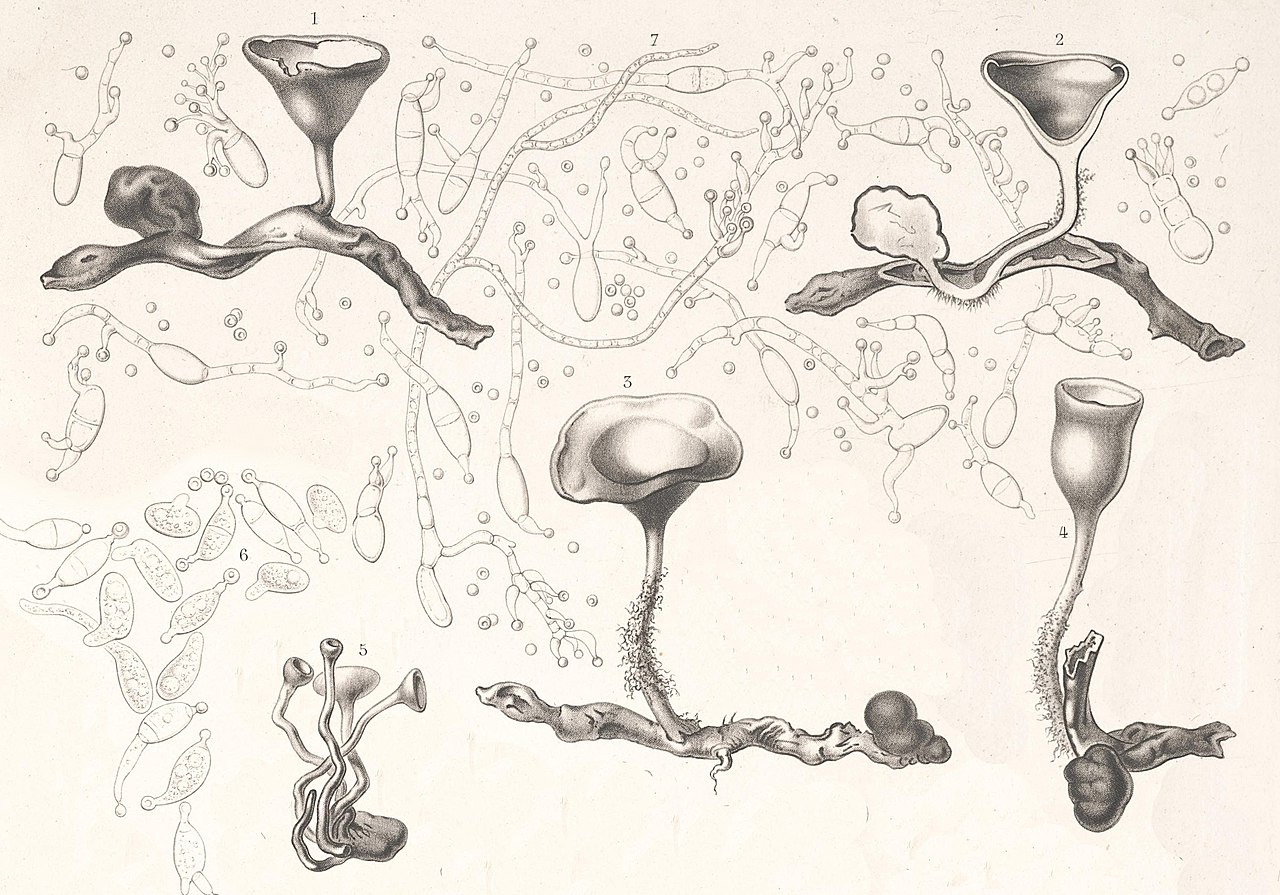
\includegraphics[width=\linewidth]{Figures/PezizaTuberosa.jpg}
    \caption[Illustration of the fungus Dumontinia tuberosa.]{Illustration of the fungus Dumontinia tuberosa by physician, mycologist, and illustrator Charles Tulasne (1816–1884) in the book Selecta Fungorum Carpologia (1861–65). (Name of the original work: Peziza tuberosa parasite on Anemone nemorosa).}
    \label{fig:figure-01}
\end{figure}

For the purpose of comparing or for other reasons, you can insert side-by-side figures using both the \verb|\begin{figure}| and \verb|\begin{subfigure}| environments. You can also refer to the sub-figure as \autoref{fig:figure-02.1} and \autoref{fig:figure-02.2}.

\begin{figure}[!htpb]
    \centering
    \begin{subfigure}{0.45\textwidth}
        \centering
        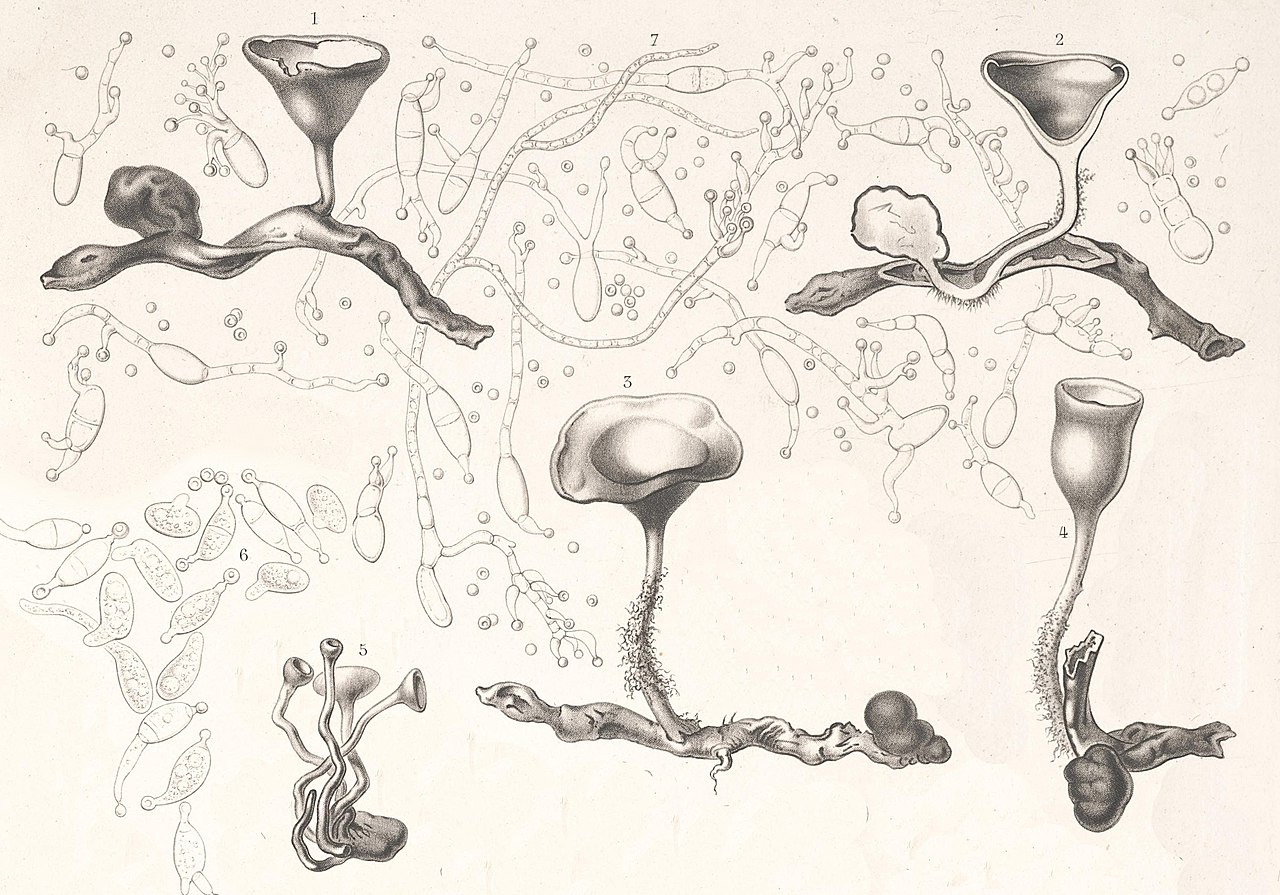
\includegraphics[width=0.9\textwidth]{Figures/PezizaTuberosa.jpg}
        \caption{Caption for figure 1.}
        \label{fig:figure-02.1}
    \end{subfigure}
    \hspace{.5cm} % Adjust the space as needed.
    \begin{subfigure}{0.45\textwidth}
        \centering
        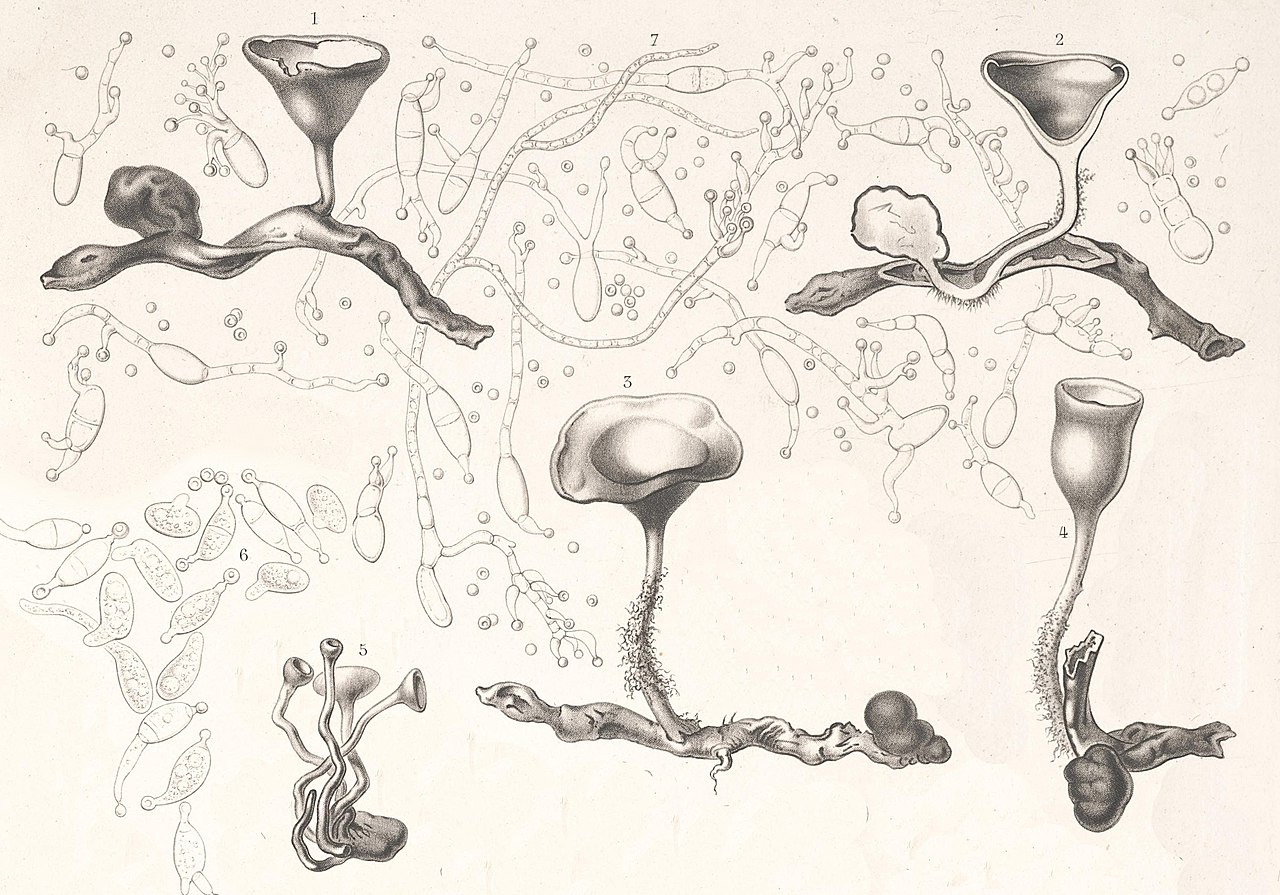
\includegraphics[width=0.9\textwidth]{Figures/PezizaTuberosa.jpg}
        \caption{Caption for figure 2.}
        \label{fig:figure-02.2}
    \end{subfigure}
    \caption{Overall caption of the figure.}
    \label{fig:figure-02}
\end{figure}

\section{Tables}
Tables are vital for presenting findings effectively. This chapter explores techniques for conveying information through tables using various template environments. Defining tables in \LaTeX\ seems complex, but this template simplifies the process.

\begin{block}[tip]
\textit{Prior to showcasing the different table environments, it's crucial to note that each one must be enclosed within a \texttt{\textbackslash begin\{table\}} environment. Additionally, it is recommended to utilise the \texttt{[!htpb]} float options for improved document placement. \textbf{This advice should be taken into consideration when positioning figures as well}.}
\end{block}

\subsection{Tabular Environment}
The conventional \verb|\begin{tabular}| environment enables you to create a simple yet elegant table. \autoref{tab:table-01} is generated using a centering environment for added emphasis. It also incorporates the \verb|booktab| configuration for a more sophisticated table style.

\begin{table}[!htpb]
    \caption{A table showcasing the usage of the tabular environment.}
    \label{tab:table-01}
    \centering
    \begin{tabular}{llc}
        \toprule
        \textbf{Header 01} & \textbf{Header 02} & \textbf{Header 03} \\ 
        \midrule
        Lorem Ipsum         & Pharetra Dolor    & $\checkmark$  \\
        Amet Consectetuer   & Curabitur Aliquet & -             \\
        Praesent Mauris     & Praesent Libero   & $\checkmark$  \\
        \bottomrule
    \end{tabular}
\end{table}

\subsection{Tabularx Environment}
Employ the \verb|\begin{tabularx}| package to construct a table featuring automatically expanding multi-columns. To achieve this automatic behaviour for multi-columns, you can use the following environment: \verb|\begin{tabularx}{\textwidth}{lX}|, where \verb|X| is the column that will function as a multi-column. \autoref{tab:table-02} showcases the usage of the \verb|begin{tabularx}| environment.
%Take note that we substitute \verb|X| in place of \verb|l| or \verb|c|, explicitly indicating that the column will function as a multi-column, occupying the entire available space.

\begin{table}[!htpb]
    \caption{A table showcasing the usage of the tabularx environment.}
    \label{tab:table-02}
    \begin{tabularx}{\textwidth}{lX}
        \toprule
        \textbf{Header 01} & \textbf{Header 02} \\ 
        \midrule
        Foo Bar Baz & Quisque cursus, metus vitae pharetra auctor, sem massa mattis sem, at interdum magna augue eget diam. \\
        Ipsum Dolor & Vestibulum ante ipsum primis in faucibus orci luctus et ultrices posuere cubilia Curae; Curabitur aliquet quam id dui. \\
        Dolor Sit & Phasellus condimentum elementum justo, quis interdum est sagittis ac. Vestibulum non arcu sit amet justo lobortis semper. \\
        Amet Consectetuer & Integer nec odio praesent libero sed cursus ante dapibus diam sed nisi vestibulum non arcu. \\
        Consectetuer Adipiscing & Nulla quis sem at nibh elementum imperdiet. Duis sagittis ipsum. Praesent mauris. \\
        \bottomrule
    \end{tabularx}
\end{table}

\subsection{Longtable Environment}
At times, when dealing with exceptionally lengthy tables, it becomes necessary to split them across multiple pages. In \LaTeX, this can be achieved using the \verb|\begin{longtable}| environment. This environment is slightly more complex than others, as you need to define the header twice: once for the initial appearance of the table and again for when the table spans additional pages. This repeated header ensures the reader can correctly identify the columns on subsequent pages. Feel free to consult \autoref{tab:table-03} for a detailed demonstration of how the \verb|longtable| environment works.

\begin{longtable}[c]{llll}
\caption{A table showcasing the usage of the longtable environment.}
\label{tab:table-03} \\
\toprule
\textbf{Names} & \textbf{E-Mails} & \textbf{Job/Role} \\ \midrule
\endfirsthead
%
\multicolumn{4}{c}%
{{\textit{\bfseries Table \thetable\ continued from previous page.}}} \\
\toprule
\textbf{Names} & \textbf{E-Mails} & \textbf{Job/Role} \\ \midrule
\endhead
%
\bottomrule
\addlinespace[1mm]
\multicolumn{4}{r}%
{{\textit{Continued on the next page.}}} \\
\endfoot
\bottomrule
%
\endlastfoot
%
Alice Johnson & alice.johnson@email.com & Project Manager \\
Bob Thompson & bob.thompson@email.com & Data Analyst \\
Charlie Davis & charlie.davis@email.com & Marketing Specialist \\
David Miller & david.miller@email.com & QA Tester \\
Emily White & emily.white@email.com & Graphic Designer \\
Frank Martin & frank.martin@email.com & HR Coordinator \\
Grace Turner & grace.turner@email.com & Financial Analyst \\
Henry Lee & henry.lee@email.com & System Administrator \\
Ivy Carter & ivy.carter@email.com & Customer Support \\
Jack Wilson & jack.wilson@email.com & Frontend Developer \\
Jane Reed & jane.reed@email.com & UX Designer \\
Kevin Evans & kevin.evans@email.com & Product Manager \\
Linda Adams & linda.adams@email.com & Accountant \\
Mike Hill & mike.hill@email.com & Network Engineer \\
Nina Garcia & nina.garcia@email.com & Business Analyst \\
Oliver Smith & oliver.smith@email.com & Sales Representative \\
Pamela Turner & pamela.turner@email.com & Legal Counsel \\
Quincy Brown & quincy.brown@email.com & IT Consultant \\
Rachel Moore & rachel.moore@email.com & Content Writer \\
Samuel White & samuel.white@email.com & Research Scientist \\ 
Amy Harris & amy.harris@email.com & Digital Strategist \\
Brian Cook & brian.cook@email.com & Operations Manager \\
Catherine Ross & catherine.ross@email.com & Brand Manager \\
Daniel Green & daniel.green@email.com & Database Administrator \\
Emma Taylor & emma.taylor@email.com & Social Media Manager \\
Felix Carter & felix.carter@email.com & Compliance Officer \\
Gloria Scott & gloria.scott@email.com & Procurement Specialist \\
Harold Bennett & harold.bennett@email.com & DevOps Engineer \\
Isla Cooper & isla.cooper@email.com & User Researcher \\
James Black & james.black@email.com & Mobile App Developer \\
Katie Brown & katie.brown@email.com & UI Designer \\
Leo Perez & leo.perez@email.com & Scrum Master \\
Megan Clark & megan.clark@email.com & Event Coordinator \\
Nathan Ward & nathan.ward@email.com & Security Analyst \\
Olivia Harris & olivia.harris@email.com & Corporate Trainer \\
Paul King & paul.king@email.com & Territory Manager \\
Queen Foster & queen.foster@email.com & Paralegal \\
Rebecca Adams & rebecca.adams@email.com & Copy Editor \\
Steven Martin & steven.martin@email.com & Robotics Engineer \\
\end{longtable}

\subsection{Complex Tables}
Creating intricate tables in \LaTeX\ can be a somewhat challenging task. Therefore, we highly recommend using the \href{https://www.tablesgenerator.com/}{Table Generator}. With this tool, you can design your table with the desired style and then easily copy and paste it into your document. This approach simplifies the process and helps ensure the accurate representation of complex tables in your \LaTeX\ document. However, it's crucial to keep in mind that a table should be easily comprehensible for the reader and should not be overly complex. \textbf{The complexity of a table may impede understanding.} For example, \autoref{tab:table-04} presents a table with intricate details.

\begin{table}[!htpb]
    \caption{A table showcasing the usage of the complex tables.}
    \label{tab:table-04}
    \centering
    \begin{tabular}{lcc}
        \toprule
        \multirow{2}{*}{\textbf{Component}} & \multicolumn{2}{c}{\textbf{Specifications}} \\
        \cmidrule(lr){2-3}
        & \textbf{Characteristic} & \textbf{Supported} \\
        \midrule
        \multirow{4}{*}{CPU} & Core Count (e.g., 8 Cores) & $\checkmark$ \\
        & Clock Speed (e.g., 3.6 GHz) & $\checkmark$ \\
        & Hyper-Threading & $\checkmark$ \\
        & Integrated Graphics & - \\
        \midrule
        \multirow{4}{*}{GPU} & CUDA Cores (e.g., 5120) & $\checkmark$ \\
        & Base Clock (e.g., 1.5 GHz) & $\checkmark$ \\
        & Ray Tracing Support & $\checkmark$ \\
        & Multi-GPU Support (SLI/CrossFire) & - \\
        \midrule
        \multirow{4}{*}{Memory} & Type (e.g., DDR5, GDDR6) & $\checkmark$ \\
        & Capacity (e.g., 16 GB) & $\checkmark$ \\
        & Memory Bandwidth (e.g., 448 GB/s) & $\checkmark$ \\
        & ECC Support & - \\
        \midrule
        \multirow{3}{*}{Motherboard Features} & PCIe 5.0 Support & $\checkmark$ \\
        & Wi-Fi 6E & $\checkmark$ \\
        & Thunderbolt 4 & - \\
        \bottomrule
    \end{tabular}
\end{table}

\section{Lists}
Creating lists in \LaTeX\ is straightforward, offering various options to suit your needs. You can generate a bullet list using \verb|\begin{itemize}|, or opt for a numbered list with \verb|\begin{enumerate}|. Below is an example with the \verb|\begin{itemize}| environment.

\begin{itemize}
  \item List entries start with the \verb|\item| command.
  \item Individual entries are indicated with a black dot, a so-called bullet.
  \item The text in the entries may be of any length.
\end{itemize}

As mentioned earlier, you can generate a numbered list using the \verb|\begin{enumerate}| environment. Here is an example:

\begin{enumerate}
  \item Items are numbered automatically.
  \item The numbers start at 1 with each use of the \verb|enumerate| environment.
  \item Another entry in the list.
\end{enumerate}

You can also nest list entries by creating a list inside another list of the same type. Here is an example:

\begin{enumerate}
    \item First level item
    \item First level item
    \begin{enumerate}
        \item Second level item
        \item Second level item
    \begin{enumerate}
        \item Third level item
        \item Third level item
    \end{enumerate}
    \end{enumerate}
\end{enumerate}

\begin{block}[tip]
\textit{Please note that the labels change automatically regardless of the environment being the same for every list. \textbf{This demonstrates that there's no need to worry about changing the environment for something different.}}
\end{block}

You can also modify the label of your list to something entirely different that suits your needs. To accomplish this, insert a new \verb|\item| and enclose your desired label in square brackets. For example, \verb|\item[!]| will result in an exclamation point as your new label. Below are some examples of modified labels.

\begin{itemize}
  \item This is my first point
  \item Another point I want to make 
  \item[!] A point to exclaim something!
  \item[$\blacksquare$] Make the point fair and square.
  \item[] A blank label?
\end{itemize}

Finally, you can create a description list. Unlike having a bullet point or a numbered label, a description list enables you to use custom descriptions that suit your list. In the example below, there are three \verb|\item| entries: one without a label, and two with descriptions.

\begin{description}
    \item[Item 1:] This is the first item with a description.
    \item[Item 2:] Another item with a different description.
    \item An item without a specific label.
\end{description}

\section{Code Listings}
At times, you may want to include source code from your programs and applications within your document. To achieve this, you can use two nested environments: \verb|\begin{listing}| to create a listing with both caption and label, and \verb|\begin{minted}| for code highlighting. \autoref{listing:c-code} provides an example of a source code in C.

\begin{listing}[!htpb]
\caption{Hello world in C.}
\label{listing:c-code}
\begin{minted}{c}
#include <stdio.h>
int main() {
  printf("Hello, World!"); /* printf() outputs the quoted string */
  return 0;
}
\end{minted}
\end{listing}

The code mentioned above was inserted into the document. However, an alternative approach is to input your code from an external file. To do so, you just need to use the command \verb|\inputminted{CODE_LANGUAGE}{FILE}|. Of course, you should place that command inside of the \verb|\begin{listing}| environment. \autoref{listing:haskell-code} illustrates an example of Haskell source code that has been input from an external file.

\begin{listing}[!htpb]
\caption{Factorial in Haskell.}
\label{listing:haskell-code}
\inputminted{haskell}{Code/Factorial.hs}
\end{listing}

In some cases, when you simply want to highlight a specific command, it's recommended not to use \verb|listing| or \verb|minted|. Instead, you should utilise the \verb|\verb| command for inline highlighting or the \verb|\begin{verbatim}| environment for longer sections of highlighted code. An example of a lengthy \verb|verbatim| section is provided below, demonstrating how to create a \verb|listing| with an input code:

\begin{verbatim}
\begin{listing}[!htpb]
    \inputminted{CODE_LANGUAGE}{FILE}
    \caption{TEXT}
    \label{TEXT}
\end{listing}
\end{verbatim}

Sometimes it is necessary to display longer code that occupies more than one page. For this purpose, please use the environment \verb|\begin{longlisting}|. This environment will easily break your code into multiple pages for better readability without you worrying about the size of your code. An example is shown below in \autoref{listing:lisp-code}.

\begin{longlisting}
\caption{A sample of functions in Lisp.}
\label{listing:lisp-code}
\begin{minted}{lisp}
(defun factorial (n)
 "Calculate the factorial of a number."
 (if (zerop n)
     (* n (factorial (1- n)))))

(defun fibonacci (n)
 "Calculate the nth Fibonacci number."
 (cond ((zerop n) 0)
       ((= n 1) 1)
       (t (+ (fibonacci (1- n)) (fibonacci (- n 2))))))

(defun gcd (a b)
 "Calculate the greatest common divisor of a and b."
 (if (zerop b)
     a
     (gcd b (mod a b))))

(defun primes-up-to (limit)
 "Return a list of all prime numbers up to LIMIT."
 (let ((primes '()))
   (loop for i from 2 to limit
         unless (some (lambda (p) (zerop (mod i p))) primes)
         do (push i primes))
   (nreverse primes)))

(defun example-function (x)
 "An example function to demonstrate Lisp capabilities."
 (let ((result (list (factorial x)
                     (fibonacci x)
                     (gcd x 10)
                     (primes-up-to x))))
   (format t "Factorial of ~A: ~A~%" x (factorial x))
   (format t "Fibonacci of ~A: ~A~%" x (fibonacci x))
   (format t "GCD of ~A and 10: ~A~%" x (gcd x 10))
   (format t "Primes up to ~A: ~A~%" x (primes-up-to x))
   result))

(example-function 10)
\end{minted}
\end{longlisting}

\section{Equations}
When writing equations and other mathematical expressions, \LaTeX~is a powerful and versatile tool. You can enter a formula in inline mode using the environment \verb|\(FORMULA\)| or use \verb|\begin{equation}| to display it in ``math mode'' with numbering. If you prefer not to display the equation number, you can use the environment \verb|\[FORMULA\]|.

\vspace{.875em}
\textbf{Example:} In physics, the mass-energy equivalence is expressed by the equation \(E=mc^2\), discovered in 1905 by Albert Einstein. In natural units ($c = 1$), the formula (\ref{eq:equation-01}) expresses the identity:

\begin{equation}
\label{eq:equation-01}
E=m
\end{equation}

\textbf{Example:} Below is a equation -- \textit{without numbering} -- for the regularised loss function in supervised learning, combining the average prediction loss over the training dataset and an $L_2$ regularisation term to prevent overfitting:

\[
\mathcal{L}(\boldsymbol{\theta}) = \frac{1}{N} \sum_{i=1}^{N} \ell(y_i, f(\mathbf{x}_i; \boldsymbol{\theta})) + \lambda \|\boldsymbol{\theta}\|_2^2
\]

Equations can be a bit challenging to create, so we advise using an online editor, like the \href{https://latexeditor.lagrida.com/}{LaTeX Equation Editor}. Simply build your formulas there and copy and paste them into your document, either inline or in a math block, as shown above.

\section{Footnotes}
Sometimes it is important to present information that is not central to the main text in a footnote. In \LaTeX\, this can be easily achieved using the command \verb|\footnote{TEXT}|. The text will appear at the bottom of the page\footnote{This is a simple footnote.}.

If you want to use footnotes within tables, it is best to reconsider, as \LaTeX\ does not provide an easy way to handle them. Instead, you can place a ``*'' wherever you want the footnote reference to appear. Then, below the table \textbf{but before ending the table environment}, place the ``*'' along with the footnote text. This will create a similar footnote, but it will appear below the table rather than at the bottom of the page.
}

% \ifthenelse{\equal{\LanguageOption}{portuguese}}{
%     \addtocontents{toc}{\protect\contentsline{chapter}{Apêndices}{}{}}
% }{
%     \addtocontents{toc}{\protect\contentsline{chapter}{Appendices}{}{}}
% }

% \ifthenelse{\equal{\MediaOption}{paper}}{\blankpage}{\clearpage}
% \begin{center}
%     \crimsonfont
%     \thispagestyle{empty}
        
%     \vspace*{\fill}
%     \ifthenelse{\equal{\LanguageOption}{portuguese}}{%
%         {\LARGE\fontsize{26}{26}\selectfont\textcolor{maincolor}{Apêndices}\par}
%     }{%
%         {\LARGE\fontsize{26}{26}\selectfont\textcolor{maincolor}{Appendices}\par}
%     }
%     \vspace*{\fill}
% \end{center}
% \MediaOptionLogicBlank



\ifthenelse{\equal{\LanguageOption}{portuguese}}{%
    % \chapter*{Bibliography}
    \addtocontents{toc}{\protect\contentsline{chapter}{Bibliography}{\thepage}{}}
}{%
    % \chapter*{Bibliography}
    \addtocontents{toc}{\protect\contentsline{chapter}{Bibliography}{\thepage}{}}
}

\printbibliography



\MediaOptionLogicBlank

%%% Appendices: Work that *YOU* Developed %%%
\appendix
\ifthenelse{\equal{\LanguageOption}{portuguese}}{
    \addtocontents{toc}{\protect\contentsline{chapter}{Apêndices}{}{}}
}{
    \addtocontents{toc}{\protect\contentsline{chapter}{Appendices}{}{}}
}

\ifthenelse{\equal{\MediaOption}{paper}}{\blankpage}{\clearpage}
\begin{center}
    \crimsonfont
    \thispagestyle{empty}
        
    \vspace*{\fill}
    \ifthenelse{\equal{\LanguageOption}{portuguese}}{%
        {\LARGE\fontsize{26}{26}\selectfont\textcolor{maincolor}{Apêndices}\par}
    }{%
        {\LARGE\fontsize{26}{26}\selectfont\textcolor{maincolor}{Appendices}\par}
    }
    \vspace*{\fill}
\end{center}
\MediaOptionLogicBlank
\chapter{Benchmark Functions Overview}\label{app:benchmarks_formulas}

This appendix provides an overview of all benchmark functions utilized in this study. For each function, the mathematical formulation is presented, followed by a two-di\-men\-sional plot that visually illustrates the function’s landscape. These materials are intended to facilitate understanding of the test problems and support the interpretation of experimental results discussed in the main text.

% \begin{small}
% \enlargethispage{3\baselineskip}
\paragraph{Alpine N.1}
% \small{non-differentiable, separable, multimodal}
\begin{equation}
f(\mathbf{x})
= \sum_{j=1}^{d} \bigl| x_j \sin(x_j) + 0.1\,x_j \bigr|
\label{ben:alpine}
\end{equation}

\vspace{.095em}
\paragraph*{Crowned Cross}
% \small{non-differentiable, non-separable, multimodal}
\begin{equation}
f(\mathbf{x})
=0.0001\Bigl(\bigl|\exp\!\bigl(\lvert100-\|\mathbf{x}\|/\pi\rvert\bigr)\prod_{j=1}^d\sin(x_j)\bigr|+1\Bigr)^{0.1}
\label{ben:crowned_cross}
\end{equation}

\vspace{.095em}
\paragraph{Egg Holder}
% \small{non-differentiable, non-separable, multimodal}
\begin{equation}
f(\mathbf{x})
= \sum_{j=1}^{d-1}\Bigl[
    -\,x_{j}\,\sin\!\bigl(\sqrt{\lvert x_{j} - (x_{j+1}+47)\rvert}\bigr)
- (x_{j+1}+47)\,\sin\!\bigl(\sqrt{\bigl\lvert \tfrac{x_{j}}{2} + (x_{j+1}+47)\bigr\rvert}\bigr)
\Bigr]
\label{ben:eggHolder}
\end{equation}

\vspace{.095em}
\paragraph{Expanded Shaffer (Schaffer F6)}
% \small{differentiable, non-separable, multimodal}
\begin{equation}
f(\mathbf{x})
= \sum_{j=1}^{d}\Biggl[
    0.5
    + \frac{\sin^2\!\bigl(\sqrt{x_{j}^2 + x_{j+1}^2}\bigr)\;-\;0.5}
           {\bigl(1 + 0.001\,(x_{j}^2 + x_{j+1}^2)\bigr)^{2}}
\Biggr]
\quad
(x_{d+1}\equiv x_{1})
\label{ben:expandedShaffer}
\end{equation}

\vspace{.095em}
\paragraph{Generalized Schaffer N-1}
\begin{equation}
f(\mathbf{x})
= \sum_{j=1}^{d-1}
  \Bigl[
    0.5
    + \frac{\sin^2\!\bigl(x_j^2 - x_{j+1}^2\bigr)\;-\;0.5}
           {\bigl(1 + 0.001\,(x_j^2 + x_{j+1}^2)\bigr)^{2}}
  \Bigr]
\label{ben:generalizedSchafferN1}
\end{equation}

\vspace{.095em}
\paragraph{Generalized Schaffer N-2}
\begin{equation}
f(\mathbf{x})
= -\Bigl(
    \sum_{j=1}^{d-1}
      \Bigl[
        0.5
        + \frac{\cos\!\bigl(\sin\lvert x_j^2 - x_{j+1}^2\rvert\bigr)\;-\;0.5}
               {\bigl(1 + 0.001\,(x_j^2 + x_{j+1}^2)\bigr)^{2}}
      \Bigr]
    - (d-1)
  \Bigr)
\label{ben:generalizedSchafferN2}
\end{equation}

\vspace{.095em}
\paragraph{Generalized Schaffer N-3}
\begin{equation}
f(\mathbf{x})
= \sum_{j=1}^{d-1}
  \bigl(x_j^2 + x_{j+1}^2\bigr)^{\tfrac14}
  \Bigl[
    1
    + \sin^2\!\bigl(50\,(x_j^2 + x_{j+1}^2)^{\tfrac{1}{10}}\bigr)
  \Bigr]
\label{ben:generalizedSchafferN3}
\end{equation}

\vspace{.095em}
\paragraph{Generalized Schaffer N-4}
\begin{equation}
f(\mathbf{x})
= -\Bigl(
    \sum_{j=1}^{d-1}
      \Bigl[
        0.5
        + \frac{\cos\!\bigl(\sin\lvert x_j^2 - x_{j+1}^2\rvert\bigr)\;-\;0.5}
               {\bigl(1 + 0.001\,(x_j^2 + x_{j+1}^2)^2\bigr)^{2}}
      \Bigr]
    - (d-1)
  \Bigr)
\label{ben:generalizedSchafferN4}
\end{equation}

\vspace{.095em}
\paragraph{Generalized Schmidt–Vetters}
\begin{equation}
f(\mathbf{x})
= \sum_{j=1}^{d-1}
  \frac{\sin^2\!\bigl(x_j^2 - x_{j+1}^2\bigr)
        + \cos^2\!\bigl(x_j^2 + x_{j+1}^2\bigr)
        - 1}
       {\bigl(1 + 0.001\,(x_j^2 + x_{j+1}^2)\bigr)^2}
\label{ben:generalizedSchmidtVetters}
\end{equation}

\vspace{.095em}
\paragraph{Lennard–Jones Minimum Energy Cluster}
\begin{equation}
f(\mathbf{x})
= \sum_{1 \,\le\, i < j \,\le\, n}
  \Bigl[\|\mathbf{r}_i - \mathbf{r}_j\|^{-12}
        - 2\,\|\mathbf{r}_i - \mathbf{r}_j\|^{-6}\Bigr],
\quad n = \tfrac{d}{3},\;\mathbf{r}_i=(x_{3i-2},x_{3i-1},x_{3i})
\label{ben:lennardJonesMinimumEnergyCluster}
\end{equation}

\vspace{.095em}
\paragraph{Michalewicz}
\begin{equation}
f(\mathbf{x})
= -\sum_{j=1}^{d}
    \sin(x_j)\,
    \Bigl[\sin\!\Bigl(\tfrac{j\,x_j^2}{\pi}\Bigr)\Bigr]^{2m}
\label{ben:michalewicz}
\end{equation}

\vspace{.095em}
\paragraph{Mishra-03}
\begin{equation}
f(\mathbf{x})
= \sqrt{\left|\cos\!\Bigl(\sqrt{\bigl|\sum_{j=1}^d x_j^2\bigr|}\Bigr)\right|}
  + 0.01 \sum_{j=1}^d x_j
\label{ben:Mishra03}
\end{equation}

\vspace{.095em}
\paragraph{Mishra-04}
\begin{equation}
f(\mathbf{x})
= \sqrt{\left|\sin\!\Bigl(\sqrt{\bigl|\sum_{j=1}^d x_j^2\bigr|}\Bigr)\right|}
  + 0.01 \sum_{j=1}^d x_j
\label{ben:Mishra04}
\end{equation}

\vspace{.095em}
\paragraph{Modified Rosenbrock N.2}
\begin{equation}
f(\mathbf{x})
= \sum_{j=1}^{d-1}\bigl[\,100\,\sqrt{\lvert x_{j+1} - x_j^2\rvert}\;+\;(1 - x_j)^2\bigr]
\label{ben:RosenbrockModified02}
\end{equation}

\vspace{.095em}
\paragraph{Rotated Bent Cigar}
\begin{equation}
f(\mathbf{x})
= z_1^2 \;+\; 10^6 \sum_{j=2}^d z_j^2,
\quad \mathbf{z} = \mathbf{M}\,\mathbf{x}
\label{ben:RotatedBentCigar}
\end{equation}

\vspace{.095em}
\paragraph{Rotated Discus}
\begin{equation}
f(\mathbf{x})
= 10^6\,z_1^2 \;+\; \sum_{j=2}^d z_j^2,
\quad \mathbf{z} = \mathbf{M}\,\mathbf{x}
\label{ben:RotatedDiscus}
\end{equation}

\enlargethispage{\baselineskip}
\vspace{.095em}
\paragraph{Rotated High Conditioned Elliptic}
\begin{equation}
f(\mathbf{x})
= \sum_{j=1}^d 10^{6\,\frac{j-1}{d-1}}\,z_j^2,
\quad \mathbf{z} = \mathbf{M}\,\mathbf{x}
\label{ben:RotatedHighConditionedElliptic}
\end{equation}

\vspace{.095em}
\paragraph{Salomon}
\begin{equation}
f(\mathbf{x})
= 1 \;-\;\cos\!\Bigl(2\pi\sqrt{\sum_{j=1}^d x_j^2}\Bigr)
\;+\;0.1\,\sqrt{\sum_{j=1}^d x_j^2}
\label{ben:Salomon}
\end{equation}

\vspace{.095em}
\paragraph{Schwefel N.2.0}
\begin{equation}
f(\mathbf{x})
= \max_{1\le i\le d}\Bigl|\sum_{j=1}^{i} x_j\Bigr|
\label{ben:SchwefelN20}
\end{equation}

\vspace{.095em}
\paragraph{Schwefel N.3.6}
\begin{equation}
f(\mathbf{x})
= \sum_{j=1}^{d-1}\Bigl[-\,x_j\,x_{j+1}\,(72 - 2x_j - 2x_{j+1}) + 3456\Bigr] \\
 + (d-1)\times 4.8\times10^8
\label{ben:SchwefelN36}
\end{equation}

\vspace{.095em}
\paragraph{Schwefel N.6}
\begin{equation}
f(\mathbf{x})
= \Bigl|\sum_{j=1}^{d} x_j\Bigr| \;+\; \sum_{j=1}^{d} |x_j|
\label{ben:SchwefelN6}
\end{equation}

\vspace{.095em}
\paragraph{Shifted Schwefel (N.2.6)}
\begin{equation}
f(\mathbf{x})
= 418.9829\,d \;-\;\sum_{j=1}^{d} z_j\,\sin\!\bigl(\sqrt{|z_j|}\bigr),
\quad \mathbf{z} = \mathbf{x} - \mathbf{s}
\label{ben:ShiftedSchwefel}
\end{equation}

\vspace{.095em}
\paragraph{Shifted and Rotated HappyCat}
\begin{equation}
f(\mathbf{x})
= \left\lvert\sum_{j=1}^d z_j^2 - d\right\rvert^{\tfrac14}
+ \frac{0.5\sum_{j=1}^d z_j^2 + \sum_{j=1}^d z_j}{d}
+ 0.5,
\quad \mathbf{z} = \mathbf{M}\,\bigl(\mathbf{x}-\mathbf{s}\bigr)
\label{ben:ShiftedRotatedHappyCat}
\end{equation}

\vspace{.095em}
\paragraph{Shifted and Rotated HGBat}
\begin{equation}
f(\mathbf{x})
= \sqrt{\bigl\lvert(\sum_{j=1}^d z_j^2)^2 - (\sum_{j=1}^d z_j)^2\bigr\rvert}
+ \frac{0.5\sum_{j=1}^d z_j^2 + \sum_{j=1}^d z_j}{d}
+ 0.5,
\quad \mathbf{z} = \mathbf{M}\,\bigl(\mathbf{x}-\mathbf{s}\bigr)
\label{ben:ShiftedRotatedHGBat}
\end{equation}

\vspace{.095em}
\paragraph{Shifted and Rotated Schaffer F7}
\begin{equation}
f(\mathbf{x})
= \left[\frac{1}{d-1}\sum_{j=1}^{d-1}\Bigl(s_j + s_j\sin^2\!\bigl(50\,s_j^{1/5}\bigr)\Bigr)\right]^2,
\quad \mathbf{z} = 10\,\mathbf{M}\,\bigl(\mathbf{x}-\mathbf{s}\bigr),
\quad s_j = z_j^2 + z_{j+1}^2
\label{ben:ShiftedRotatedSchafferF7}
\end{equation}

% \paragraph{Shifted and Rotated Weierstrass}
% \begin{equation}
% f(\mathbf{x})
% = \sum_{i=1}^d \sum_{k=0}^{20} a^k
% \cos\!\bigl(2\pi\,b^k\,(z_i+0.5)\bigr)
% \;-\;d\,\sum_{k=0}^{20} a^k
% \cos\!\bigl(2\pi\,b^k\,0.5\bigr),
% \quad a=0.5,\;b=3,
% \quad \mathbf{z} = \mathbf{M}\,\bigl(\mathbf{x}-\mathbf{s}\bigr)
% \label{ben:ShiftedRotatedWeierstrass}
% \end{equation}

\vspace{.095em}
\paragraph{Shifted and Rotated Weierstrass}
\begin{equation}
f(\mathbf{x})
= \sum_{i=1}^d \sum_{k=0}^{20} 0.5^k
\cos\!\bigl(2\pi\,(3^k)\,(z_i+0.5)\bigr)
\;-\;d \sum_{k=0}^{20} 0.5^k
\cos\!\bigl(2\pi\,(3^k)\,0.5\bigr),
\quad \mathbf{z} = \mathbf{M}(\mathbf{x}-\mathbf{s})
\label{ben:ShiftedRotatedWeierstrass}
\end{equation}



% \paragraph{Shubert N.3}
% \begin{equation}
% f(\mathbf{x})
% = \sum_{k=1}^{d} S_{3}(x_k),
% \quad
% S_{3}(x) = \sum_{j=1}^{5} \bigl[j\,\sin\bigl((j+1)x\bigr) + j\bigr]
% \label{ben:ShubertN3}
% \end{equation}

% \paragraph{Shubert N.4}
% \begin{equation}
% f(\mathbf{x})
% = \sum_{k=1}^{d} S_{4}(x_k),
% \quad
% S_{4}(x) = \sum_{j=1}^{5} \bigl[j\,\cos\bigl((j+1)x\bigr) + j\bigr]
% \label{ben:ShubertN4}
% \end{equation}

\vspace{.095em}
\paragraph{Shubert N.3}
\begin{equation}
f(\mathbf{x})
= \sum_{k=1}^{d}\sum_{j=1}^{5}\bigl[j\,\sin\bigl((j+1)x_{k}\bigr)+j\bigr]
\label{ben:ShubertN3}
\end{equation}

\vspace{.095em}
\paragraph{Shubert N.4}
\begin{equation}
f(\mathbf{x})
= \sum_{k=1}^{d}\sum_{j=1}^{5}\bigl[j\,\cos\bigl((j+1)x_{k}\bigr)+j\bigr]
\label{ben:ShubertN4}
\end{equation}


\vspace{.095em}
\paragraph{Sine Envelope}
\begin{equation}
f(\mathbf{x})
= -\sum_{j=1}^{d-1}\Bigl[
    \frac{\sin^2\!\bigl(\sqrt{x_j^2 + x_{j+1}^2} - 0.5\bigr)}
         {\bigl(0.001\,(x_j^2 + x_{j+1}^2) + 1\bigr)^2}
    + 0.5
  \Bigr]
\label{ben:SineEnvelope}
\end{equation}

\vspace{.095em}
\paragraph{Stochastic}
\begin{equation}
f(\mathbf{x})
= \sum_{j=1}^{d} \epsilon_j \,\bigl\lvert x_j - \tfrac{1}{j}\bigr\rvert,
\quad \epsilon_j \sim U(0,1)
\label{ben:Stochastic}
\end{equation}

\vspace{.095em}
\paragraph{Stretched V}
\begin{equation}
f(\mathbf{x})
= \sum_{j=1}^{d-1}
  \bigl(x_j^2 + x_{j+1}^2\bigr)^{\tfrac14}
  \Bigl[\sin\!\bigl(50\,\bigl(x_j^2 + x_{j+1}^2\bigr)^{\tfrac1{10}}\bigr) + 1\Bigr]^2
\label{ben:StretchedV}
\end{equation}


\vspace{.095em}
\paragraph{Styblinski–Tang}
\begin{equation}
f(\mathbf{x})
= \tfrac12 \sum_{j=1}^{d}\bigl(x_j^4 - 16\,x_j^2 + 5\,x_j\bigr)
\label{ben:StyblinskiTang}
\end{equation}


% \end{small}
















% \begin{figure}[!htpb]
%     \centering
%     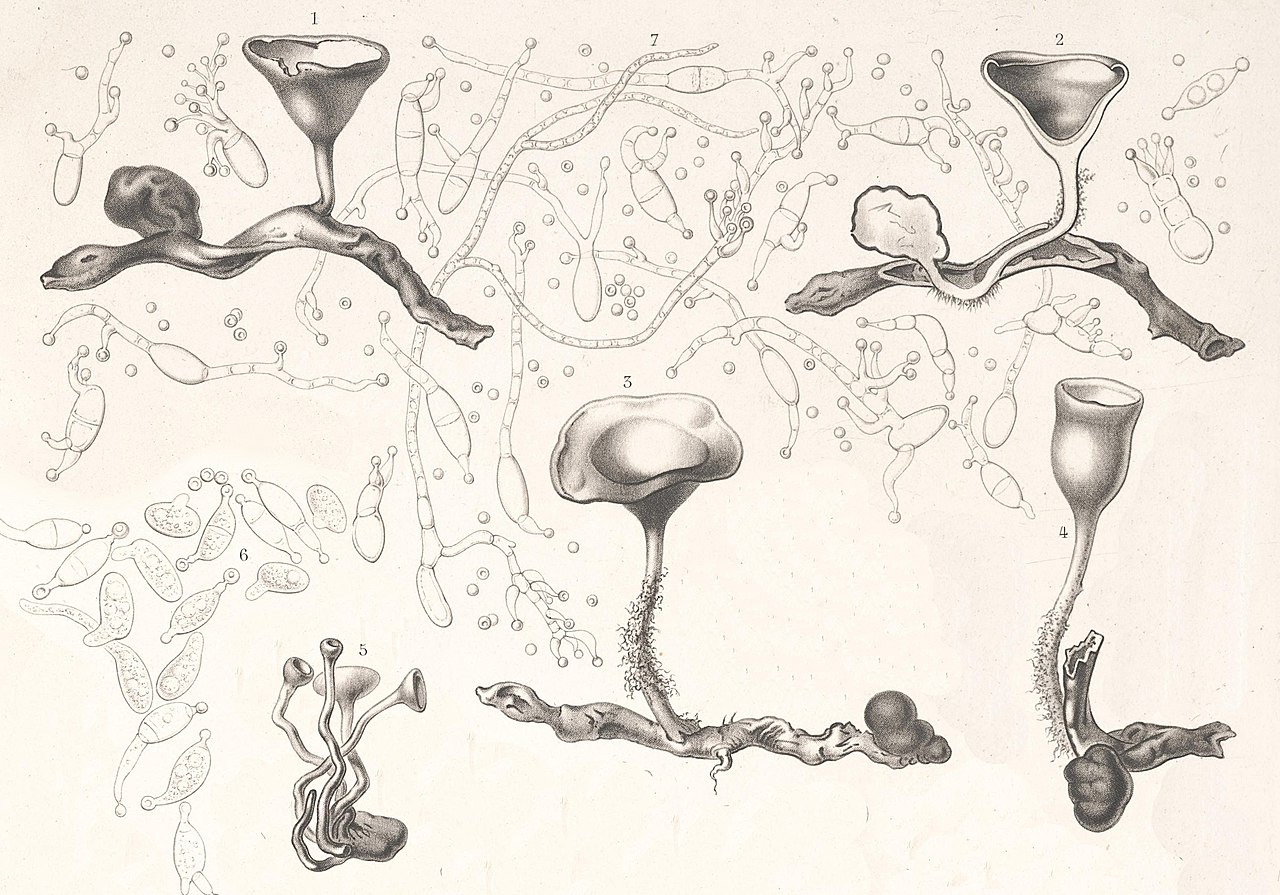
\includegraphics[width=\linewidth]{Figures/PezizaTuberosa.jpg}
%     \caption[Illustration of the fungus Dumontinia tuberosa.]{Illustration of the fungus Dumontinia tuberosa by physician, mycologist, and illustrator Charles Tulasne (1816–1884) in the book Selecta Fungorum Carpologia (1861–65). (Name of the original work: Peziza tuberosa parasite on Anemone nemorosa).}
%     \label{fig:figure-01}
% \end{figure}


\enlargethispage{3\baselineskip}
\begin{figure}[!hb]
\renewcommand\thesubfigure{A.\arabic{subfigure}} % Local change starts here
    \centering
    \begin{subfigure}{0.32\textwidth}
        \centering
        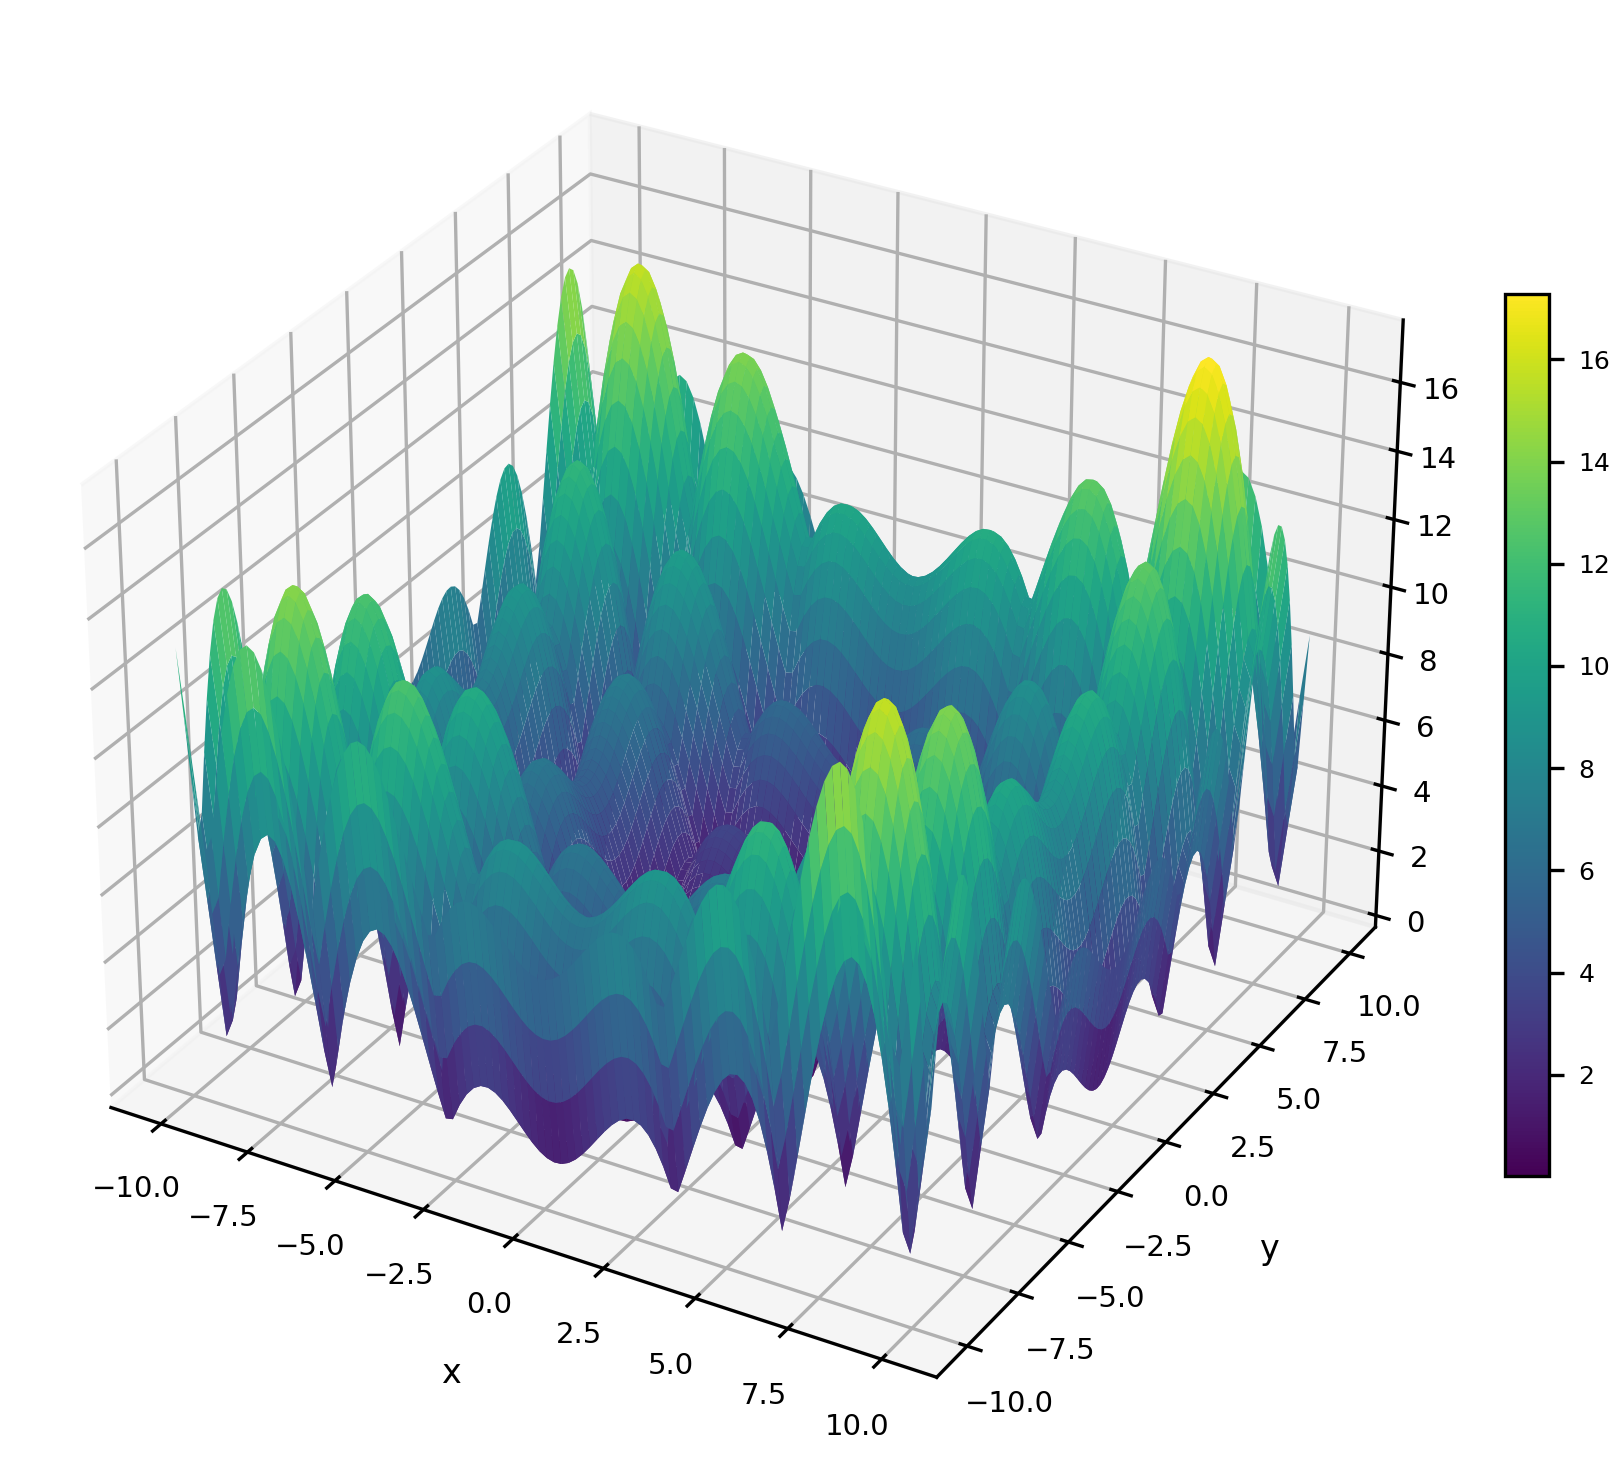
\includegraphics[width=1\textwidth]{Figures/benchmark_plots/Alpine_N1_maximized.png}
        \caption{Alpine N.1}
    \end{subfigure}
    % \hspace{.5cm} % Adjust the space as needed.
    \begin{subfigure}{0.32\textwidth}
        \centering
        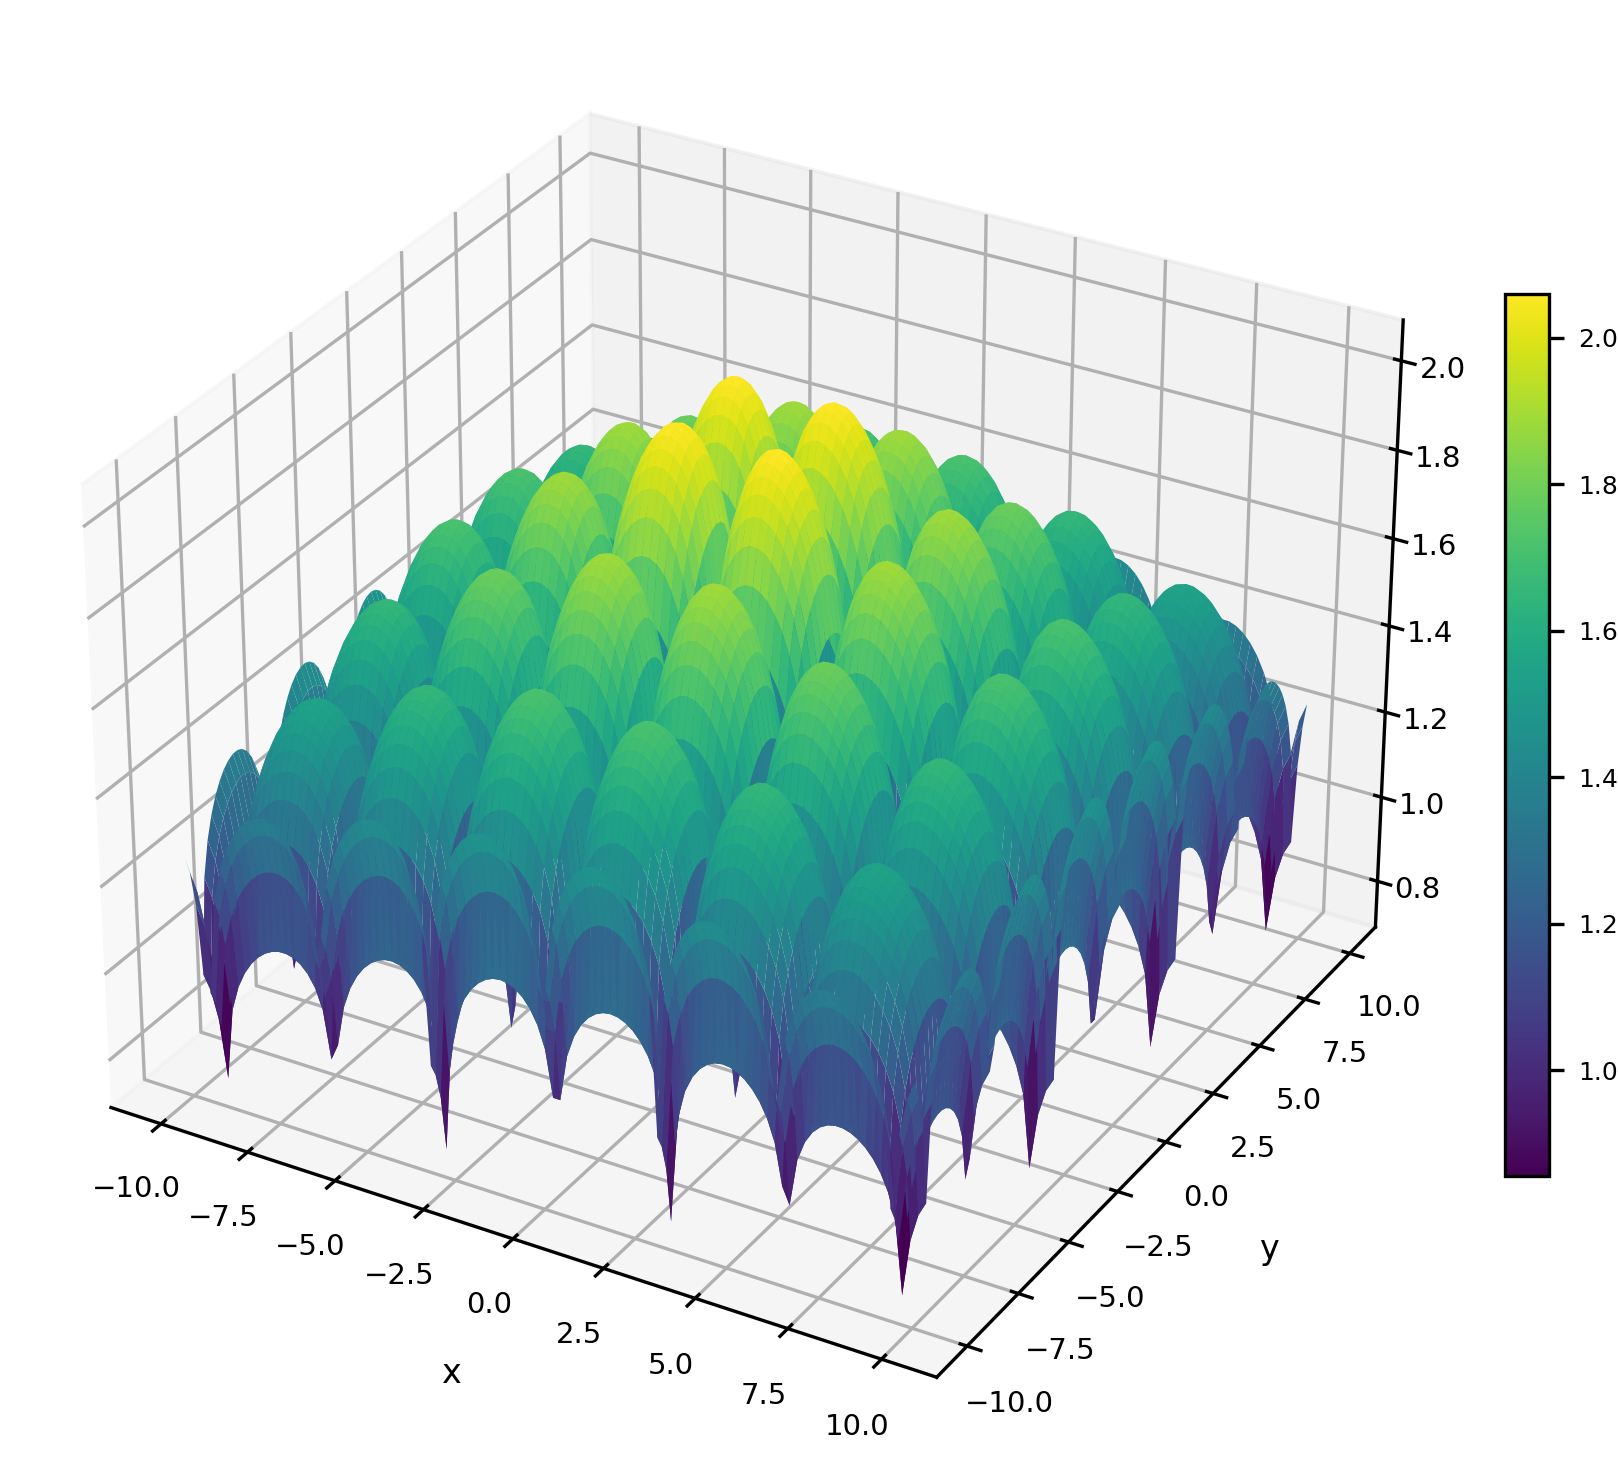
\includegraphics[width=1\textwidth]{Figures/benchmark_plots/Crowned_Cross_maximized.png}
        \caption{Crowned Cross}
    \end{subfigure}
    \begin{subfigure}{0.32\textwidth}
        \centering
        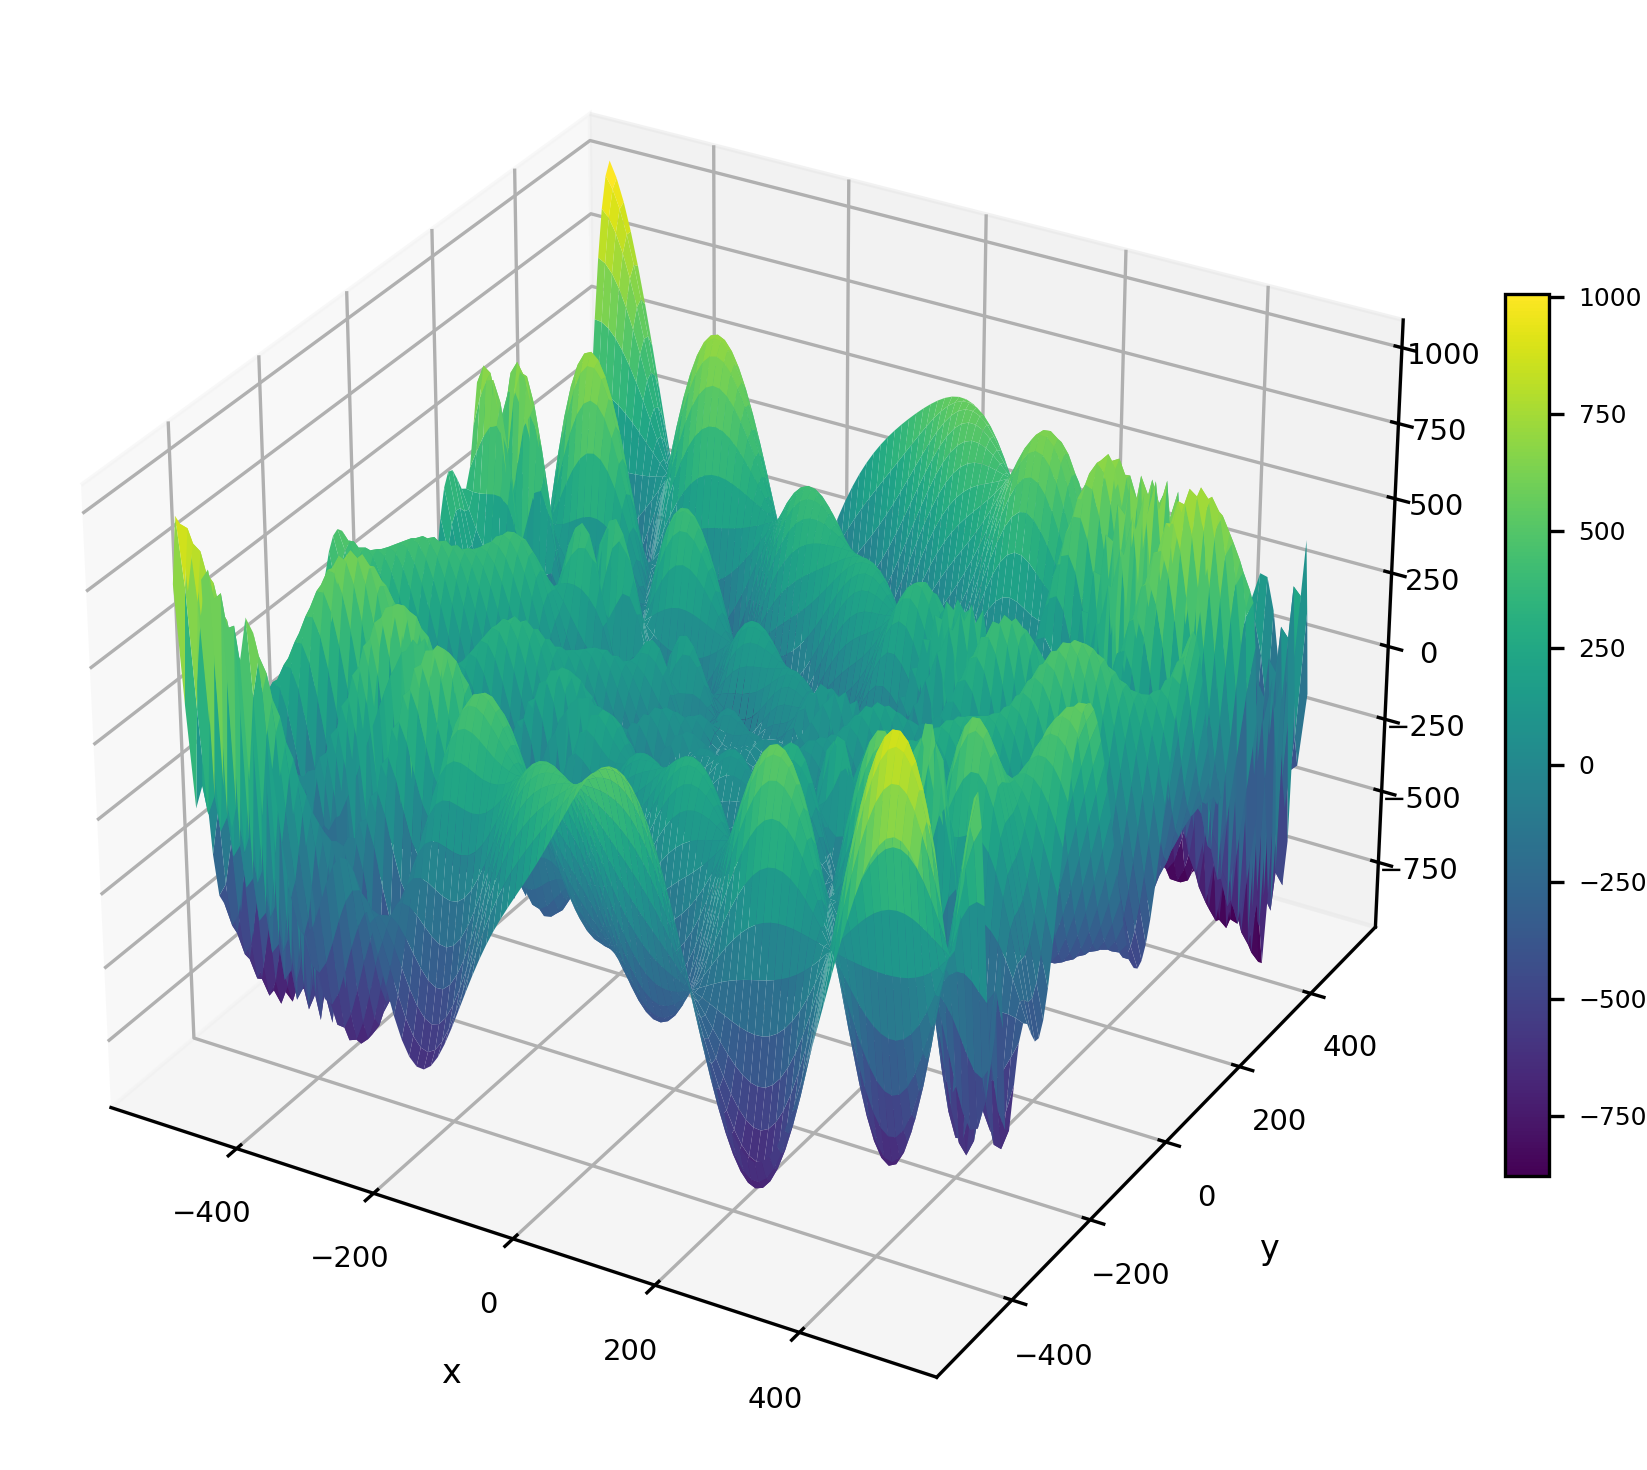
\includegraphics[width=1\textwidth]{Figures/benchmark_plots/Egg_Holder_maximized.png}
        \caption{Egg Holder}
    \end{subfigure}
    % \hspace{.5cm} % Adjust the space as needed.
    \begin{subfigure}{0.32\textwidth}
        \centering
        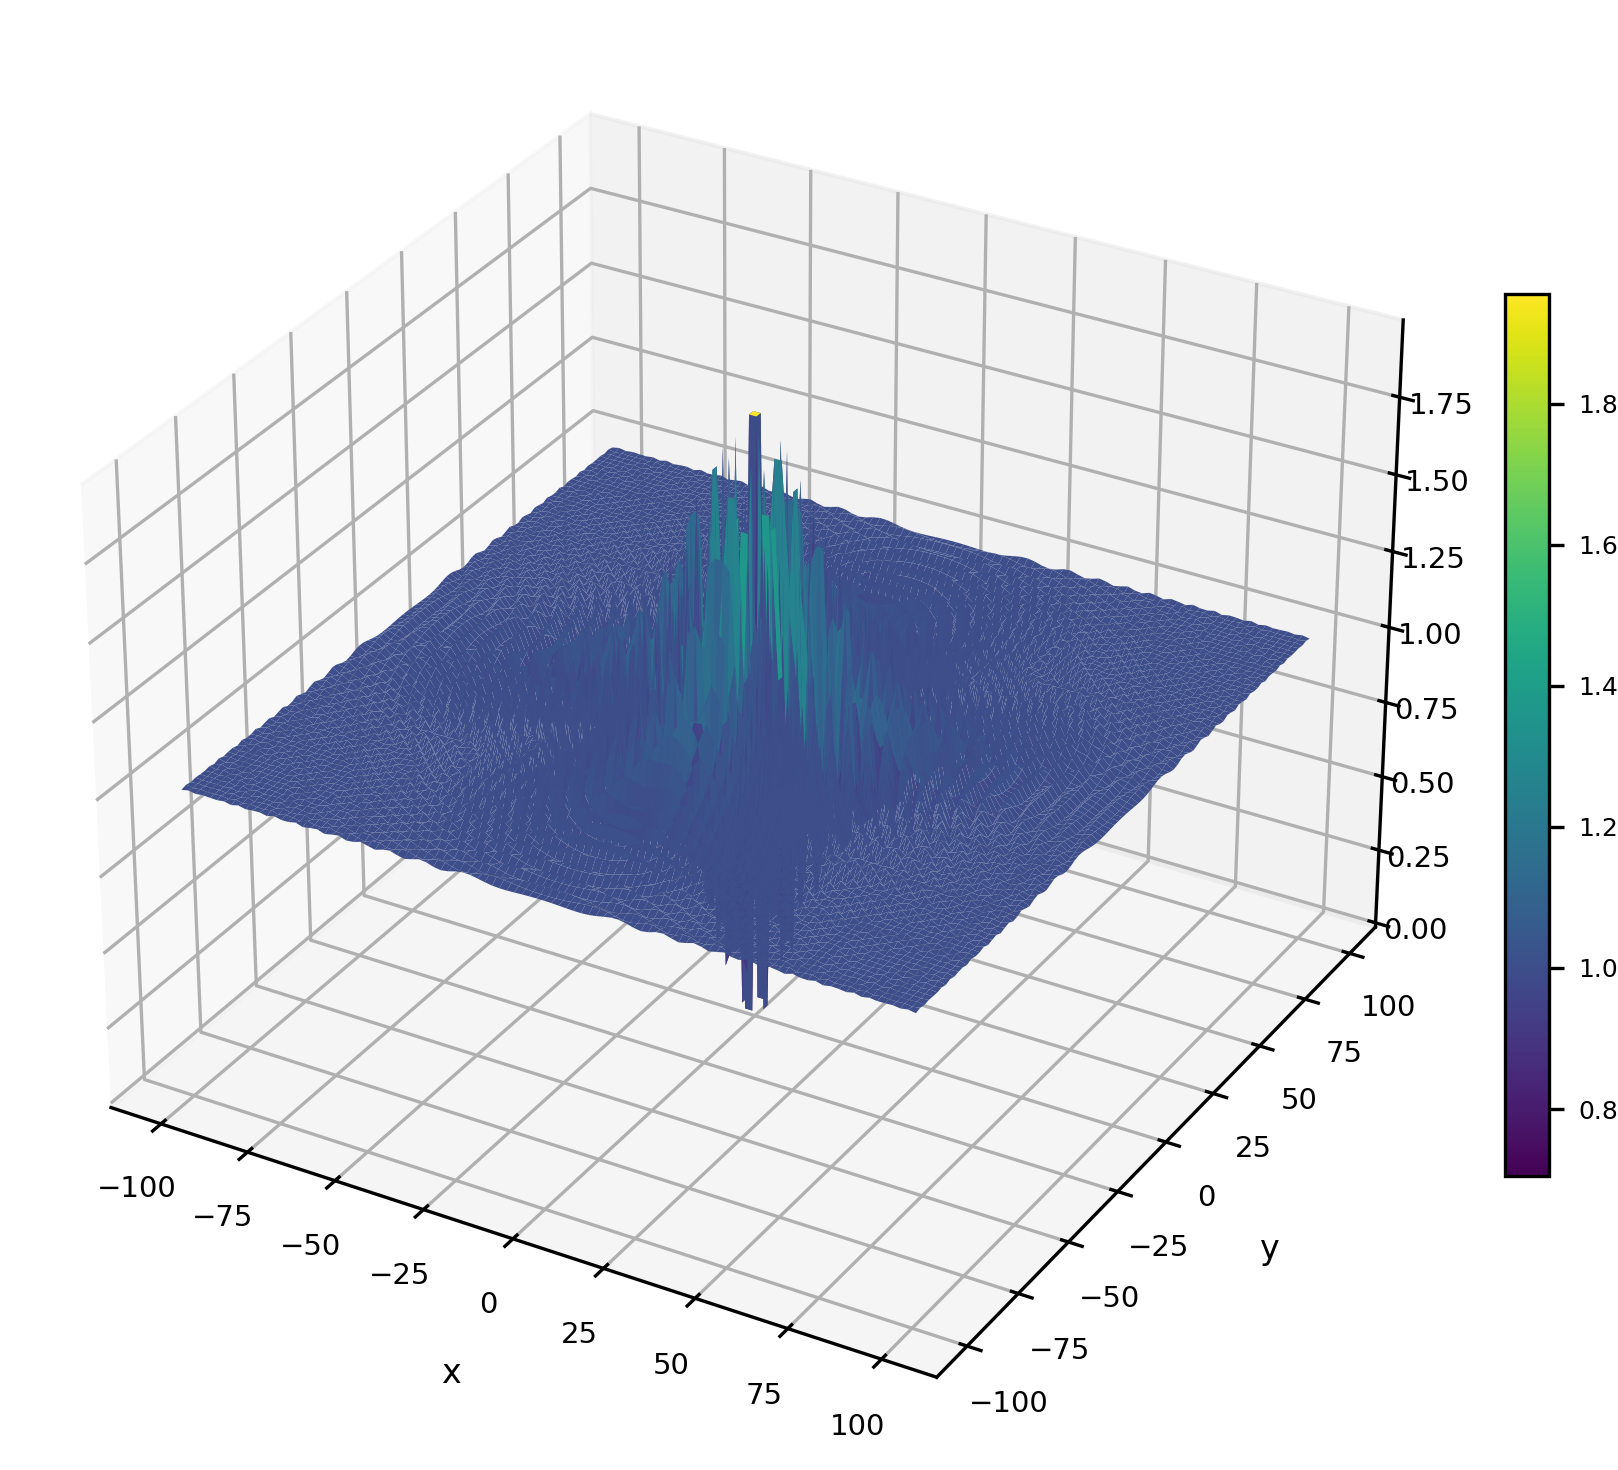
\includegraphics[width=1\textwidth]{Figures/benchmark_plots/Expanded_Shaffer_maximized.png}
        \caption{Expanded Shaffer (F6)}
    \end{subfigure}
        \begin{subfigure}{0.32\textwidth}
        \centering
        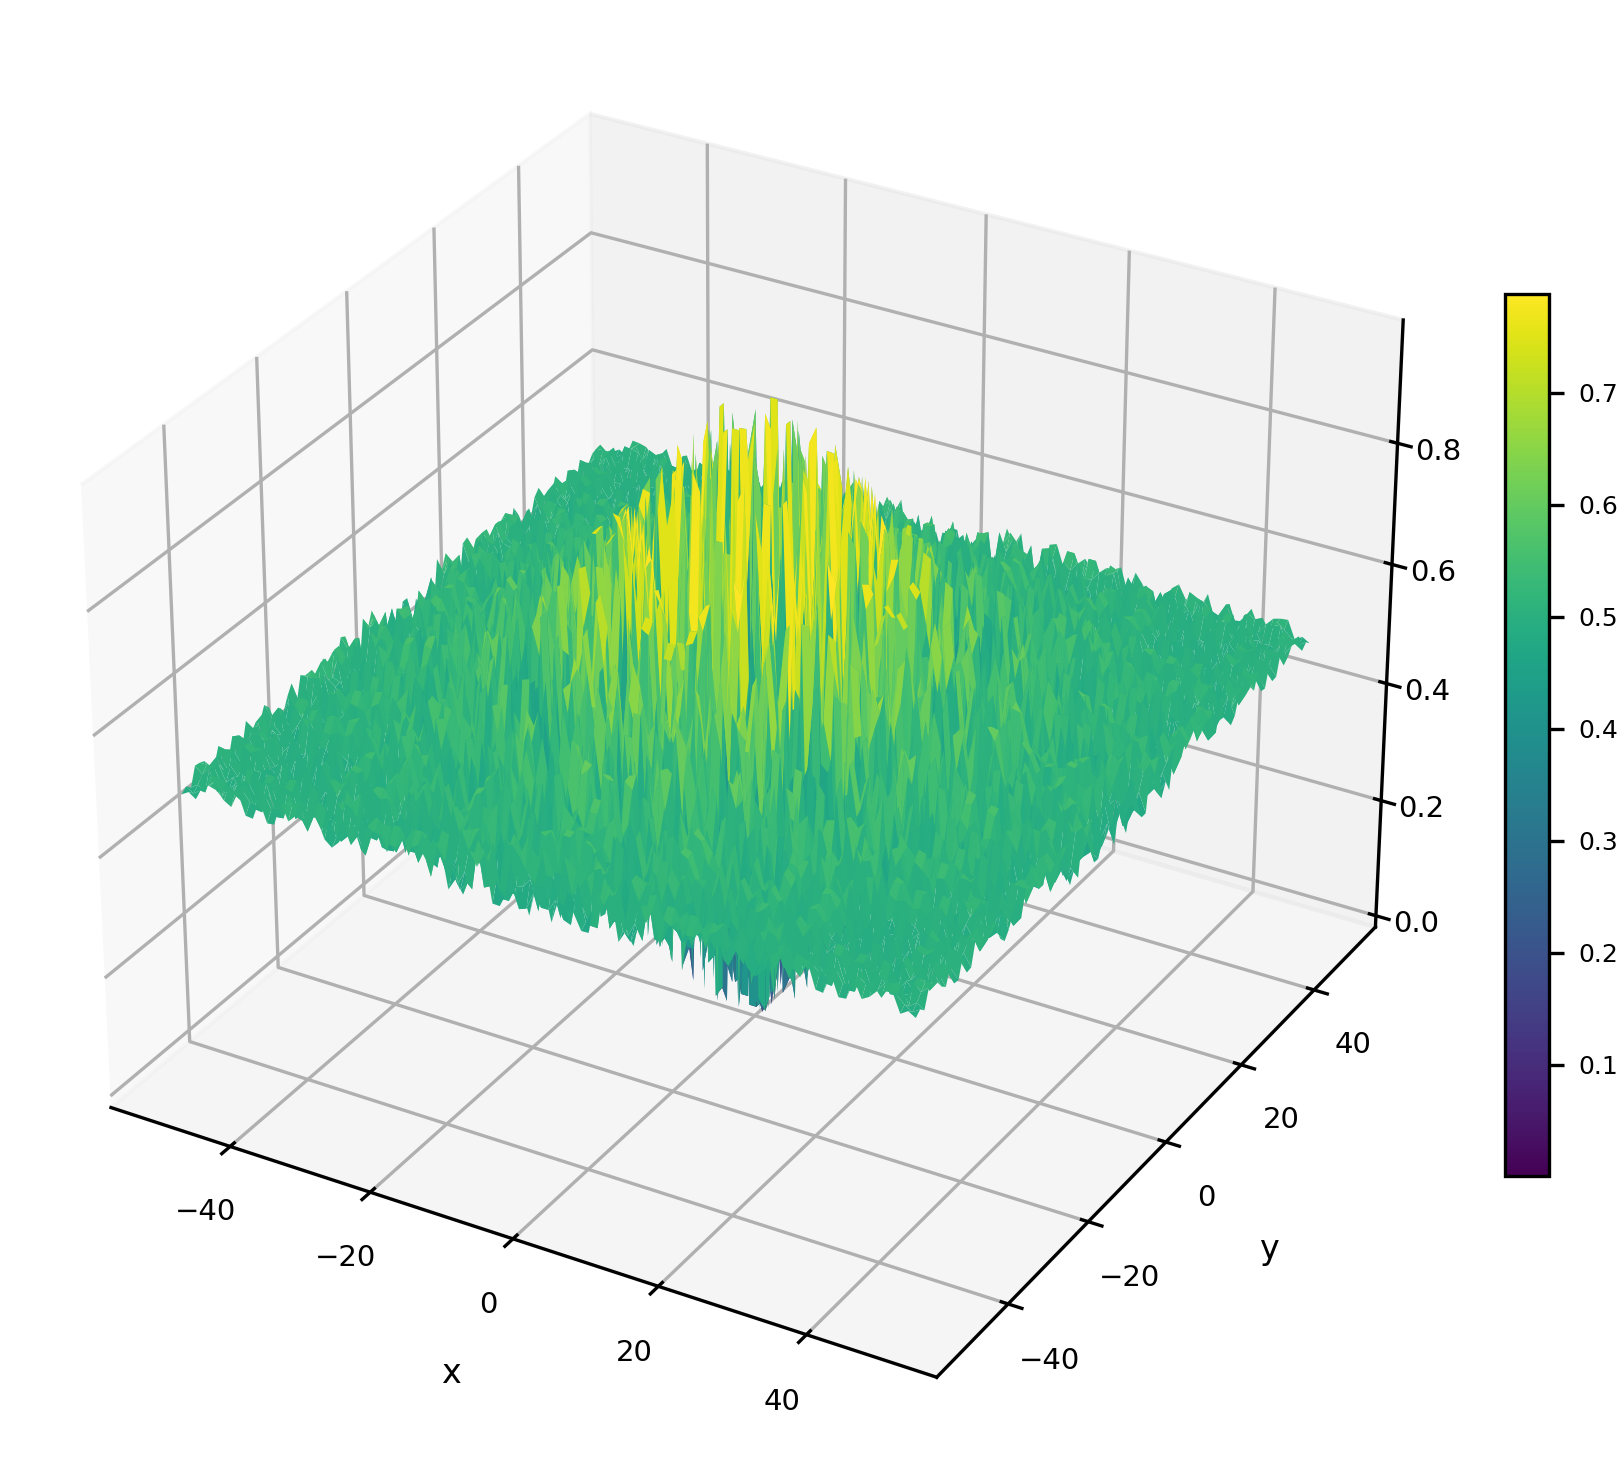
\includegraphics[width=1\textwidth]{Figures/benchmark_plots/Generalized_Schaffer_N1_maximized.png}
        \caption{Generalized Schaffer N1}
    \end{subfigure}
        \begin{subfigure}{0.32\textwidth}
        \centering
        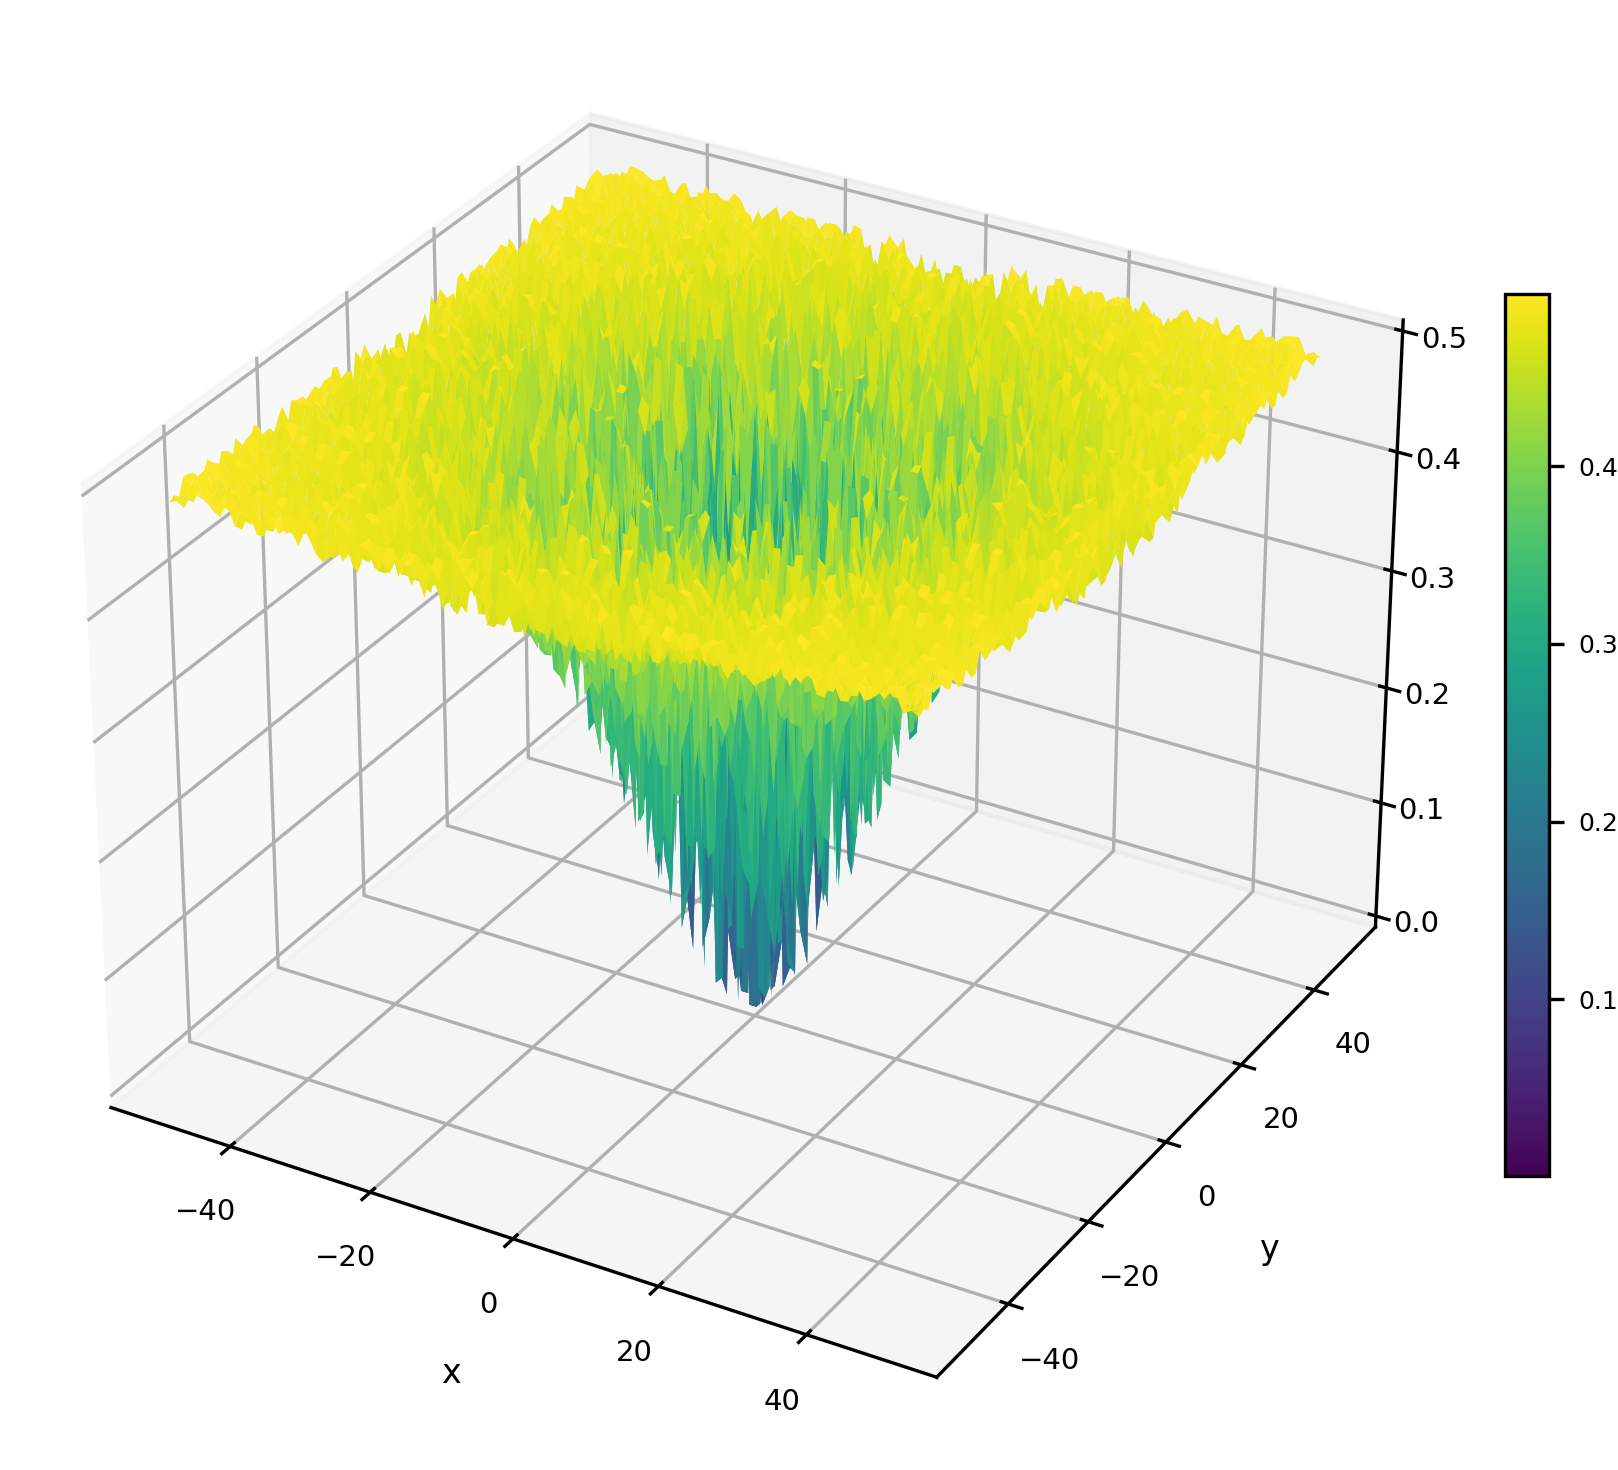
\includegraphics[width=1\textwidth]{Figures/benchmark_plots/Generalized_Schaffer_N2_maximized.png}
        \caption{Generalized Schaffer N2}
    \end{subfigure}
        \begin{subfigure}{0.32\textwidth}
        \centering
        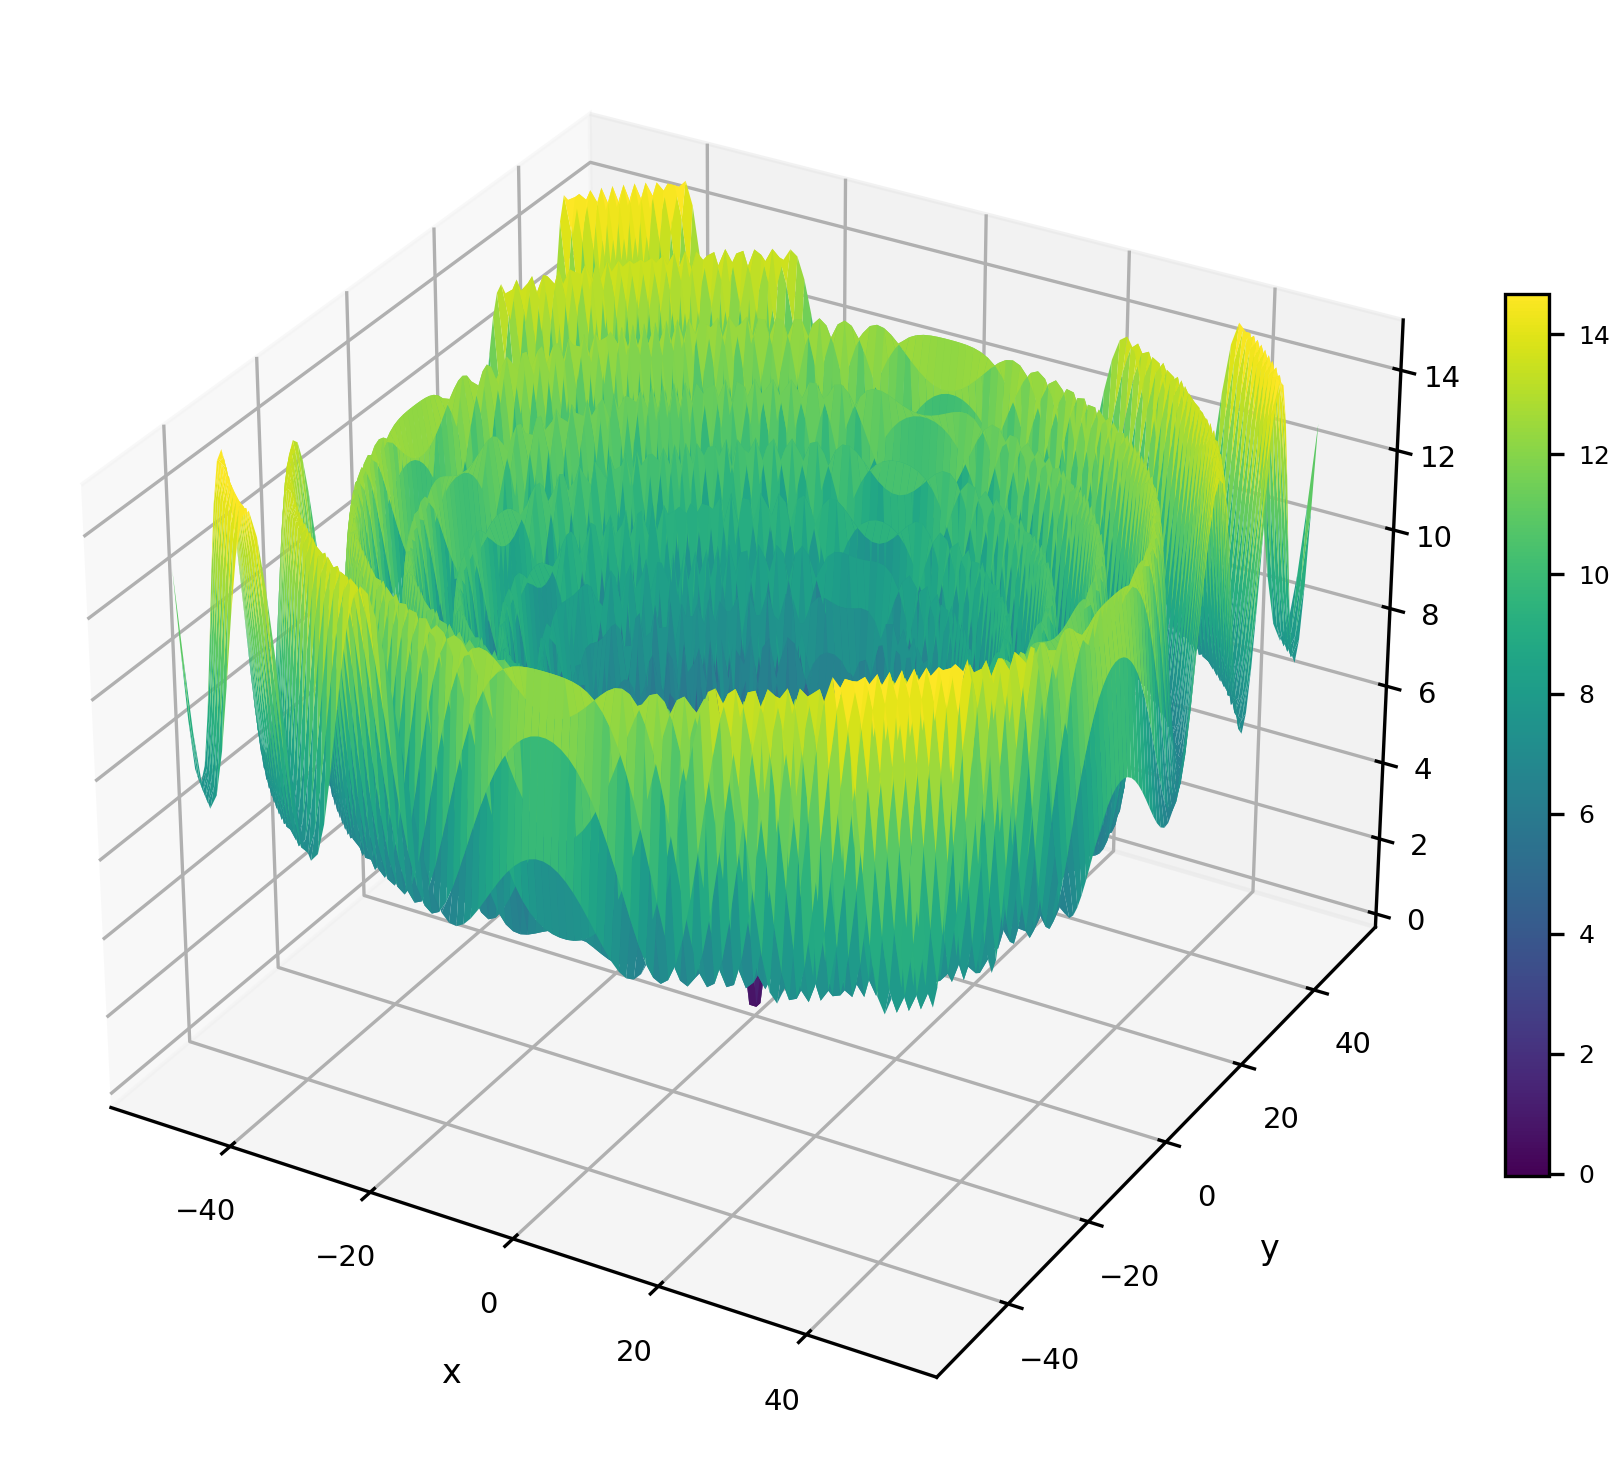
\includegraphics[width=1\textwidth]{Figures/benchmark_plots/Generalized_Schaffer_N3_maximized.png}
        \caption{Generalized Schaffer N3}
    \end{subfigure}
      \begin{subfigure}{0.32\textwidth}
        \centering
        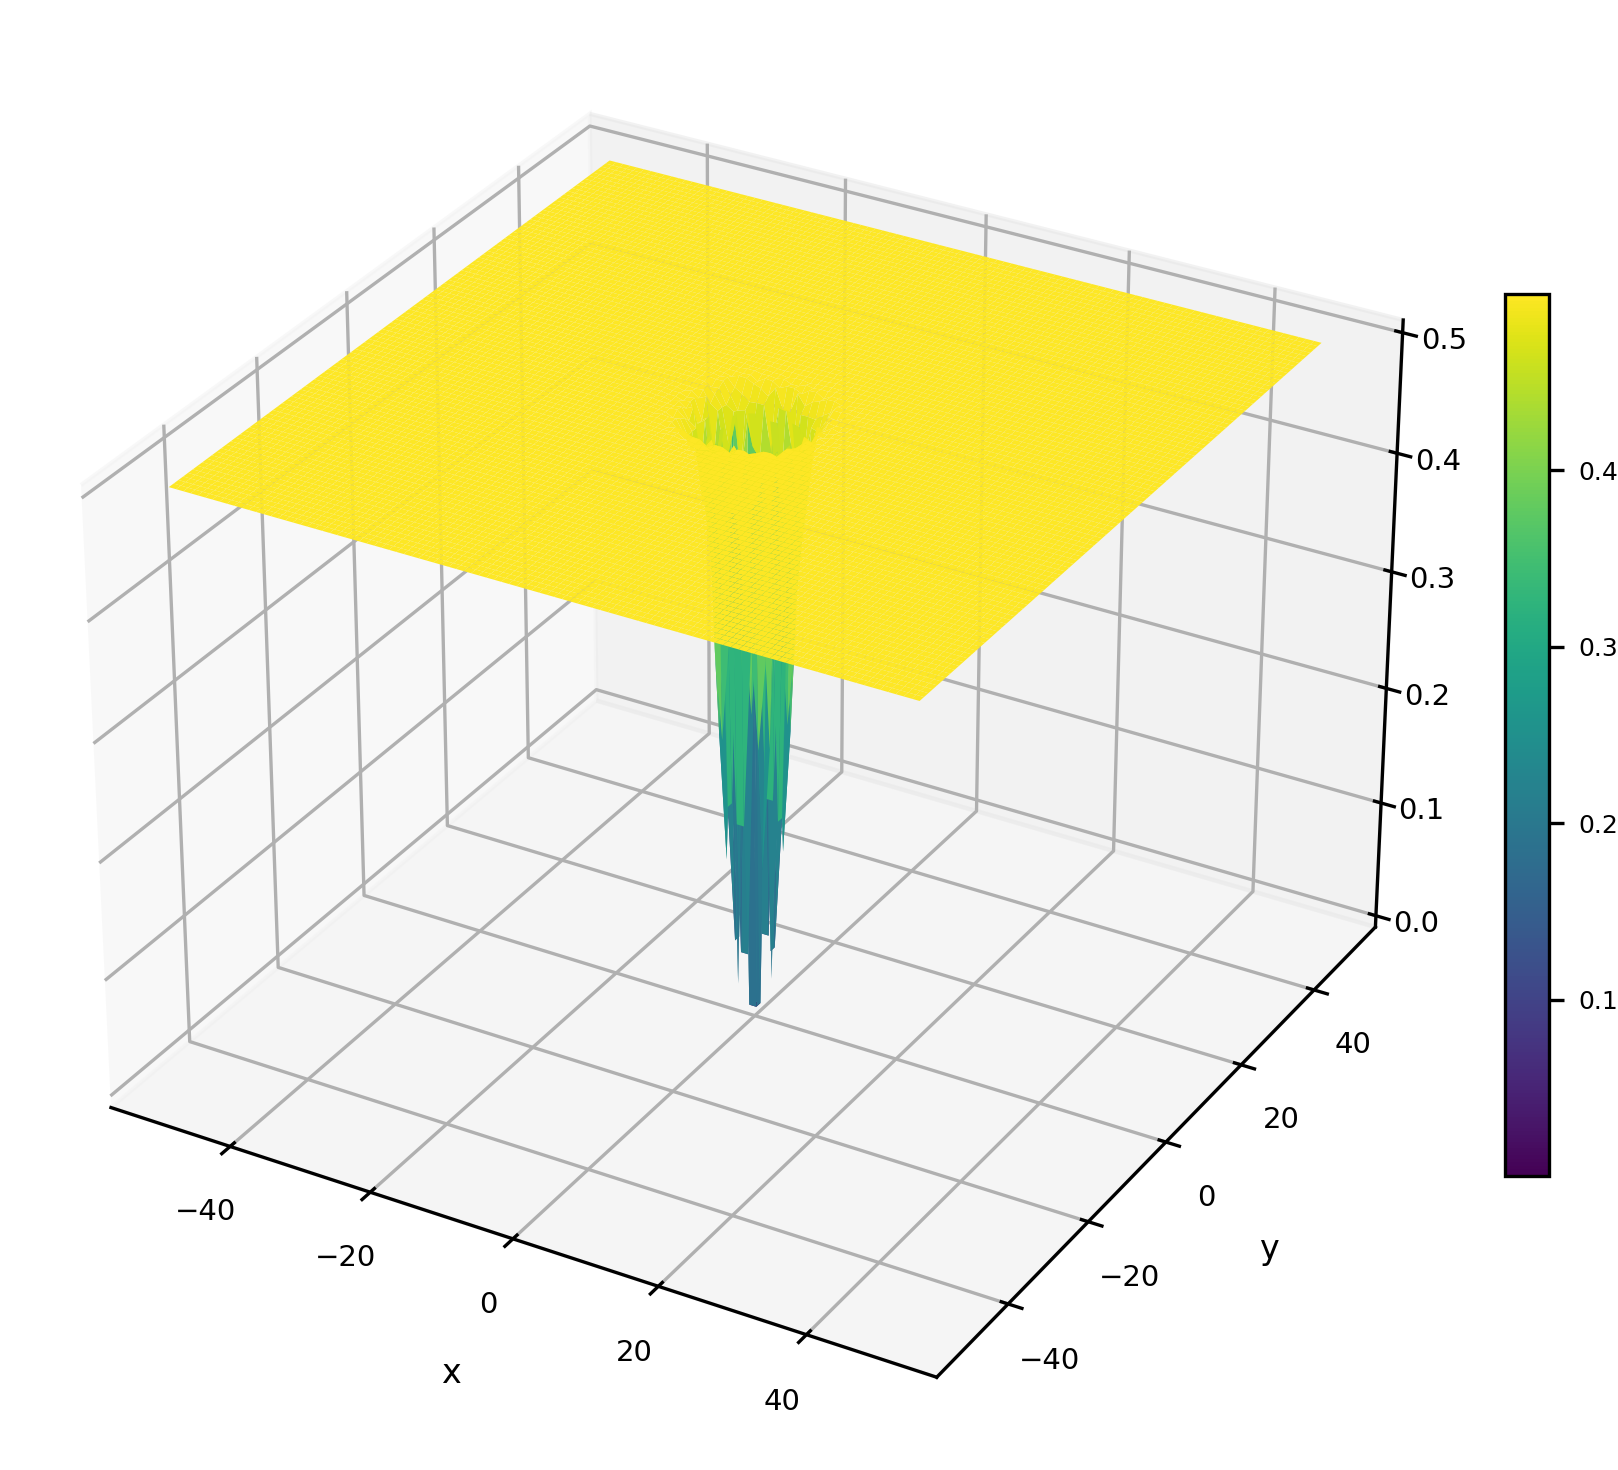
\includegraphics[width=1\textwidth]{Figures/benchmark_plots/Generalized_Schaffer_N4_maximized.png}
        \caption{Generalized Schaffer N4}
    \end{subfigure}
        \begin{subfigure}{0.32\textwidth}
        \centering
        \includegraphics[width=1\textwidth]{Figures/benchmark_plots/Generalized_Schmidt–Vetters_maximized.png}
        \caption{Schmidt–Vetters}
    \end{subfigure}
    \caption[Visualizations of benchmark problem landscapes]{Two-dimensional visualizations of benchmark problem landscapes.}
\end{figure}


\begin{figure}[p]\ContinuedFloat
\renewcommand\thesubfigure{A.\arabic{subfigure}} % Local change starts here
    \centering
    \begin{subfigure}{0.32\textwidth}
        \centering
        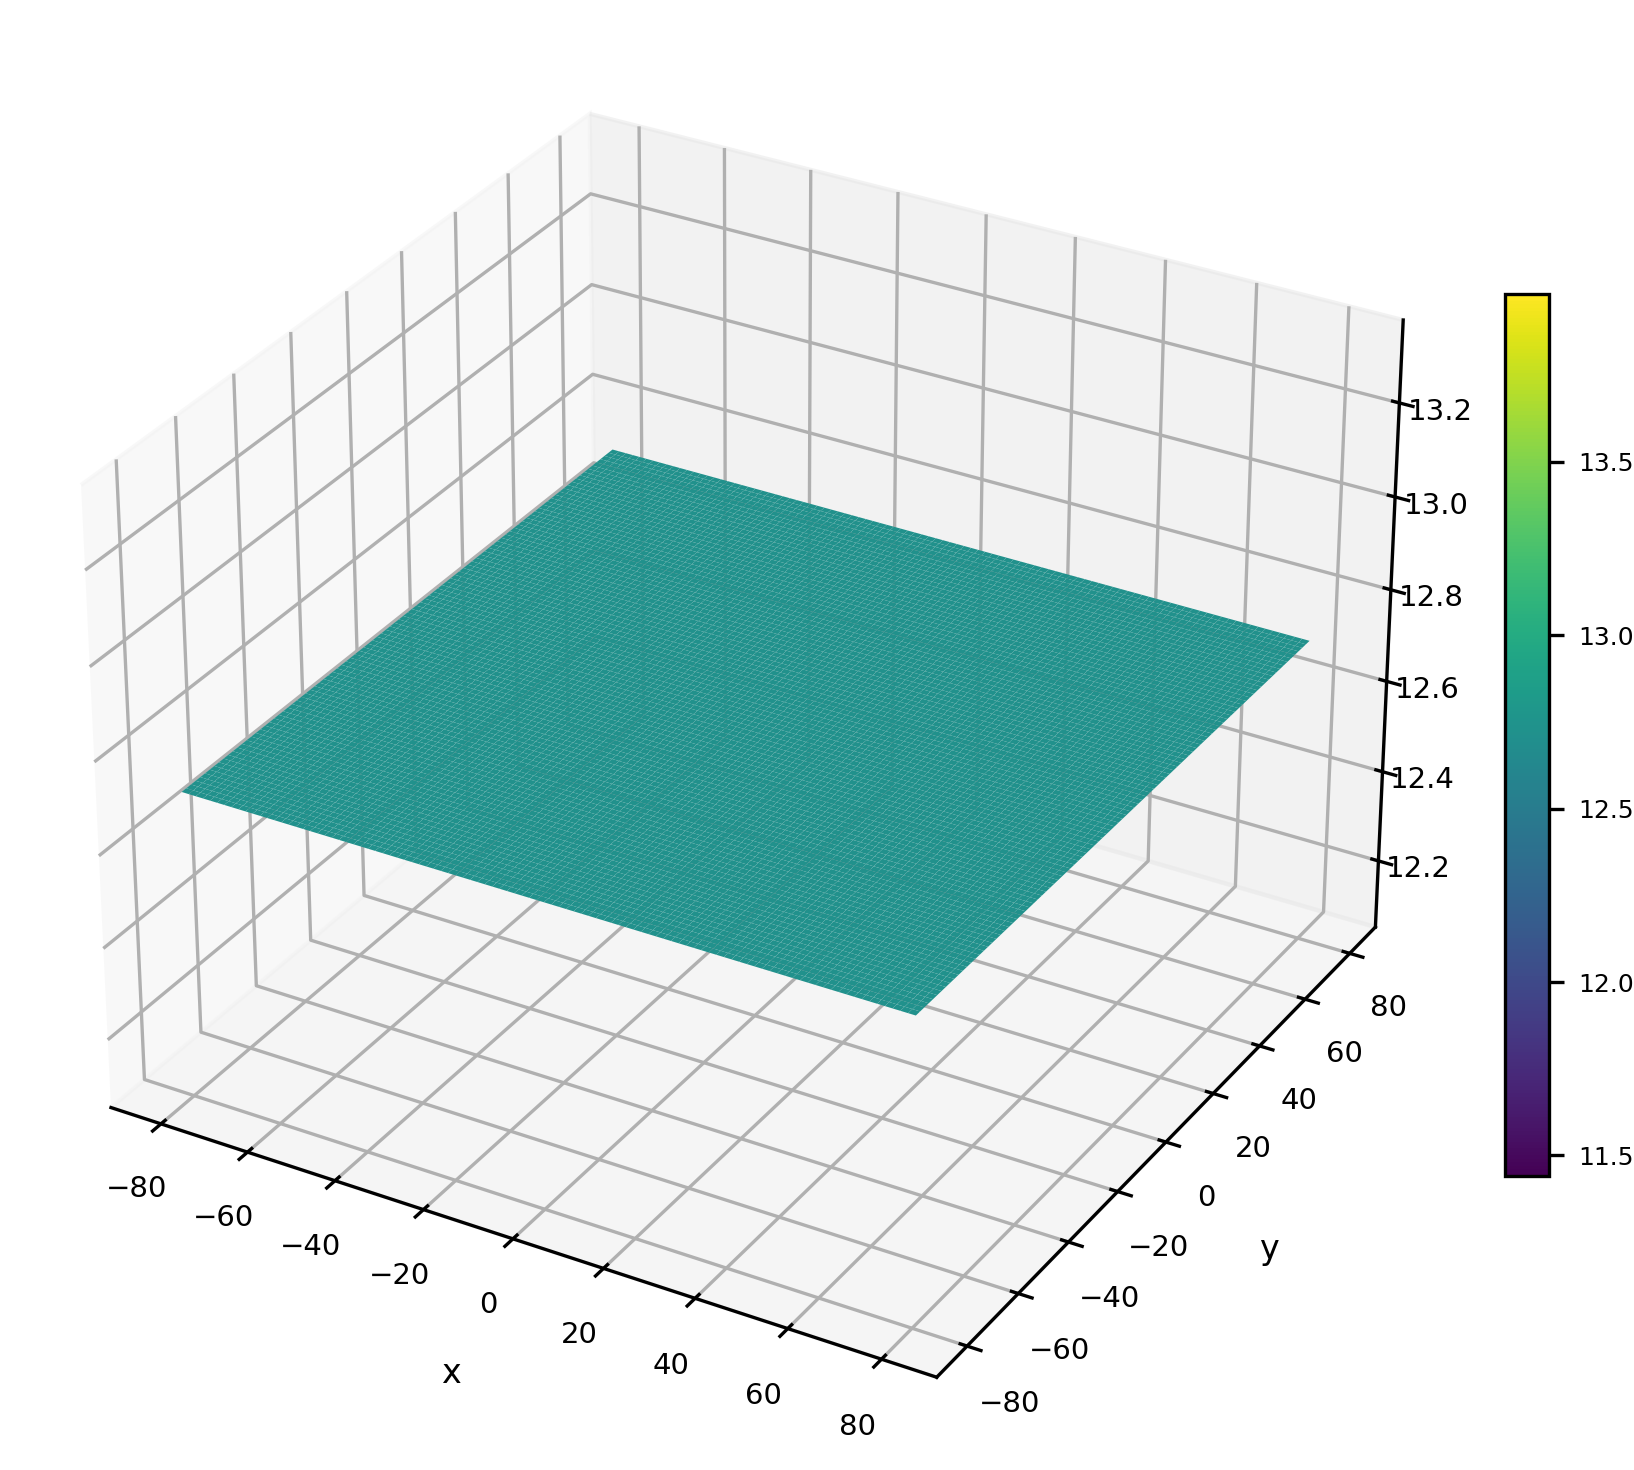
\includegraphics[width=1\textwidth]{Figures/benchmark_plots/Lennard_Jones_Minimum_Energy_Cluster_maximized.png}
        \caption{Lennard‑Jones}
    \end{subfigure}
    \begin{subfigure}{0.32\textwidth}
        \centering
        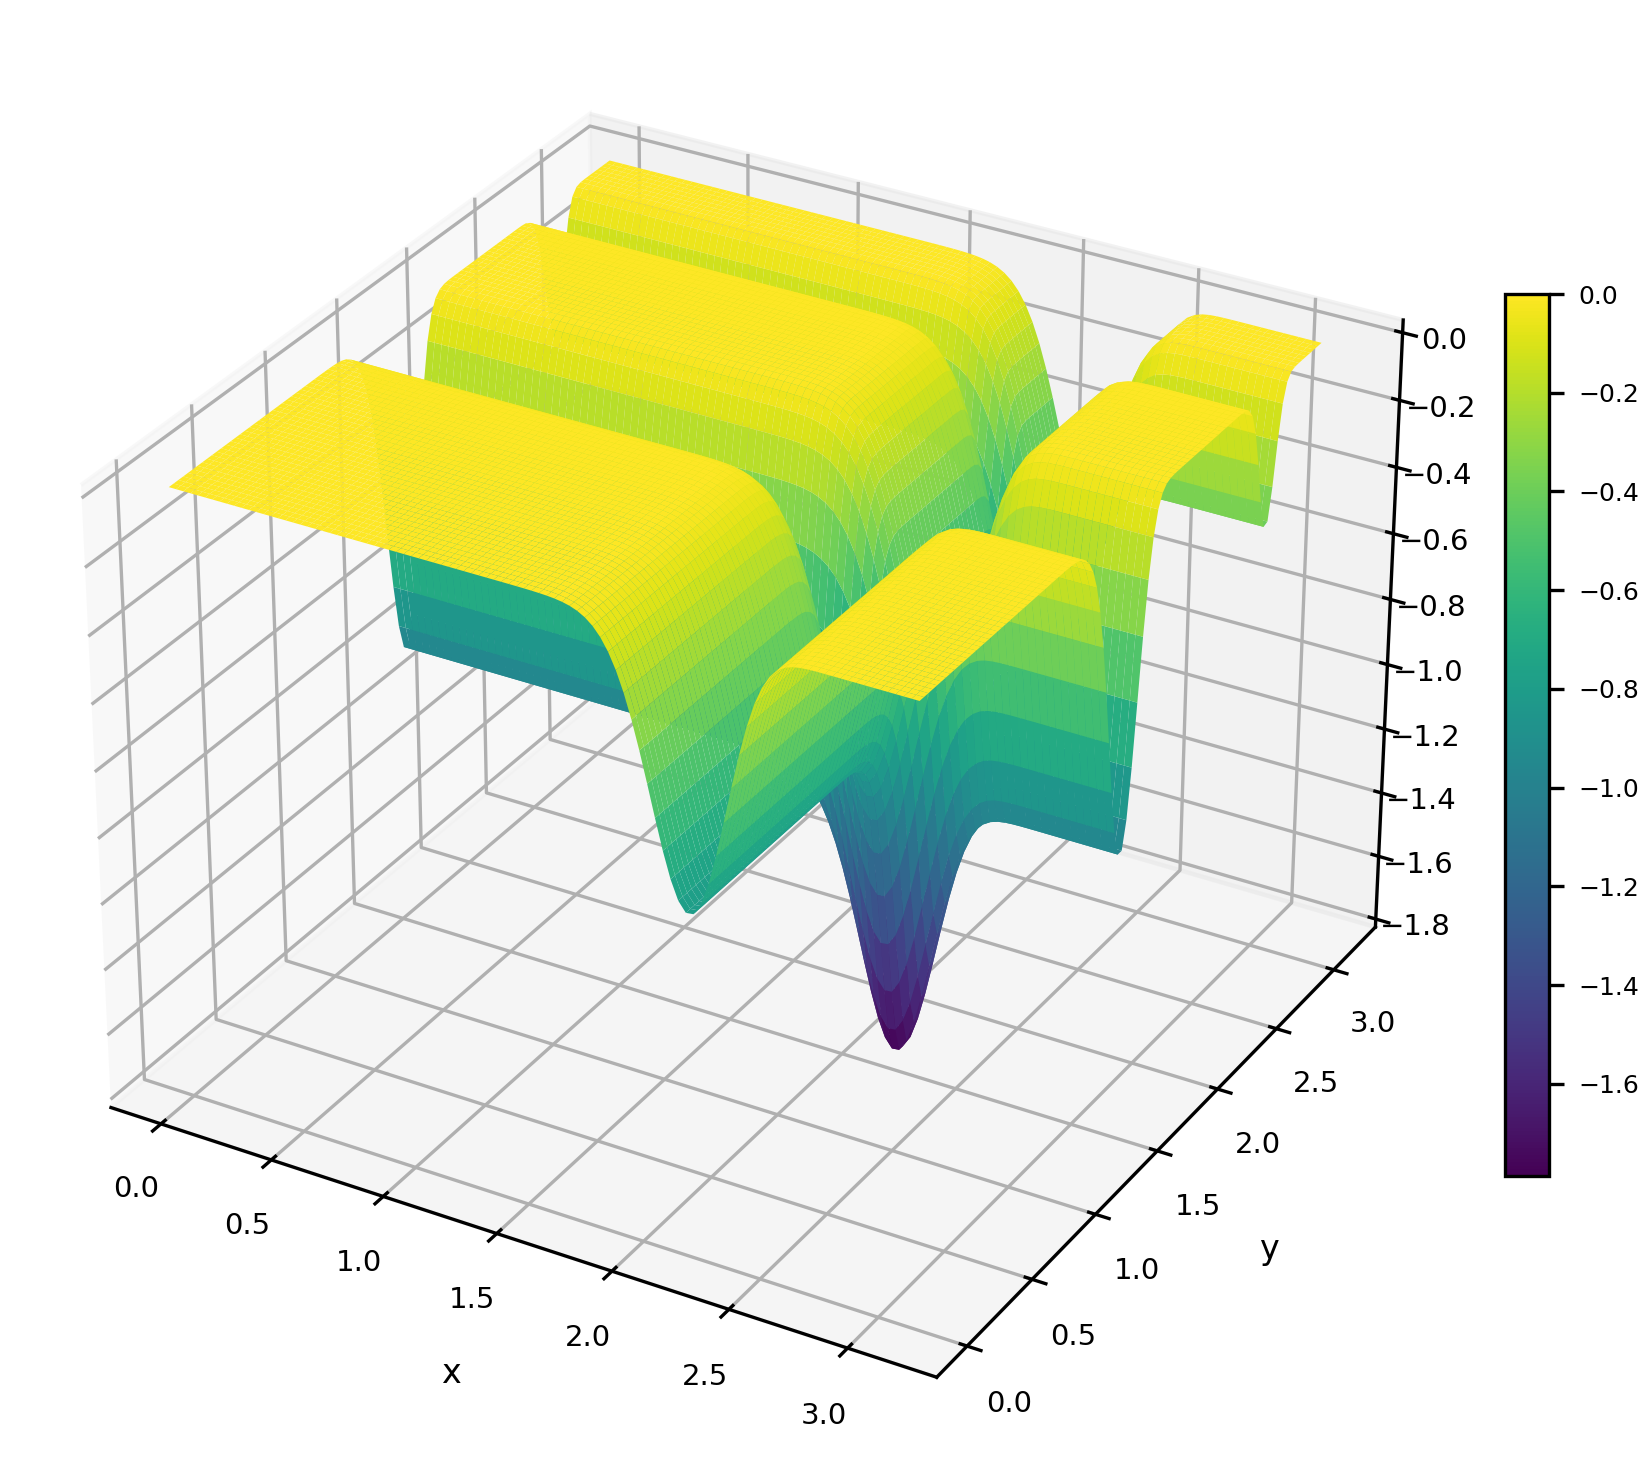
\includegraphics[width=1\textwidth]{Figures/benchmark_plots/Michalewicz_maximized.png}
        \caption{Michalewicz}
    \end{subfigure}
    % \hspace{.5cm} % Adjust the space as needed.
    \begin{subfigure}{0.32\textwidth}
        \centering
        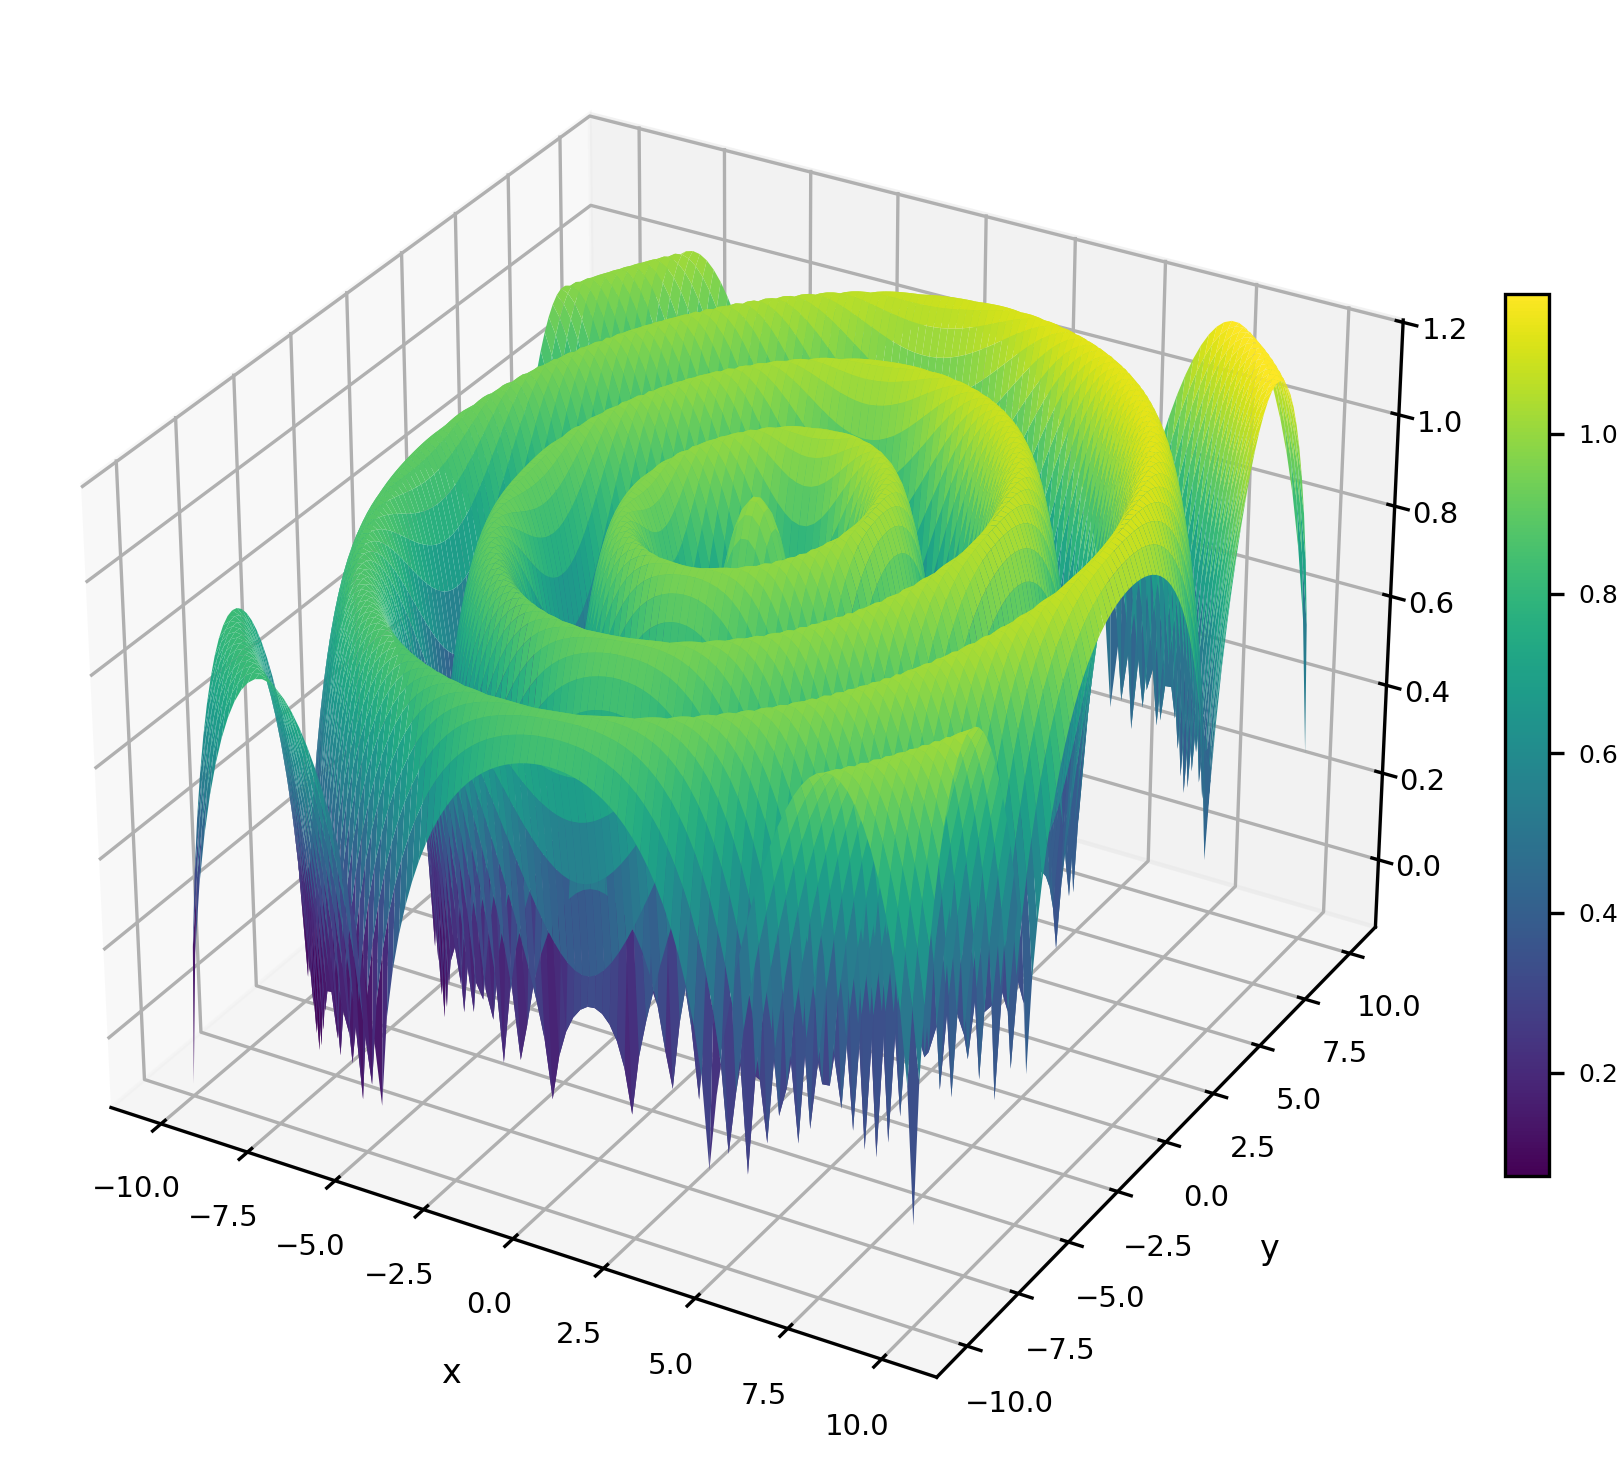
\includegraphics[width=1\textwidth]{Figures/benchmark_plots/Mishra_N3_maximized.png}
        \caption{Mishra 03}
    \end{subfigure}
    \begin{subfigure}{0.48\textwidth}
        \centering
        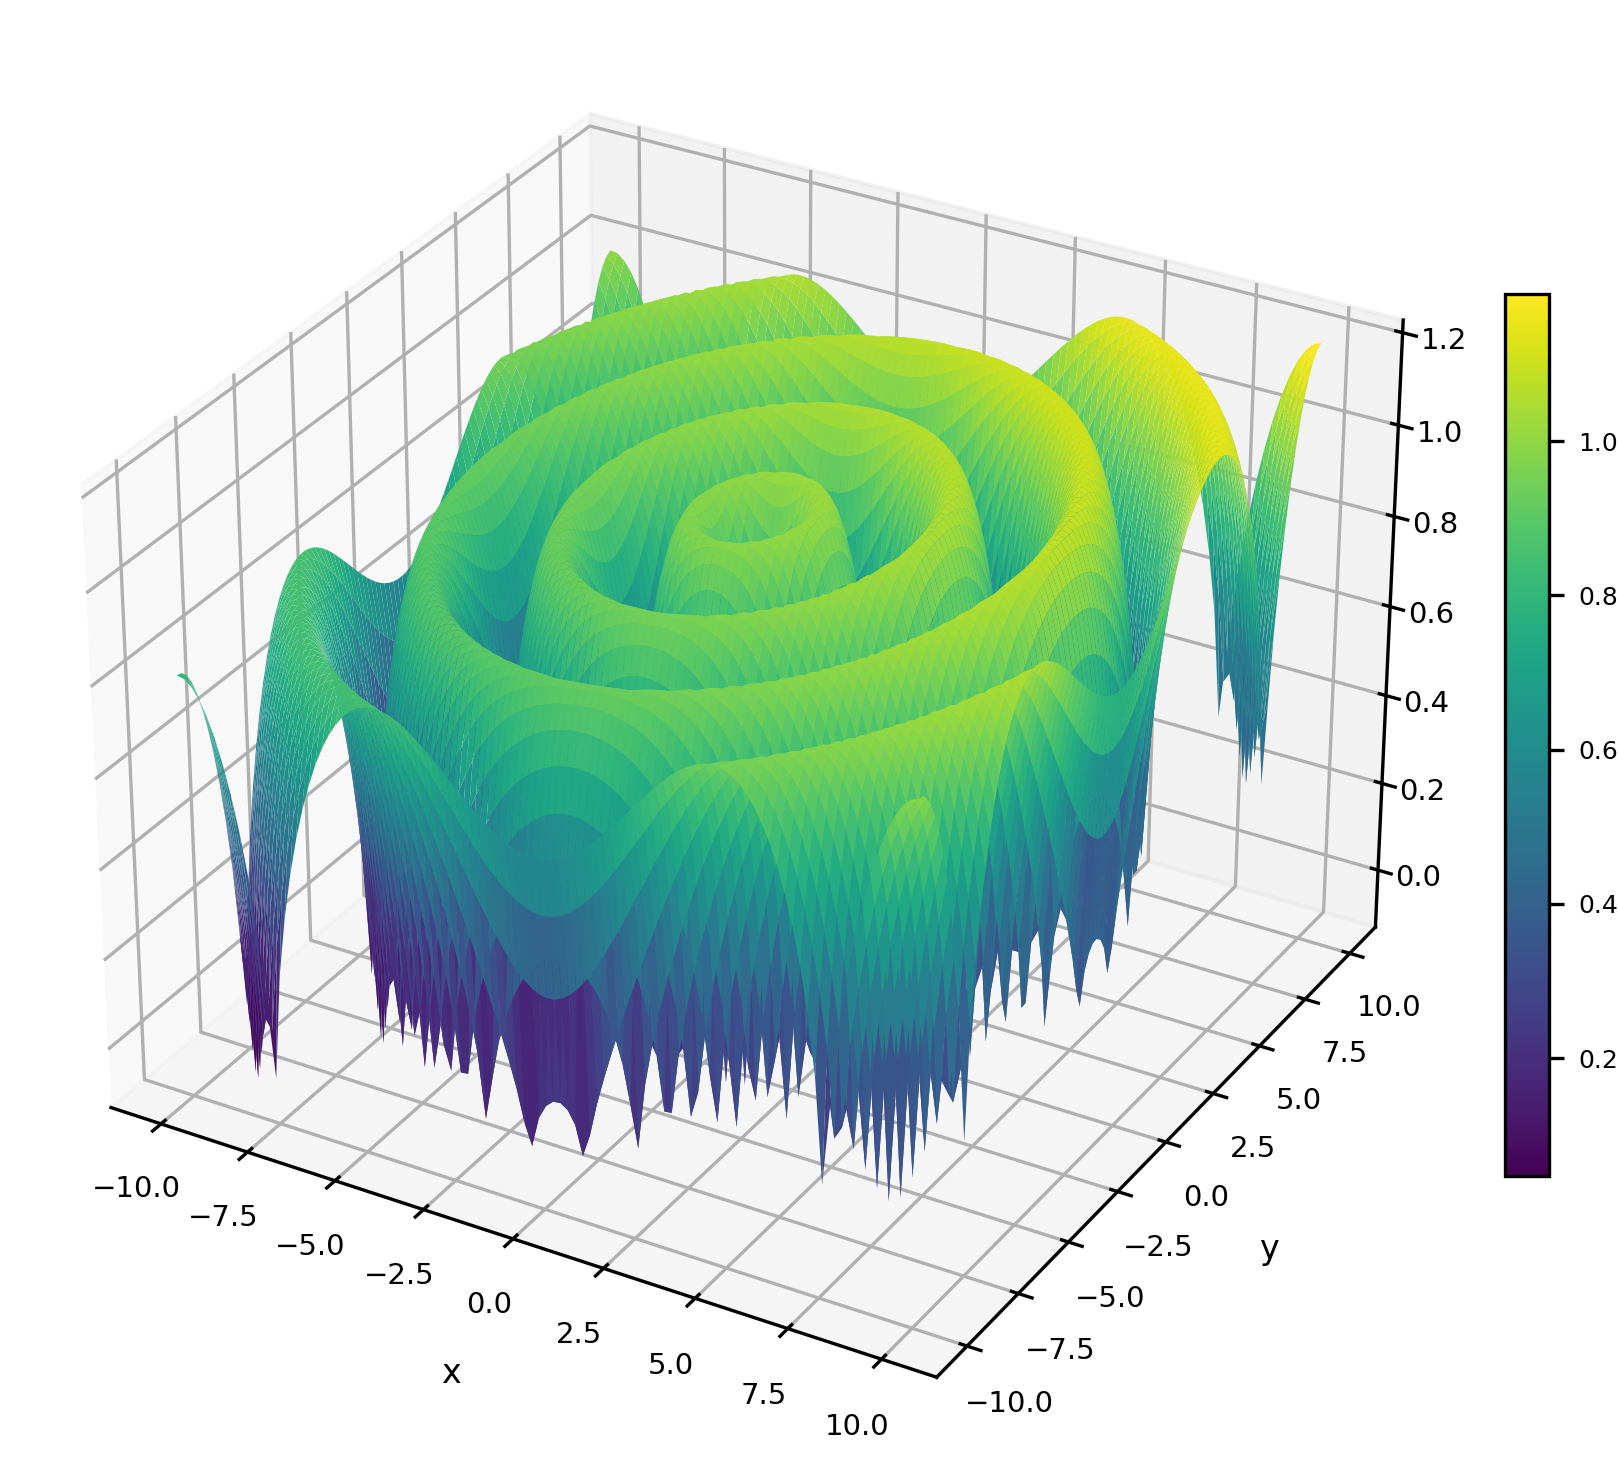
\includegraphics[width=1\textwidth]{Figures/benchmark_plots/Mishra_N4_maximized.png}
        \caption{Mishra 04}
    \end{subfigure}
    % \hspace{.5cm} % Adjust the space as needed.
    \begin{subfigure}{0.48\textwidth}
        \centering
        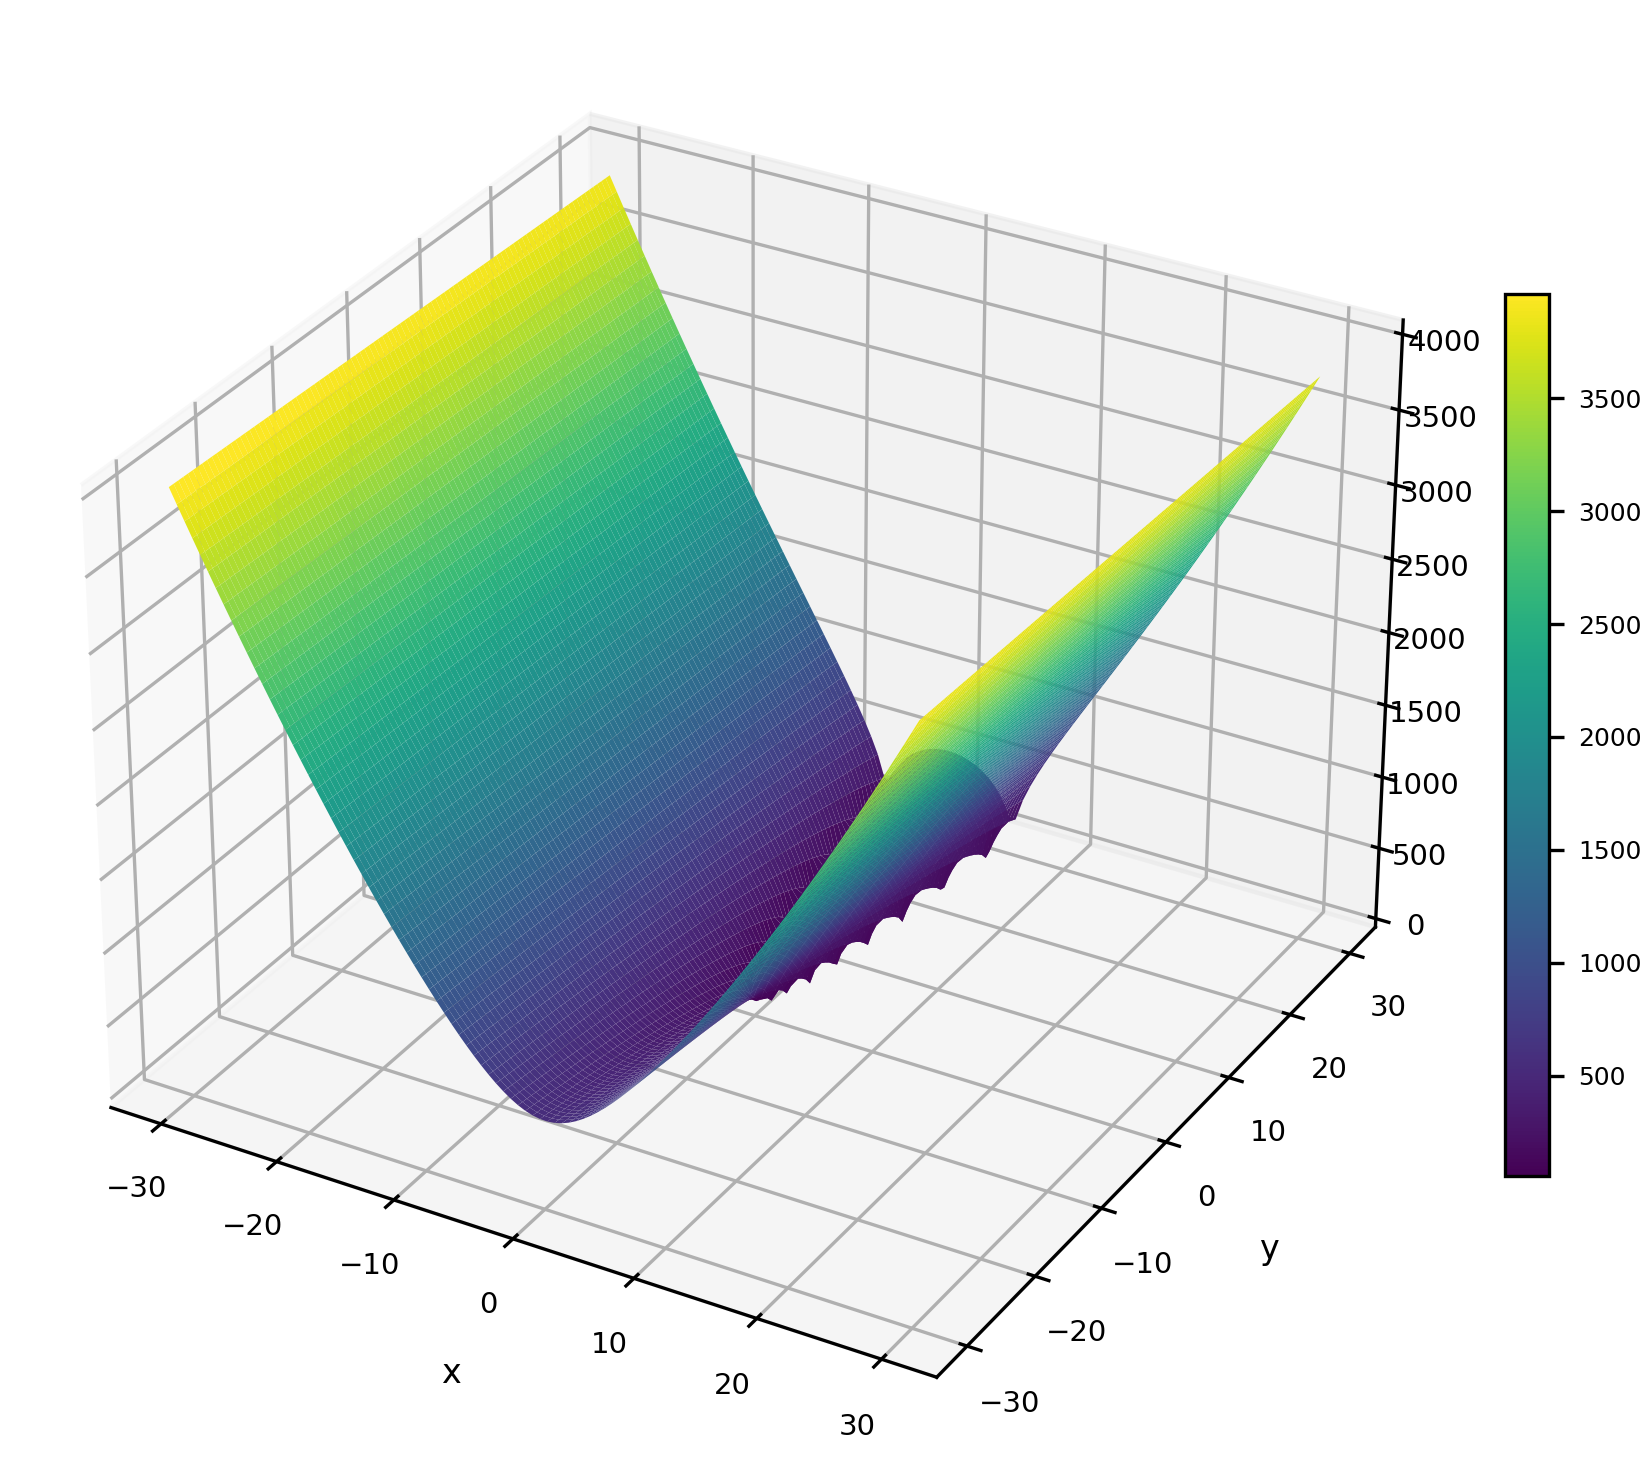
\includegraphics[width=1\textwidth]{Figures/benchmark_plots/Modified_Rosenbrock_No.02___Hollow_Ground_Bent_Knife_Edge_maximized.png}
        \caption{Modified Rosenbrock N.2}
    \end{subfigure}
    \begin{subfigure}{0.32\textwidth}
        \centering
        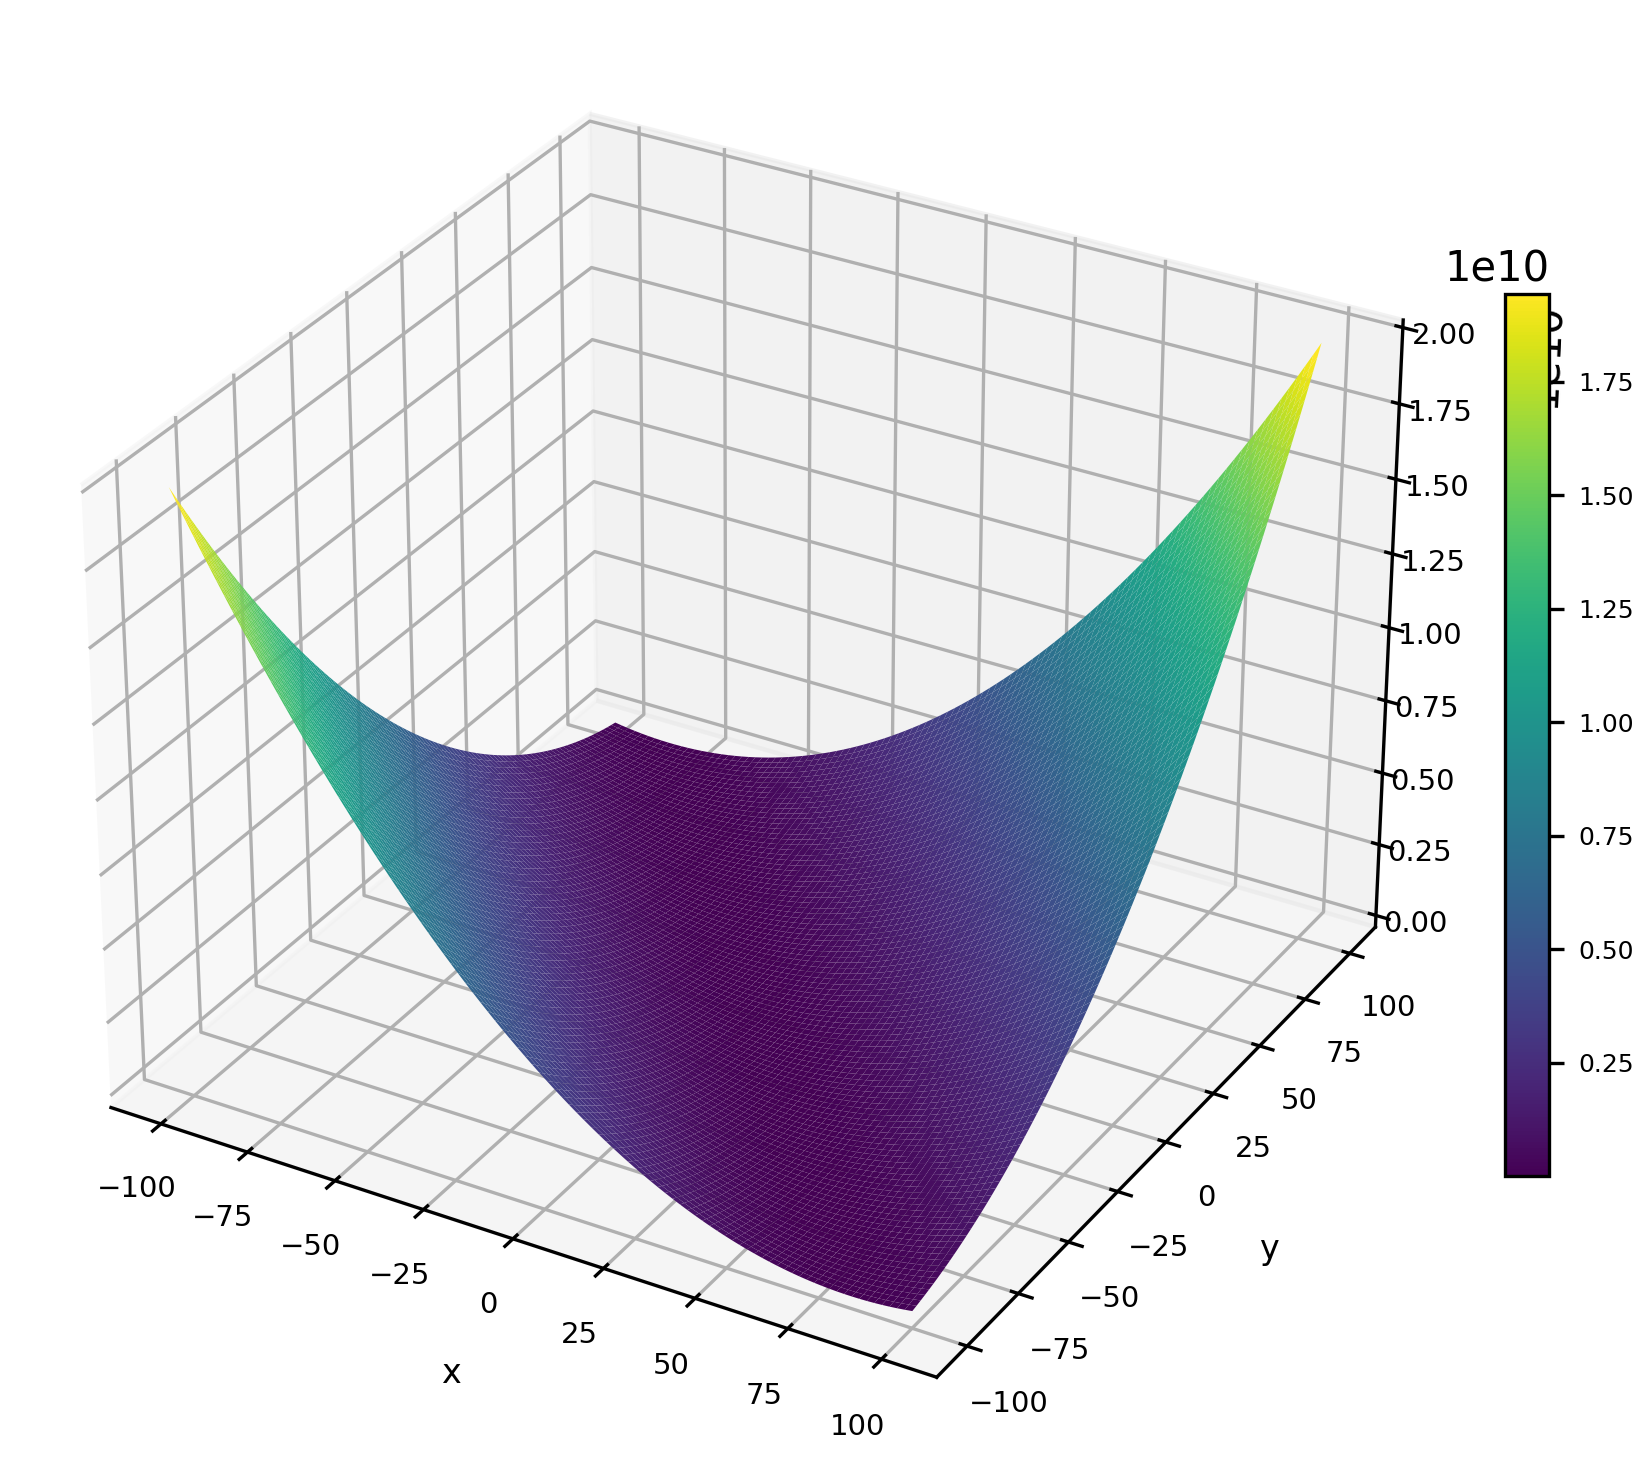
\includegraphics[width=1\textwidth]{Figures/benchmark_plots/Rotated_Bent_Cigar_maximized.png}
        \caption{Rotated Bent Cigar}
    \end{subfigure}
    % \hspace{.5cm} % Adjust the space as needed.
    \begin{subfigure}{0.32\textwidth}
        \centering
        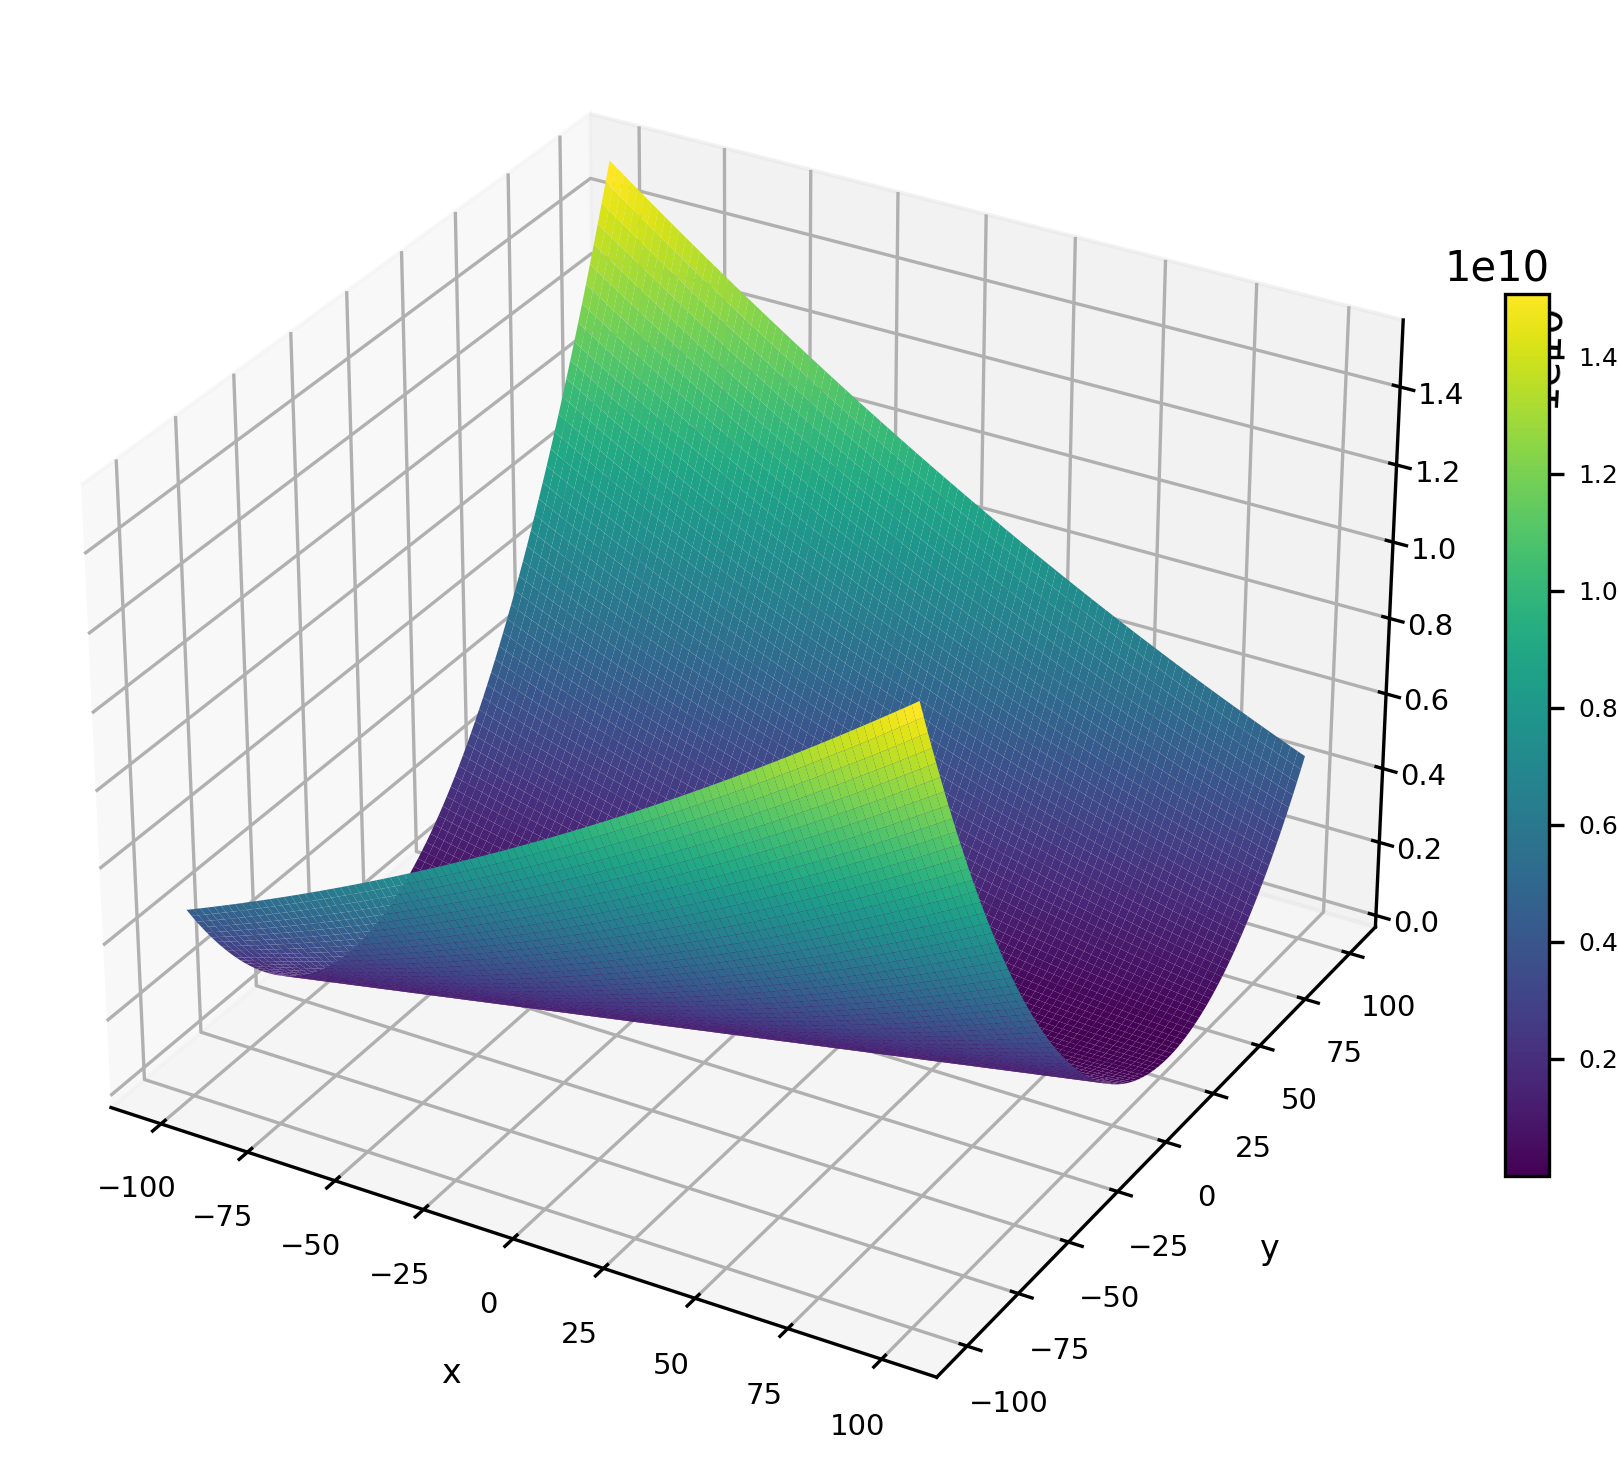
\includegraphics[width=1\textwidth]{Figures/benchmark_plots/Rotated_Discus_maximized.png}
        \caption{Rotated Discus}
    \end{subfigure}
        \begin{subfigure}{0.32\textwidth}
        \centering
        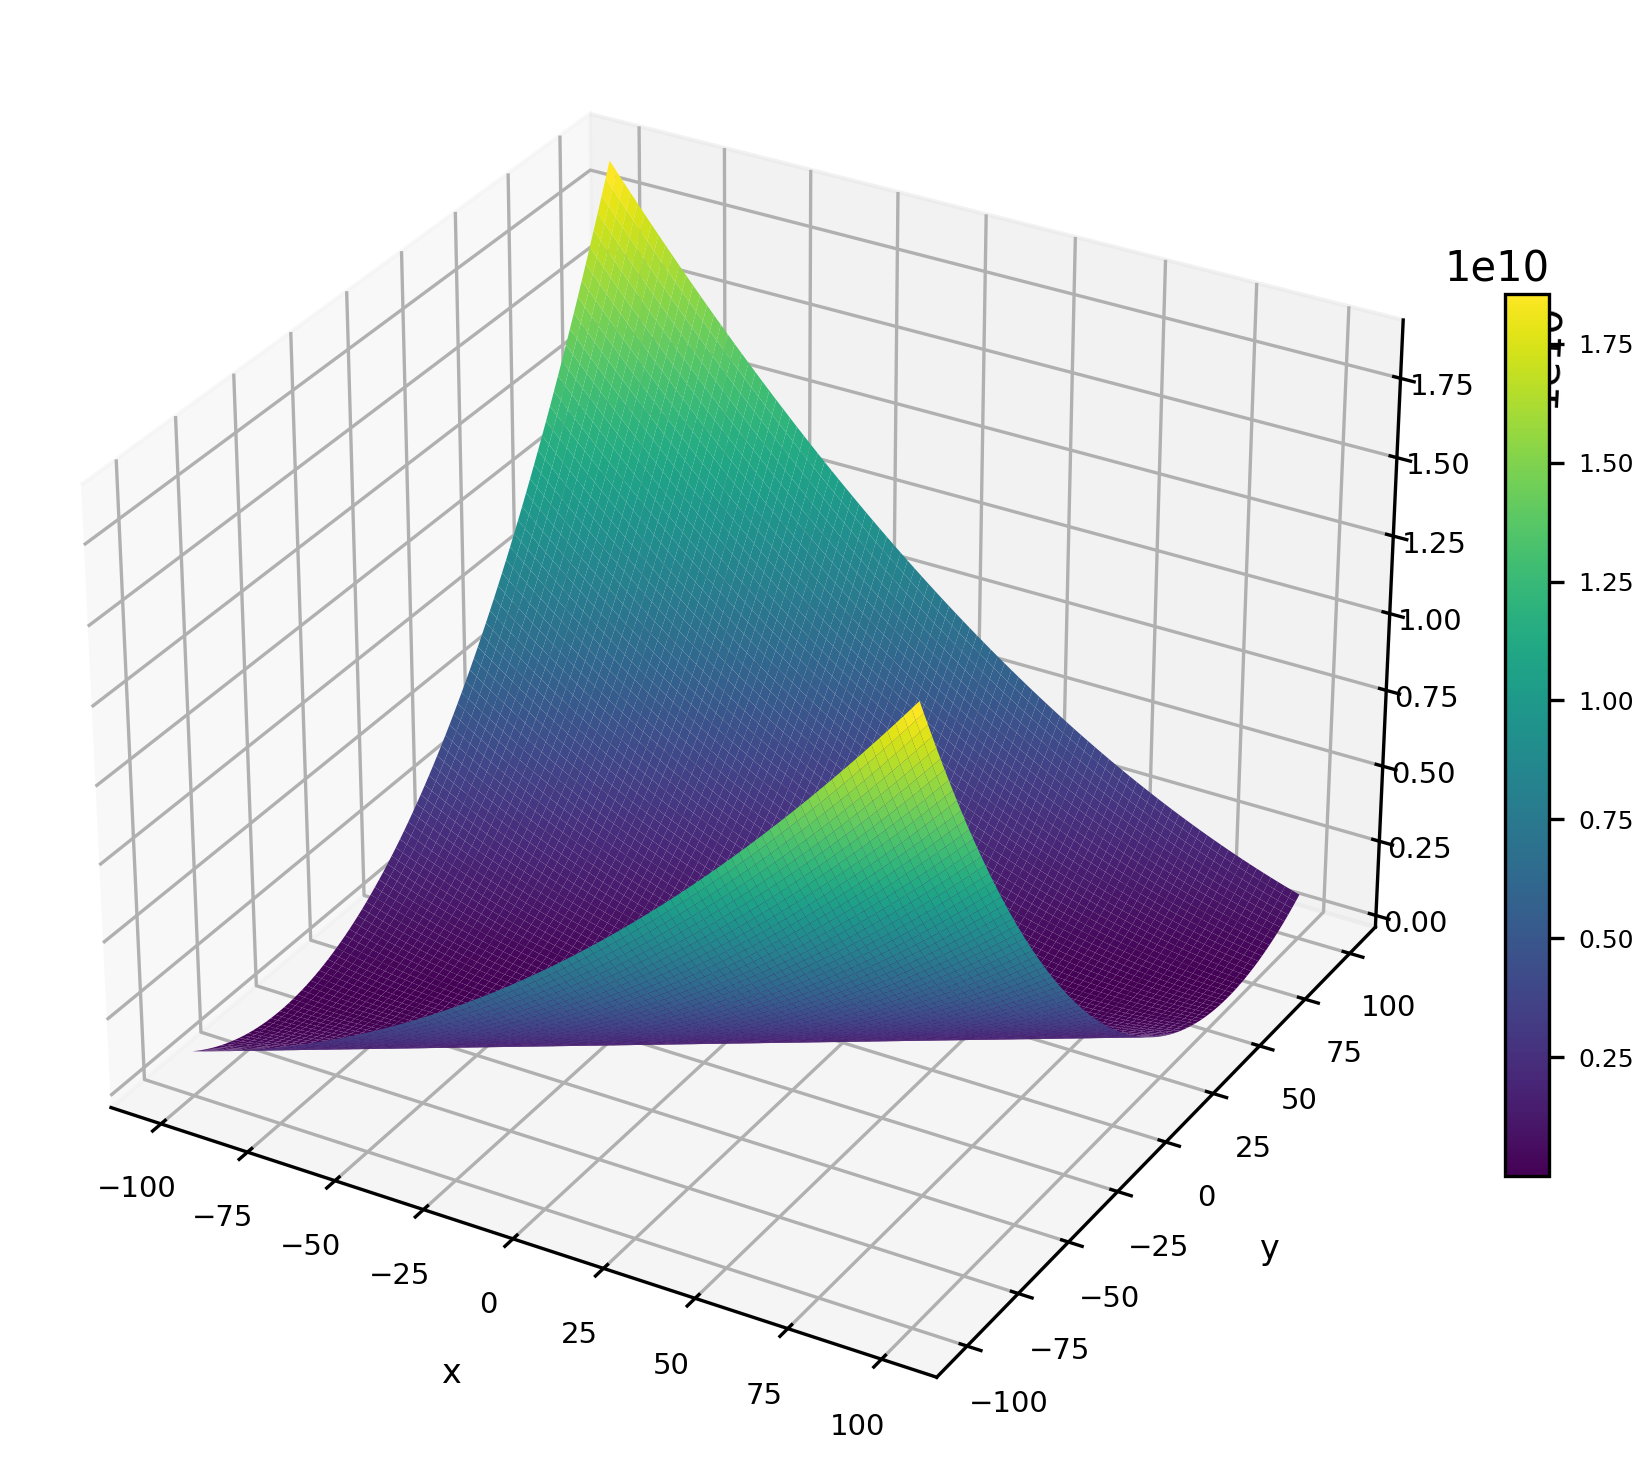
\includegraphics[width=1\textwidth]{Figures/benchmark_plots/Rotated_High_Conditioned_Elliptic_maximized.png}
        \caption{Rotated Elliptic}
    \end{subfigure}
    % \hspace{.5cm} % Adjust the space as needed.
    \begin{subfigure}{0.32\textwidth}
        \centering
        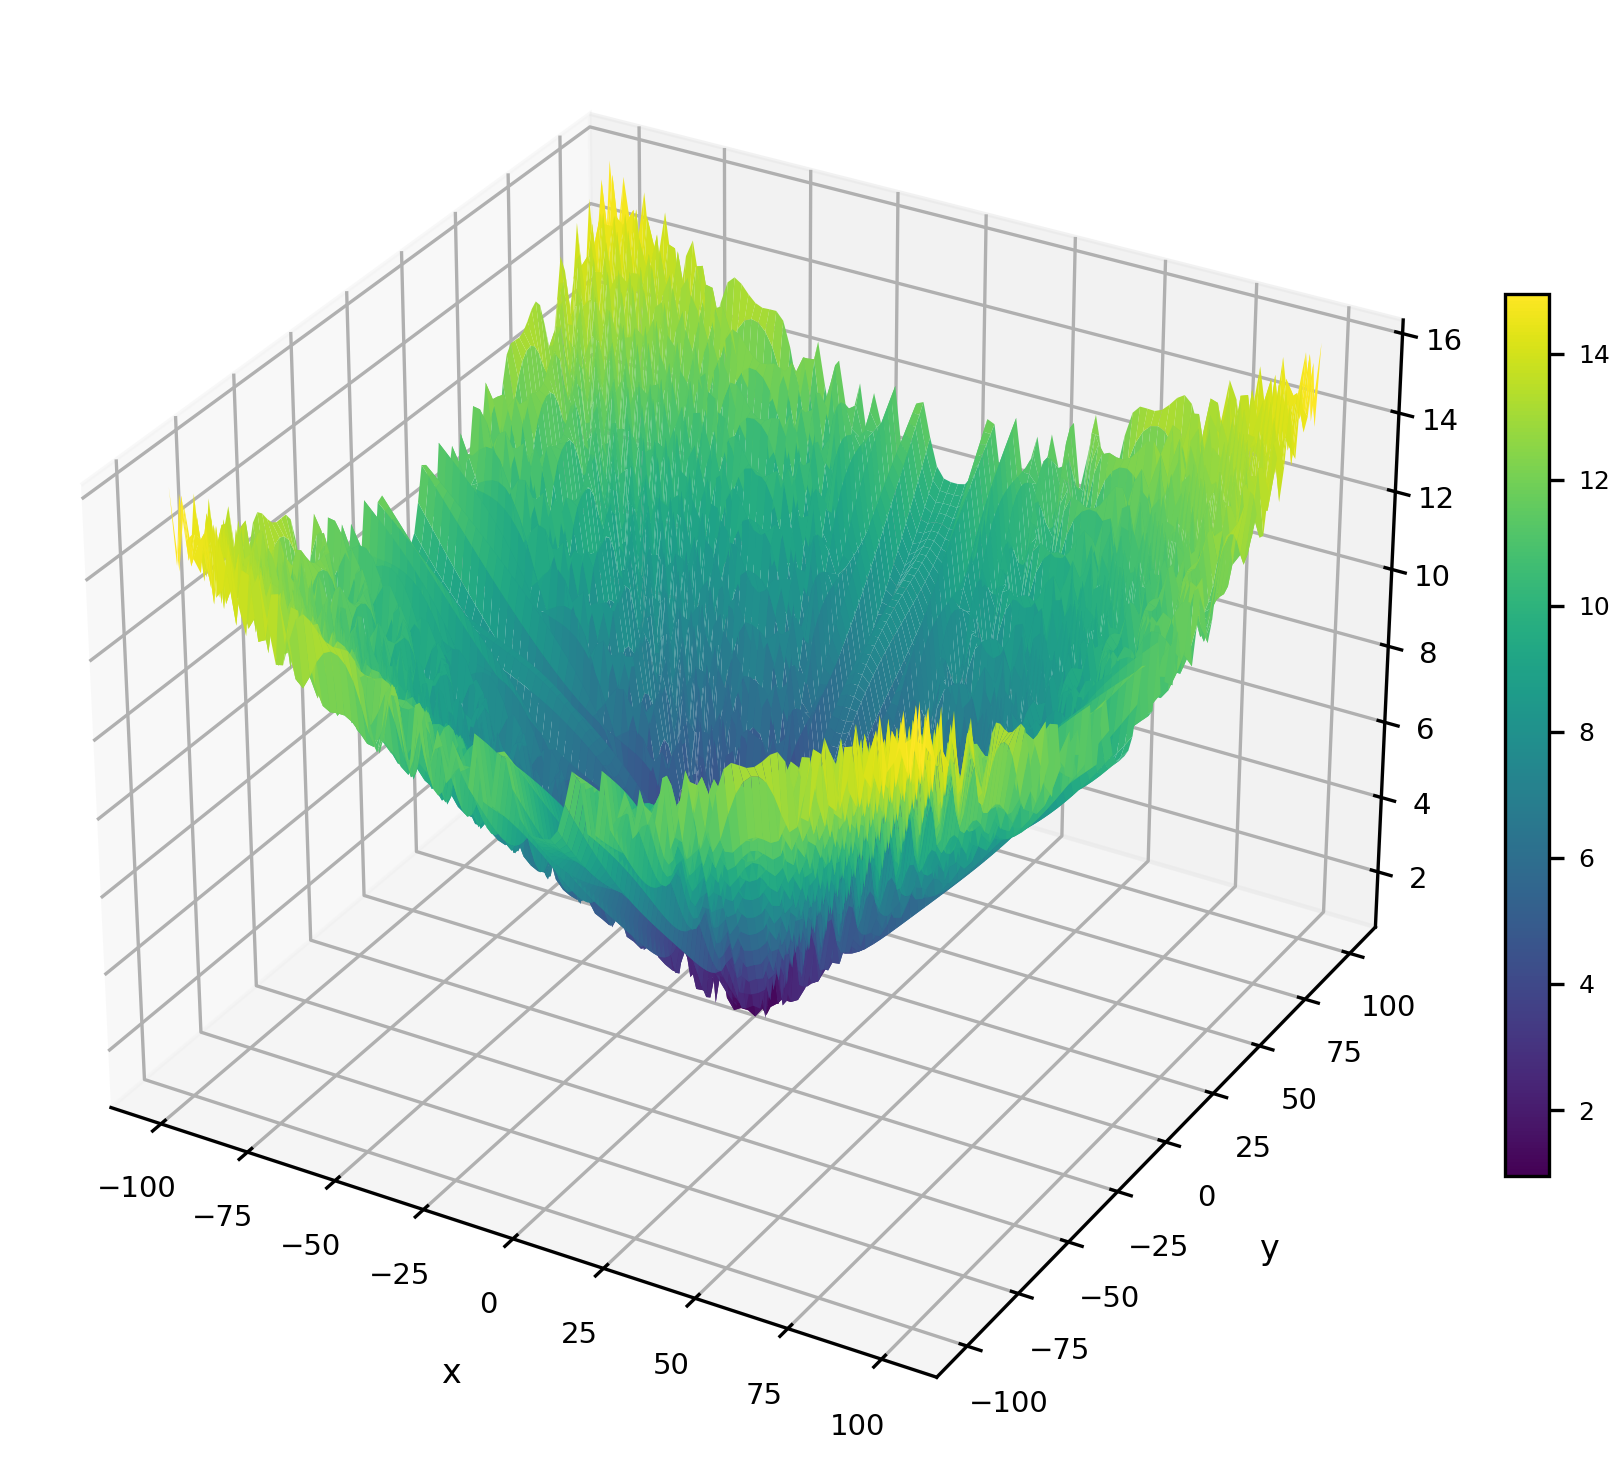
\includegraphics[width=1\textwidth]{Figures/benchmark_plots/Salomon_maximized.png}
        \caption{Salomon}
    \end{subfigure}
    \begin{subfigure}{0.32\textwidth}
        \centering
        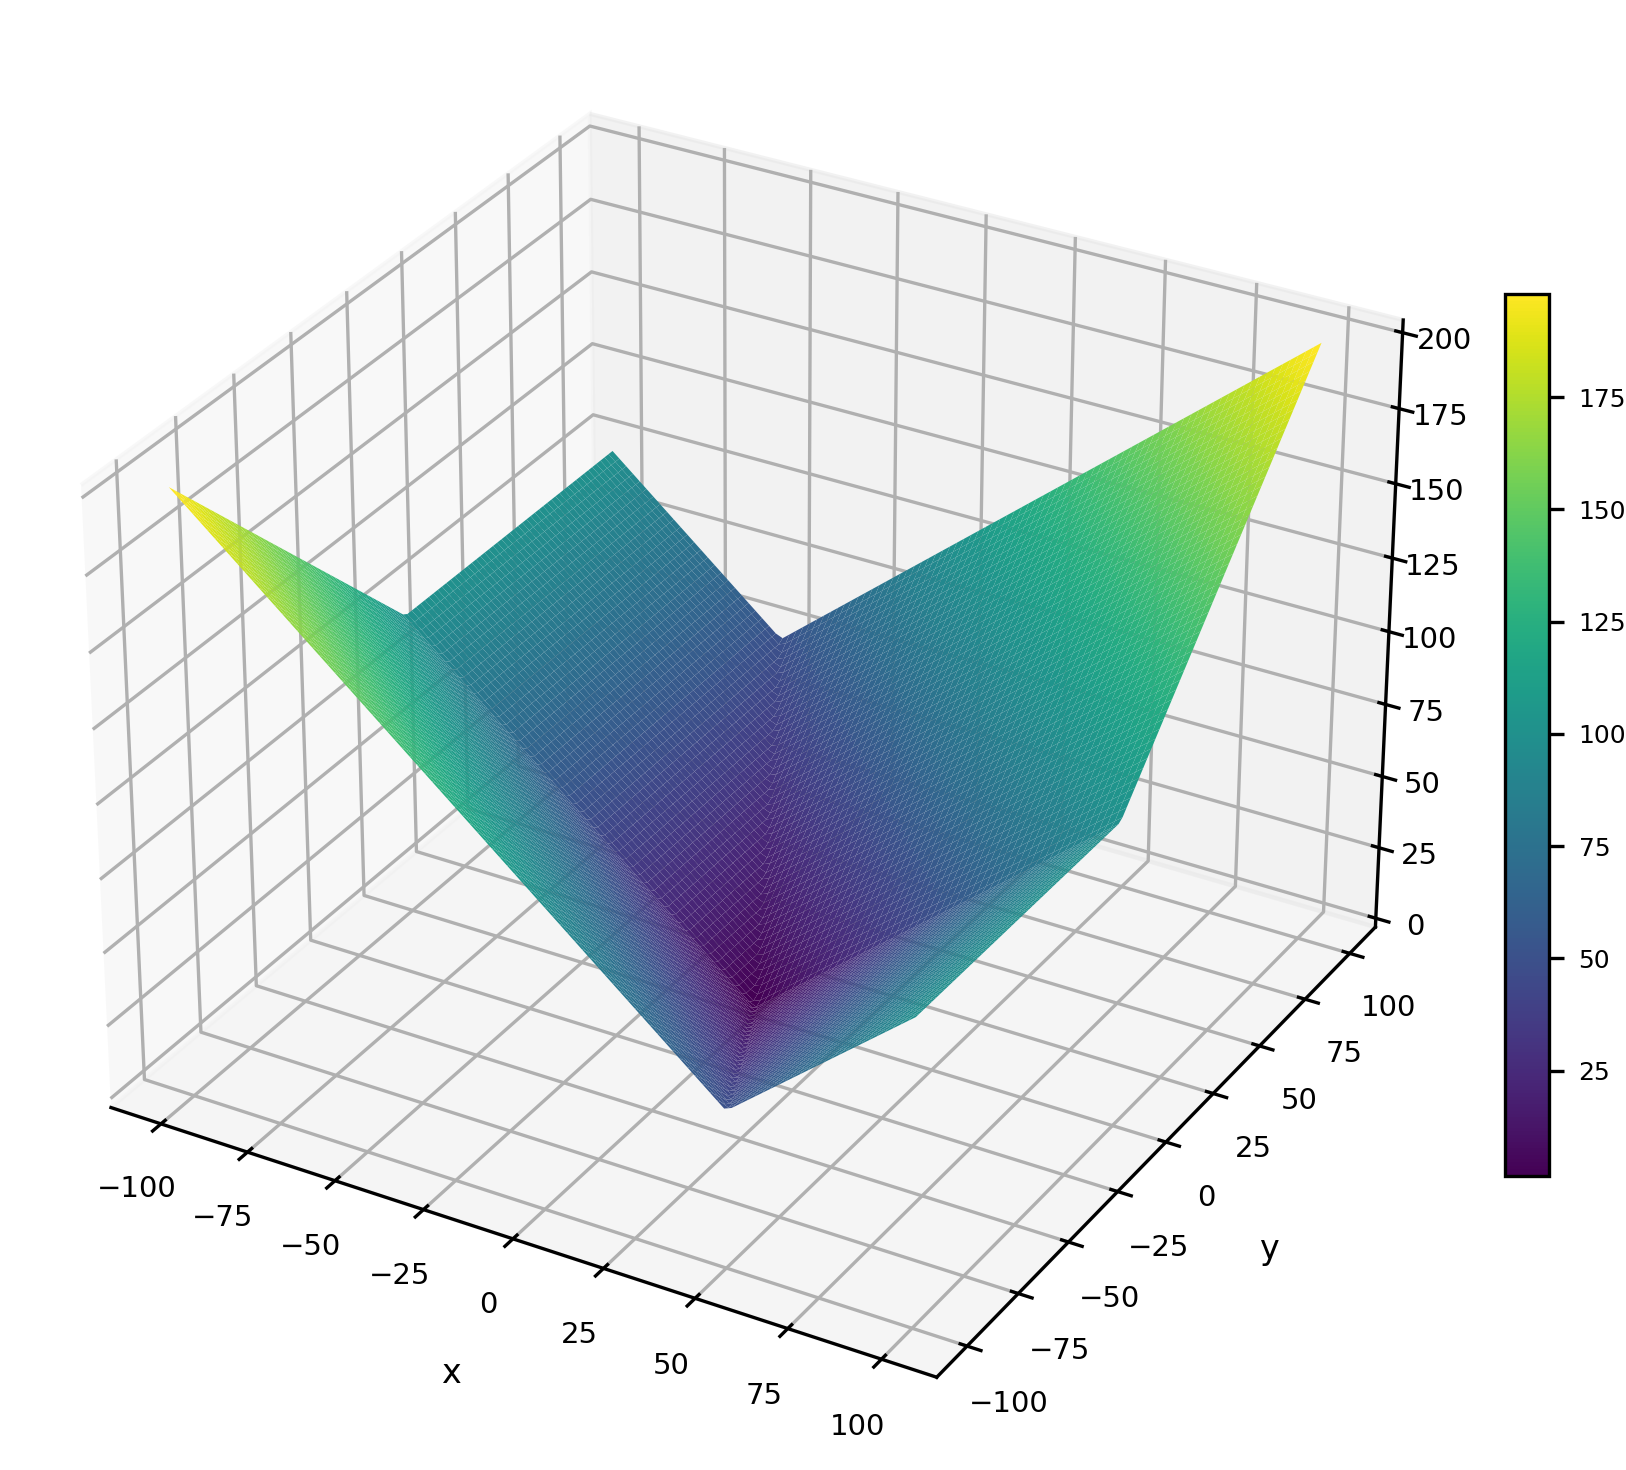
\includegraphics[width=1\textwidth]{Figures/benchmark_plots/Schwefel_N20_maximized.png}
        \caption{Schwefel N.2.0}
    \end{subfigure}
    % \hspace{.5cm} % Adjust the space as needed.
    \begin{subfigure}{0.32\textwidth}
        \centering
        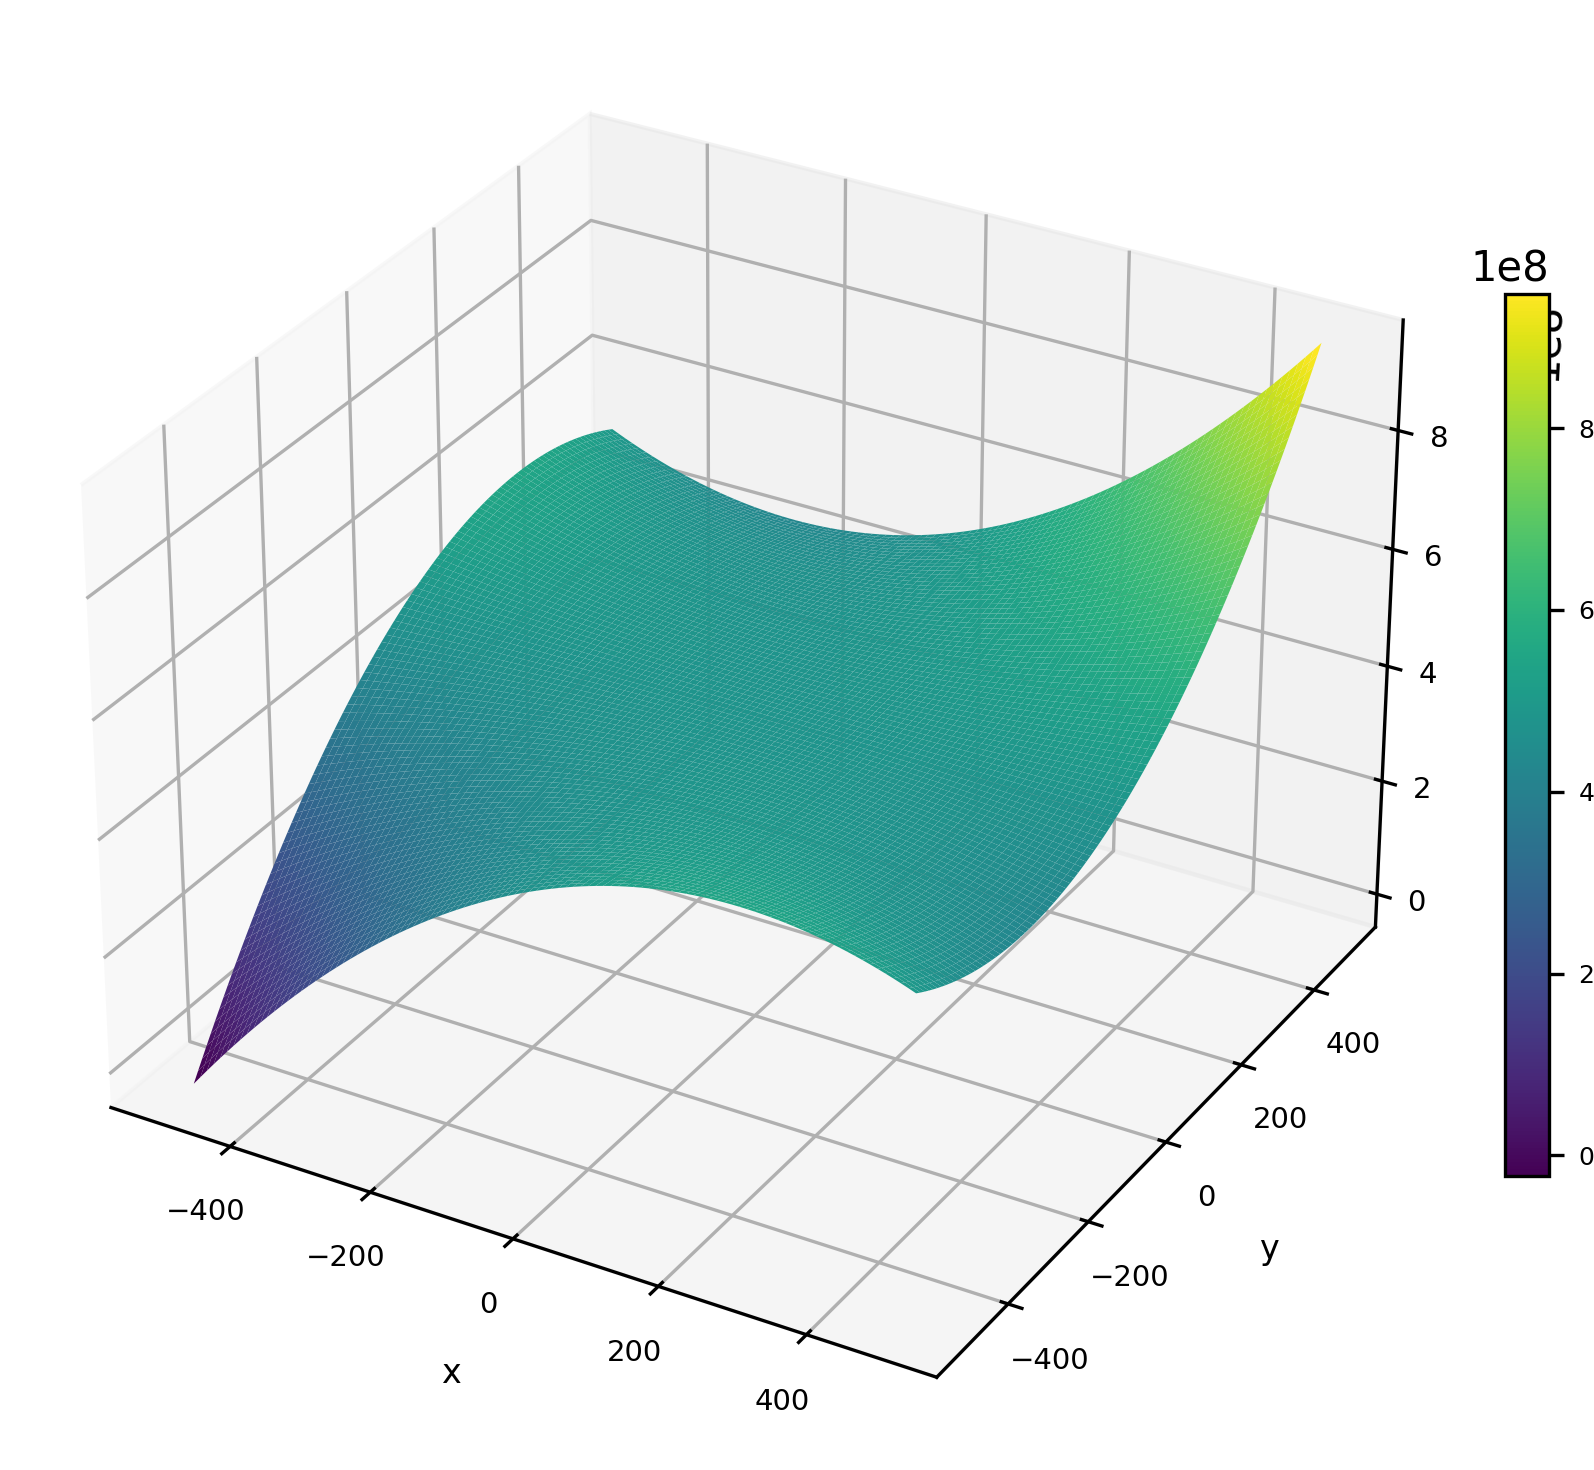
\includegraphics[width=1\textwidth]{Figures/benchmark_plots/Schwefel_N36_maximized.png}
        \caption{Schwefel N.3.6}
    \end{subfigure}
        \captionsetup{list=no}
\caption{Two-dimensional visualizations of benchmark problem landscapes.}
\end{figure}

\begin{figure}[p]\ContinuedFloat
\renewcommand\thesubfigure{A.\arabic{subfigure}} % Local change starts here
    \centering
    \begin{subfigure}{0.32\textwidth}
        \centering
        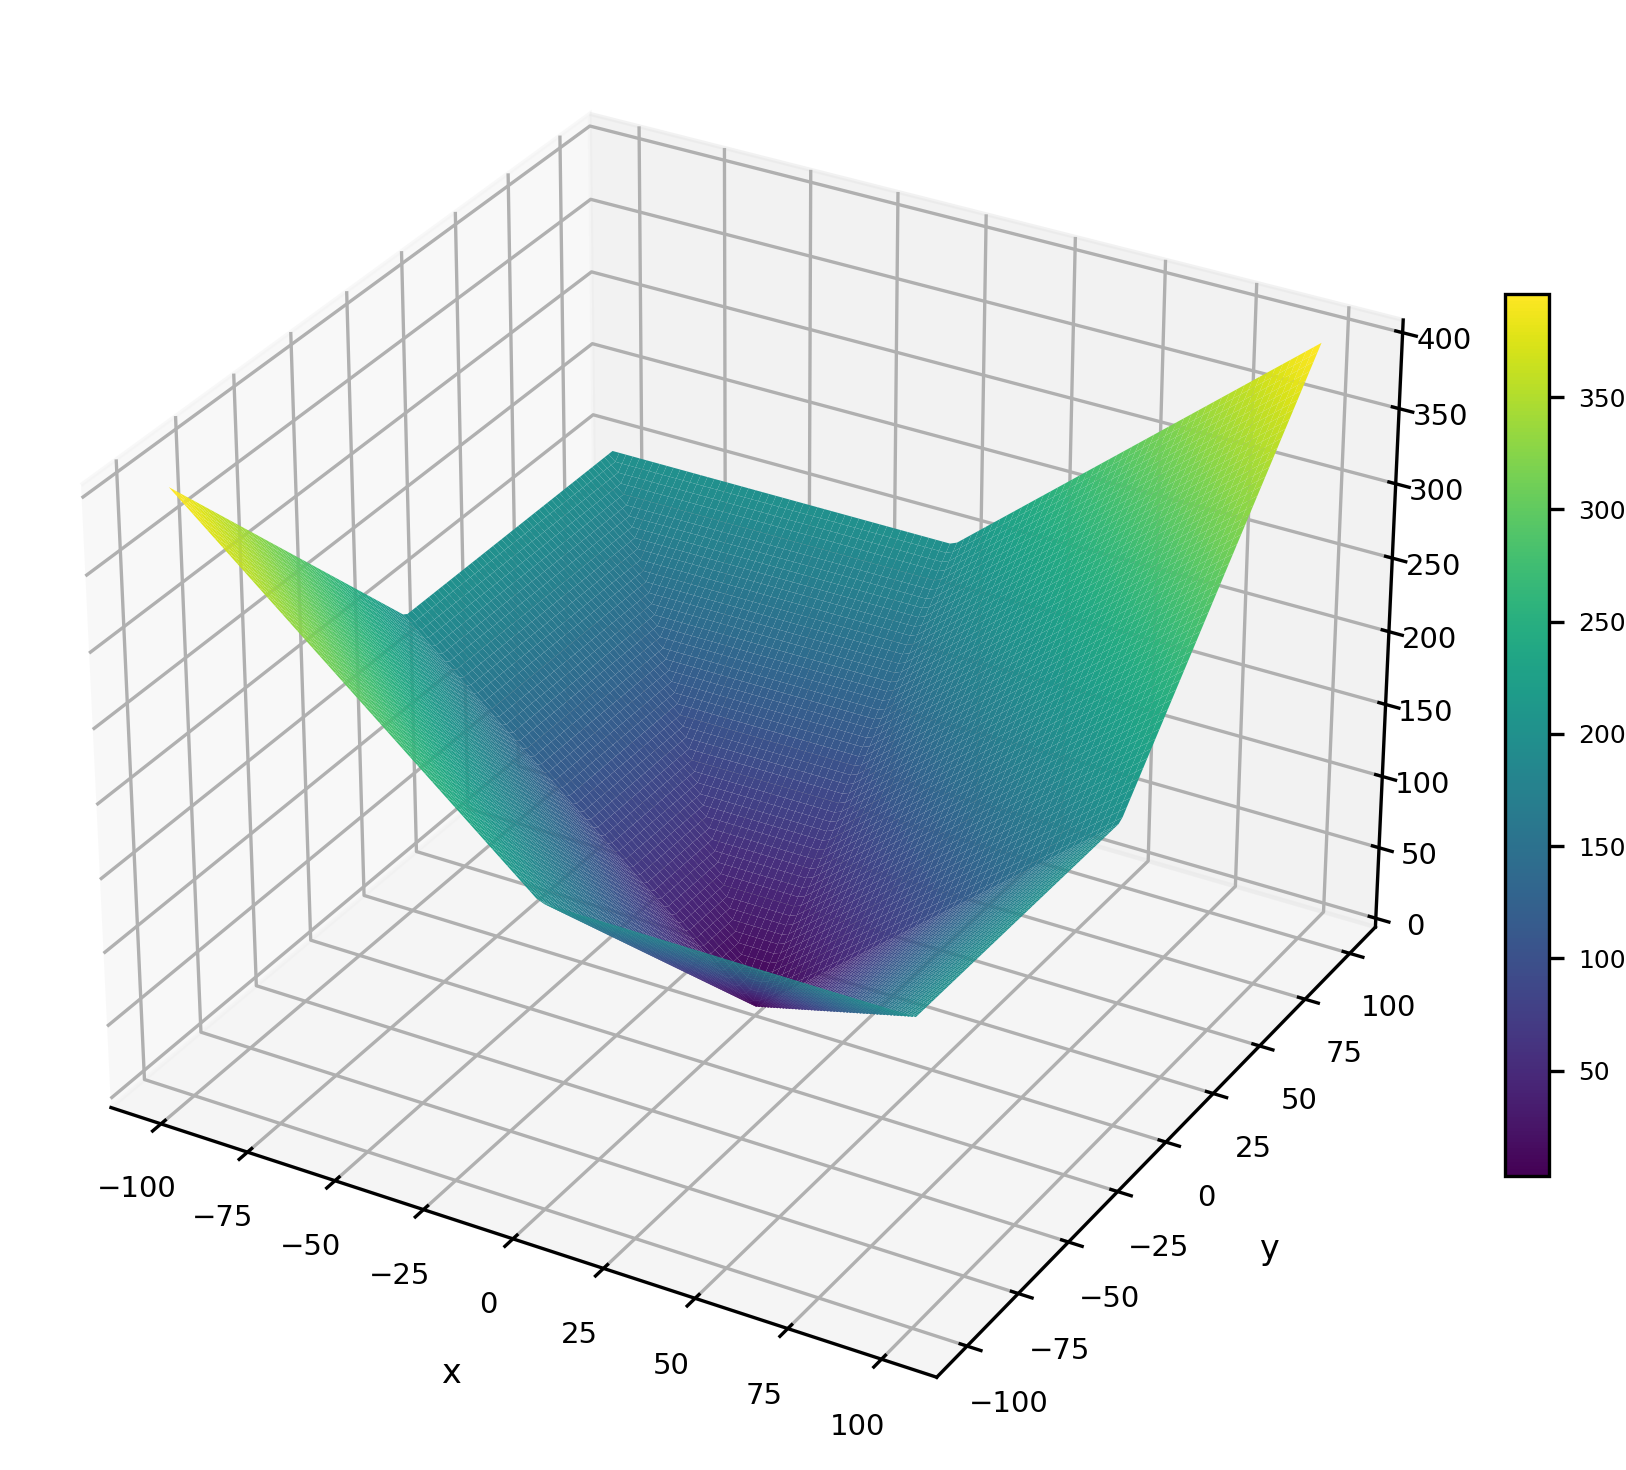
\includegraphics[width=1\textwidth]{Figures/benchmark_plots/Schwefel_N6_maximized.png}
        \caption{Schwefel N.6}
    \end{subfigure}
    % \hspace{.5cm} % Adjust the space as needed.
    \begin{subfigure}{0.32\textwidth}
        \centering
        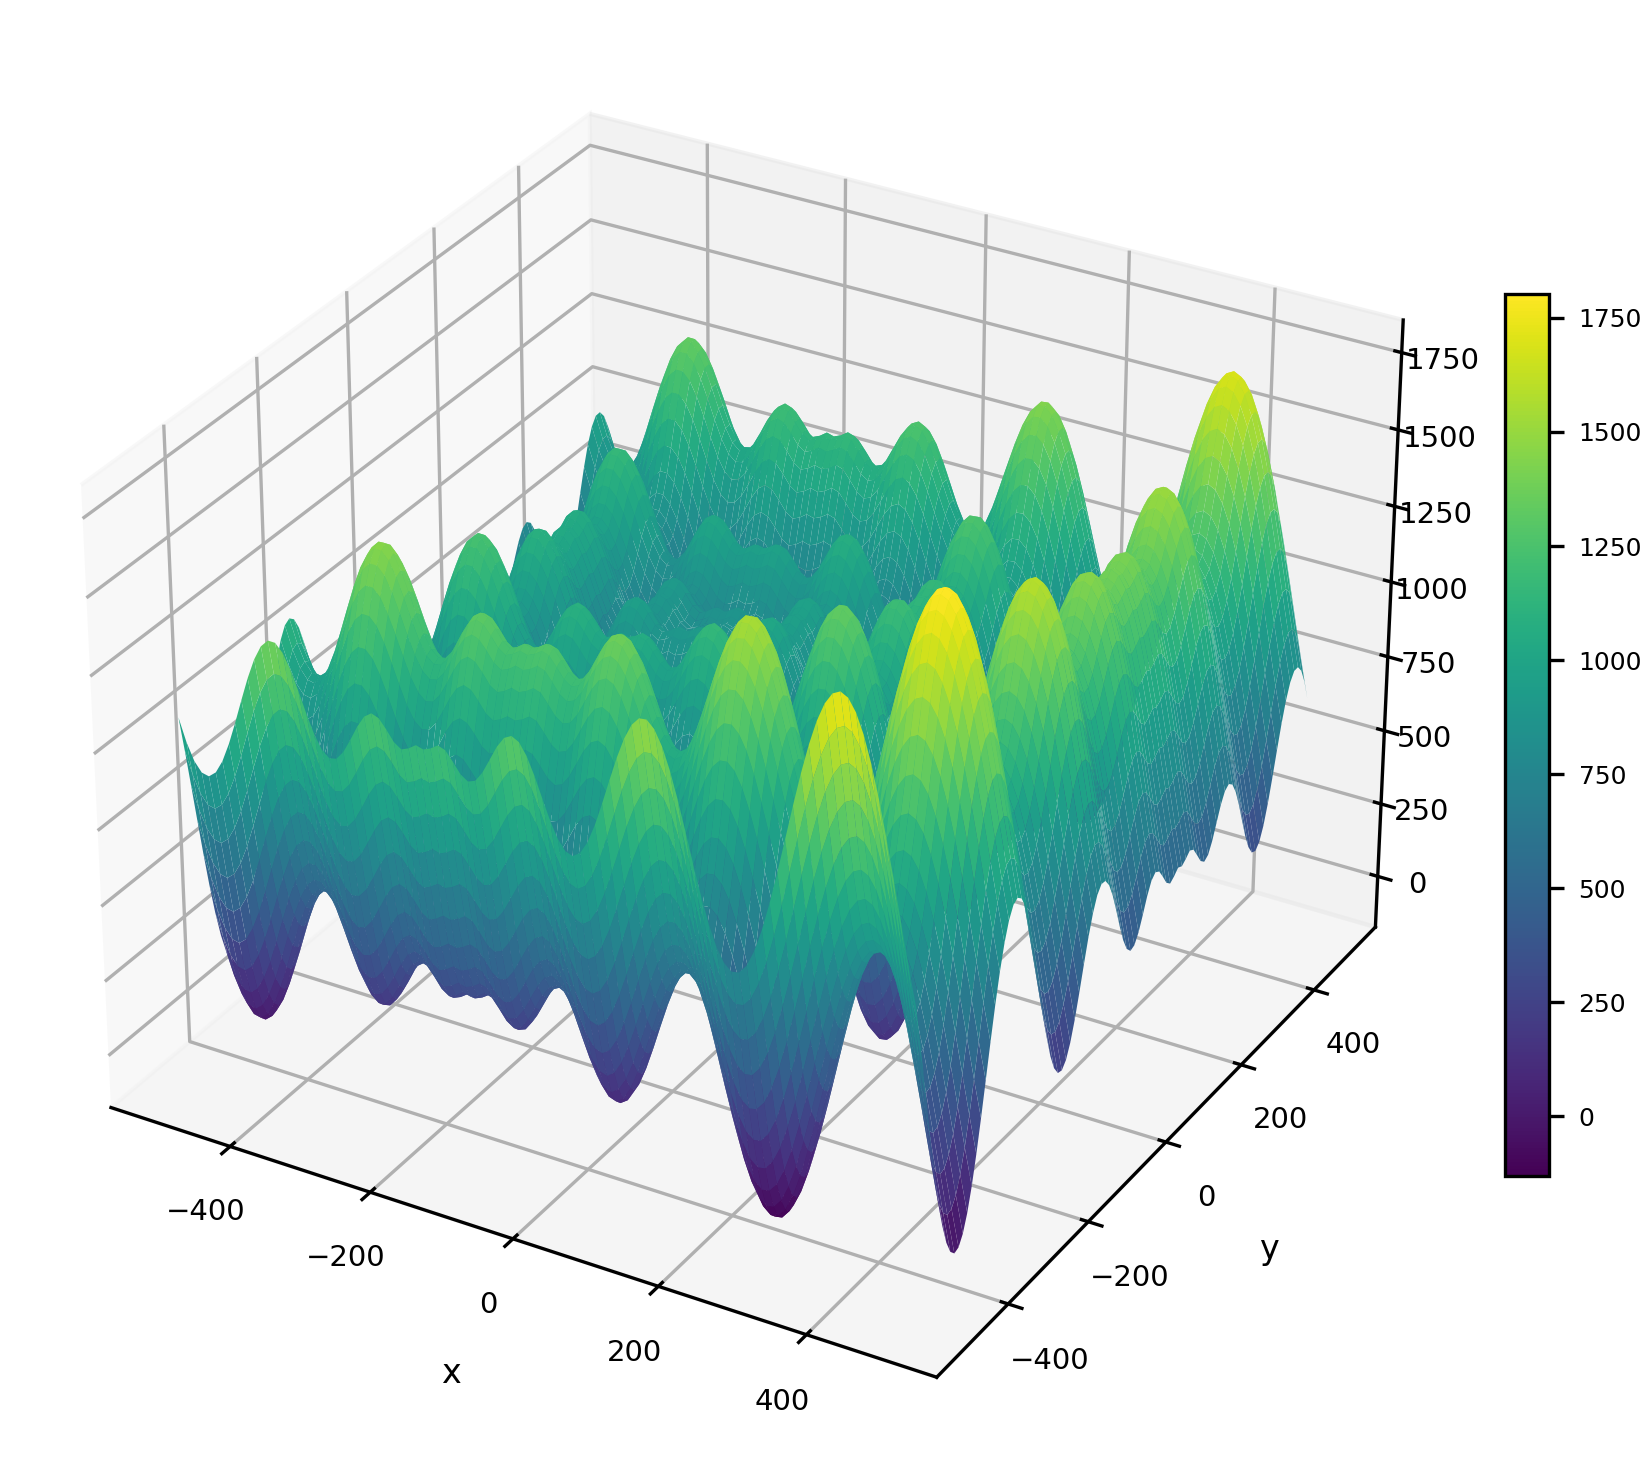
\includegraphics[width=1\textwidth]{Figures/benchmark_plots/Shifted_Schwefel_maximized.png}
        \caption{Shifted Schwefel (N.2.6)}
    \end{subfigure}
    \begin{subfigure}{0.32\textwidth}
        \centering
        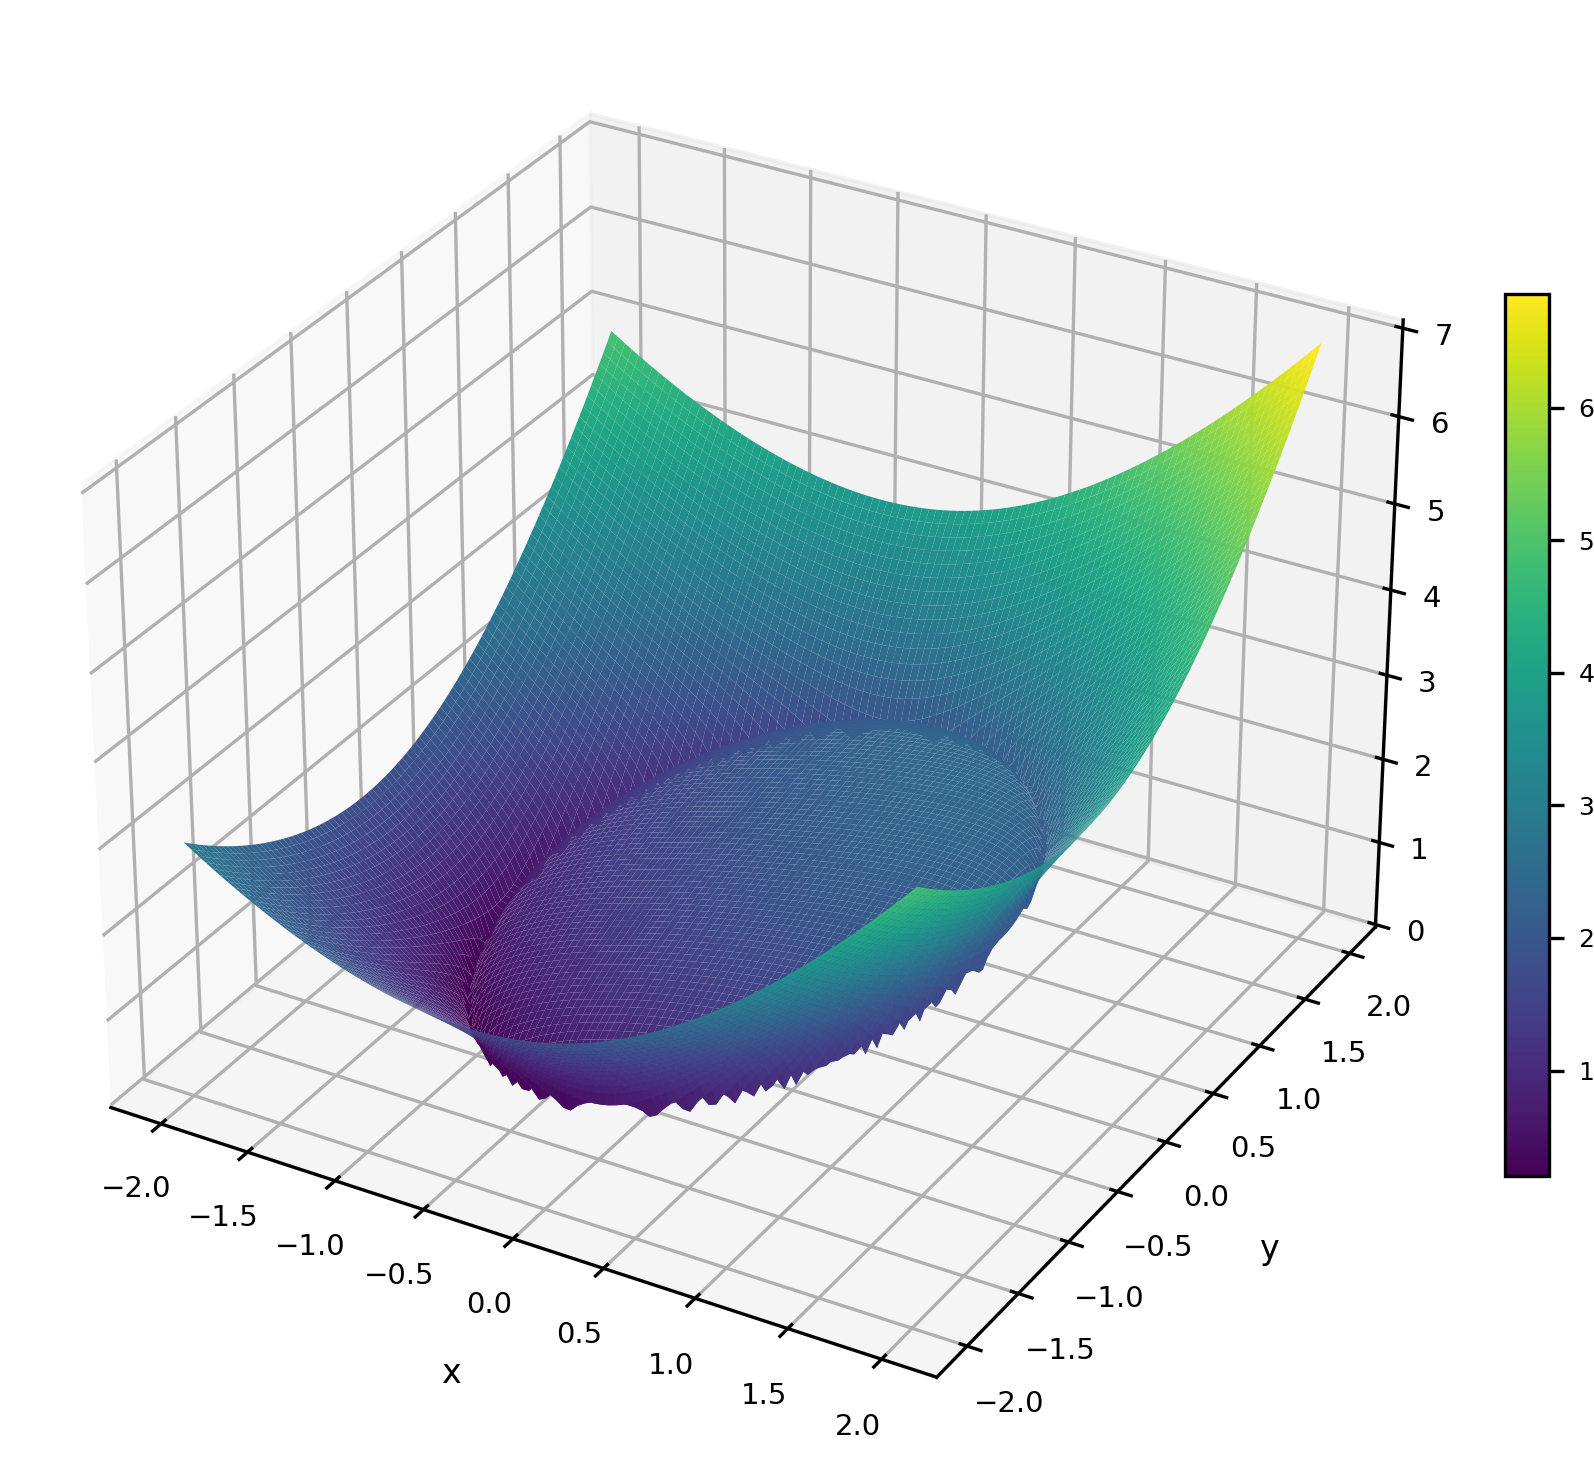
\includegraphics[width=1\textwidth]{Figures/benchmark_plots/Happy_Cat_maximized.png}
        \caption{HappyCat}
    \end{subfigure}
    % % \hspace{.5cm} % Adjust the space as needed.
    \begin{subfigure}{0.32\textwidth}
        \centering
        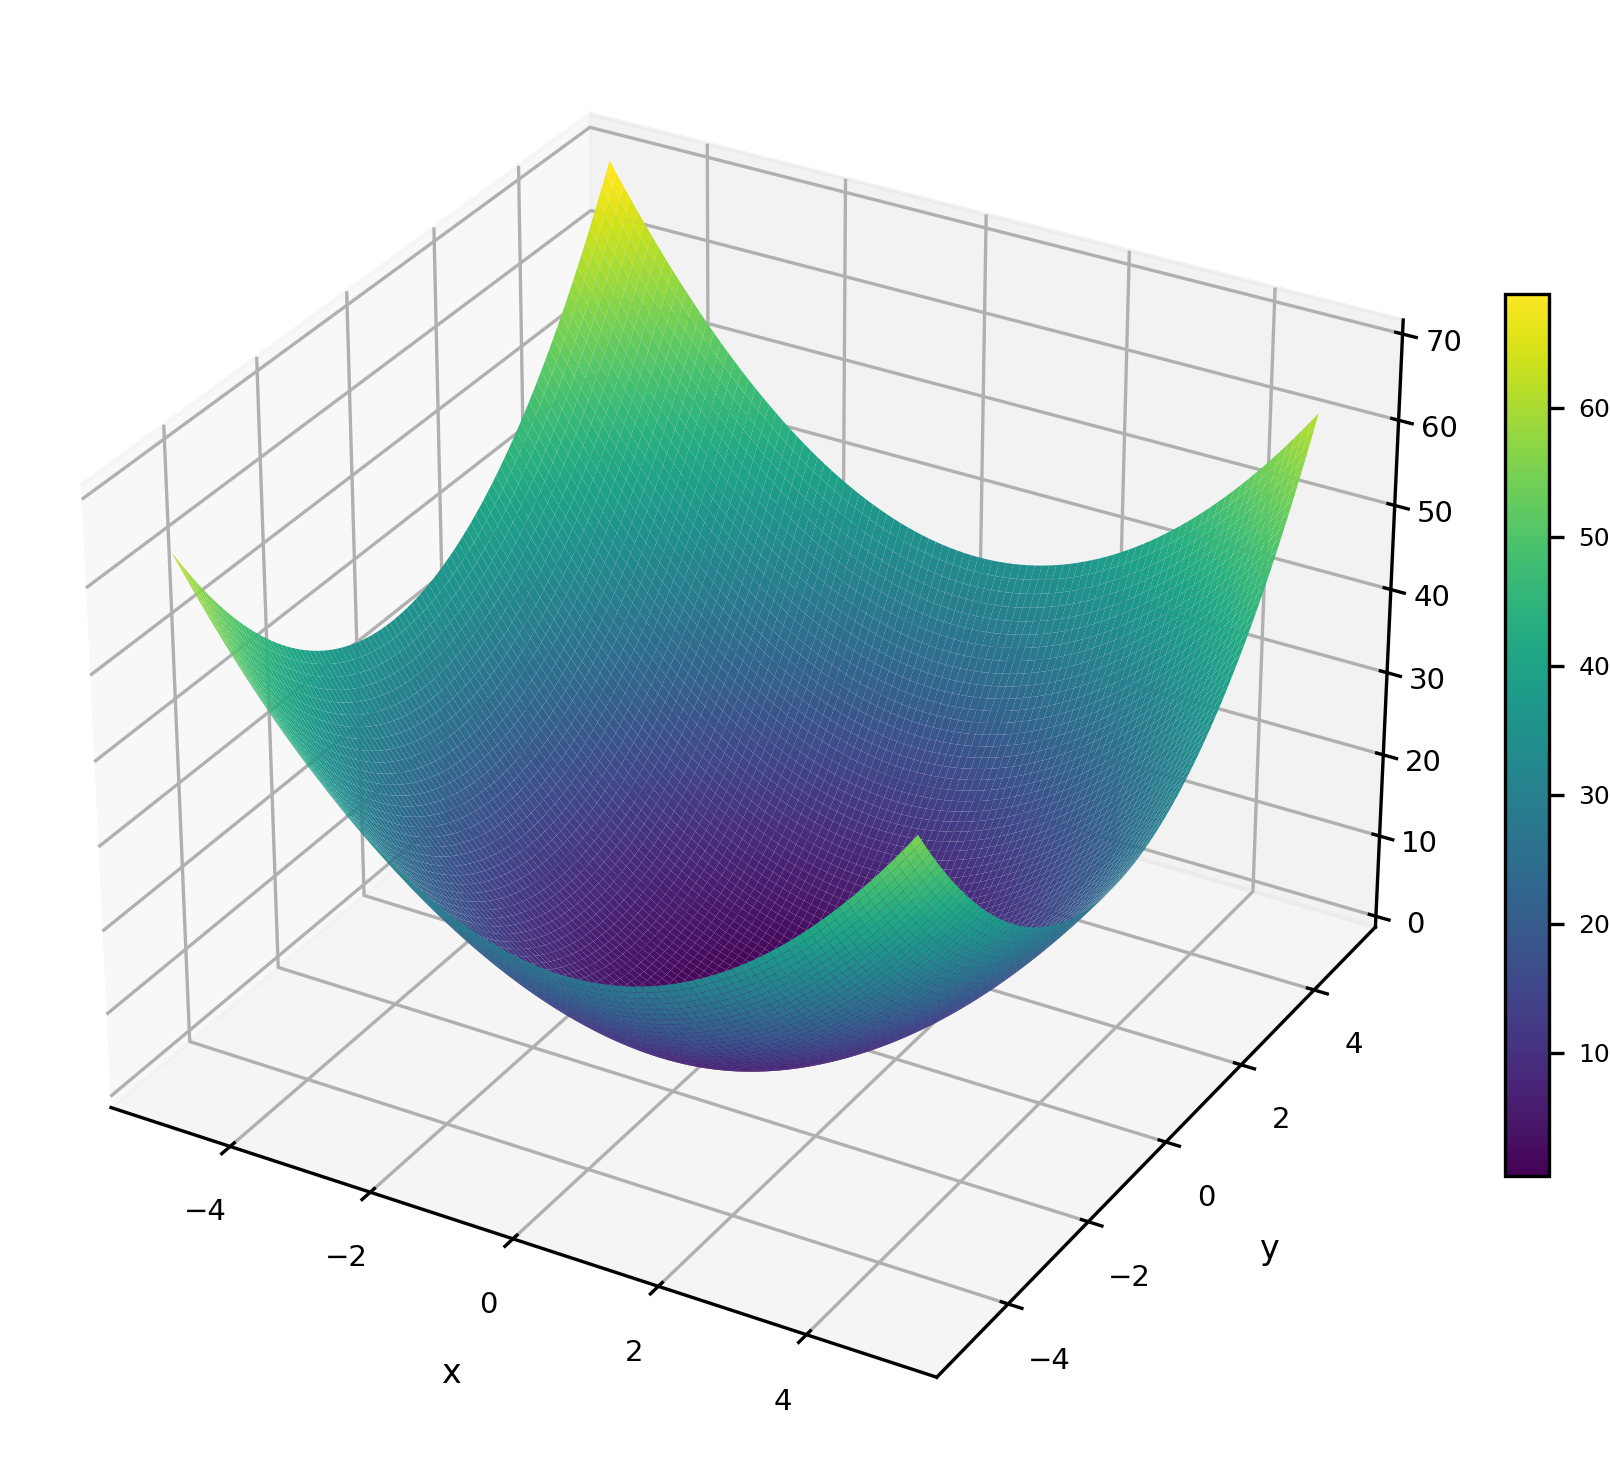
\includegraphics[width=1\textwidth]{Figures/benchmark_plots/Shifted_and_Rotated_HGBat_maximized.png}
        \caption{HGBat}
    \end{subfigure}
        \begin{subfigure}{0.32\textwidth}
        \centering
        \includegraphics[width=1\textwidth]{Figures/benchmark_plots/Shifted_and_Rotated_Expanded_Scaffer’s_F6_maximized.png}
        \caption{Schaffer F7}
    \end{subfigure}
        \begin{subfigure}{0.32\textwidth}
        \centering
        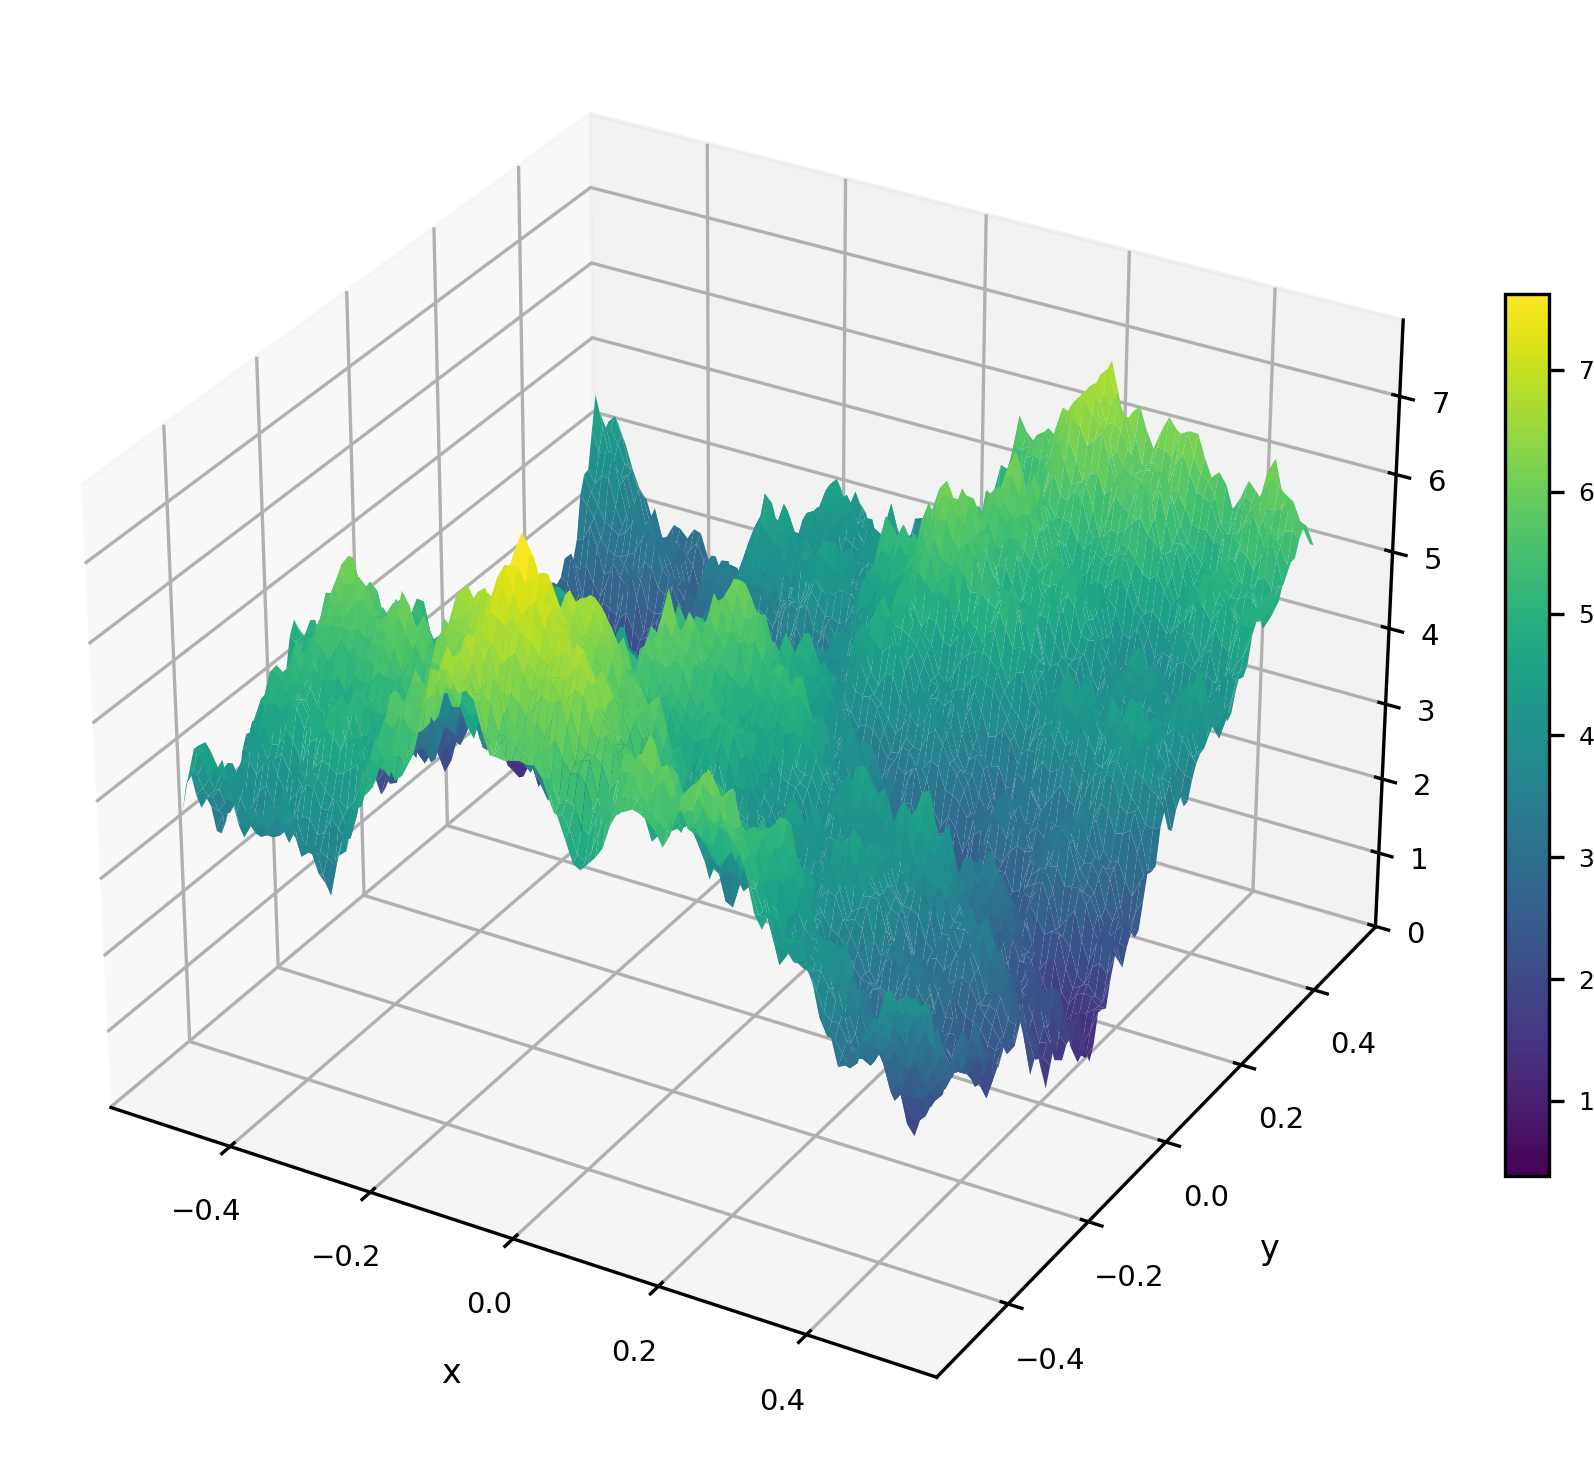
\includegraphics[width=1\textwidth]{Figures/benchmark_plots/Shifted_and_Rotated_Weierstrass_maximized.png}
        \caption{Weierstrass}
    \end{subfigure}
    % \hspace{.5cm} % Adjust the space as needed.
    \begin{subfigure}{0.32\textwidth}
        \centering
        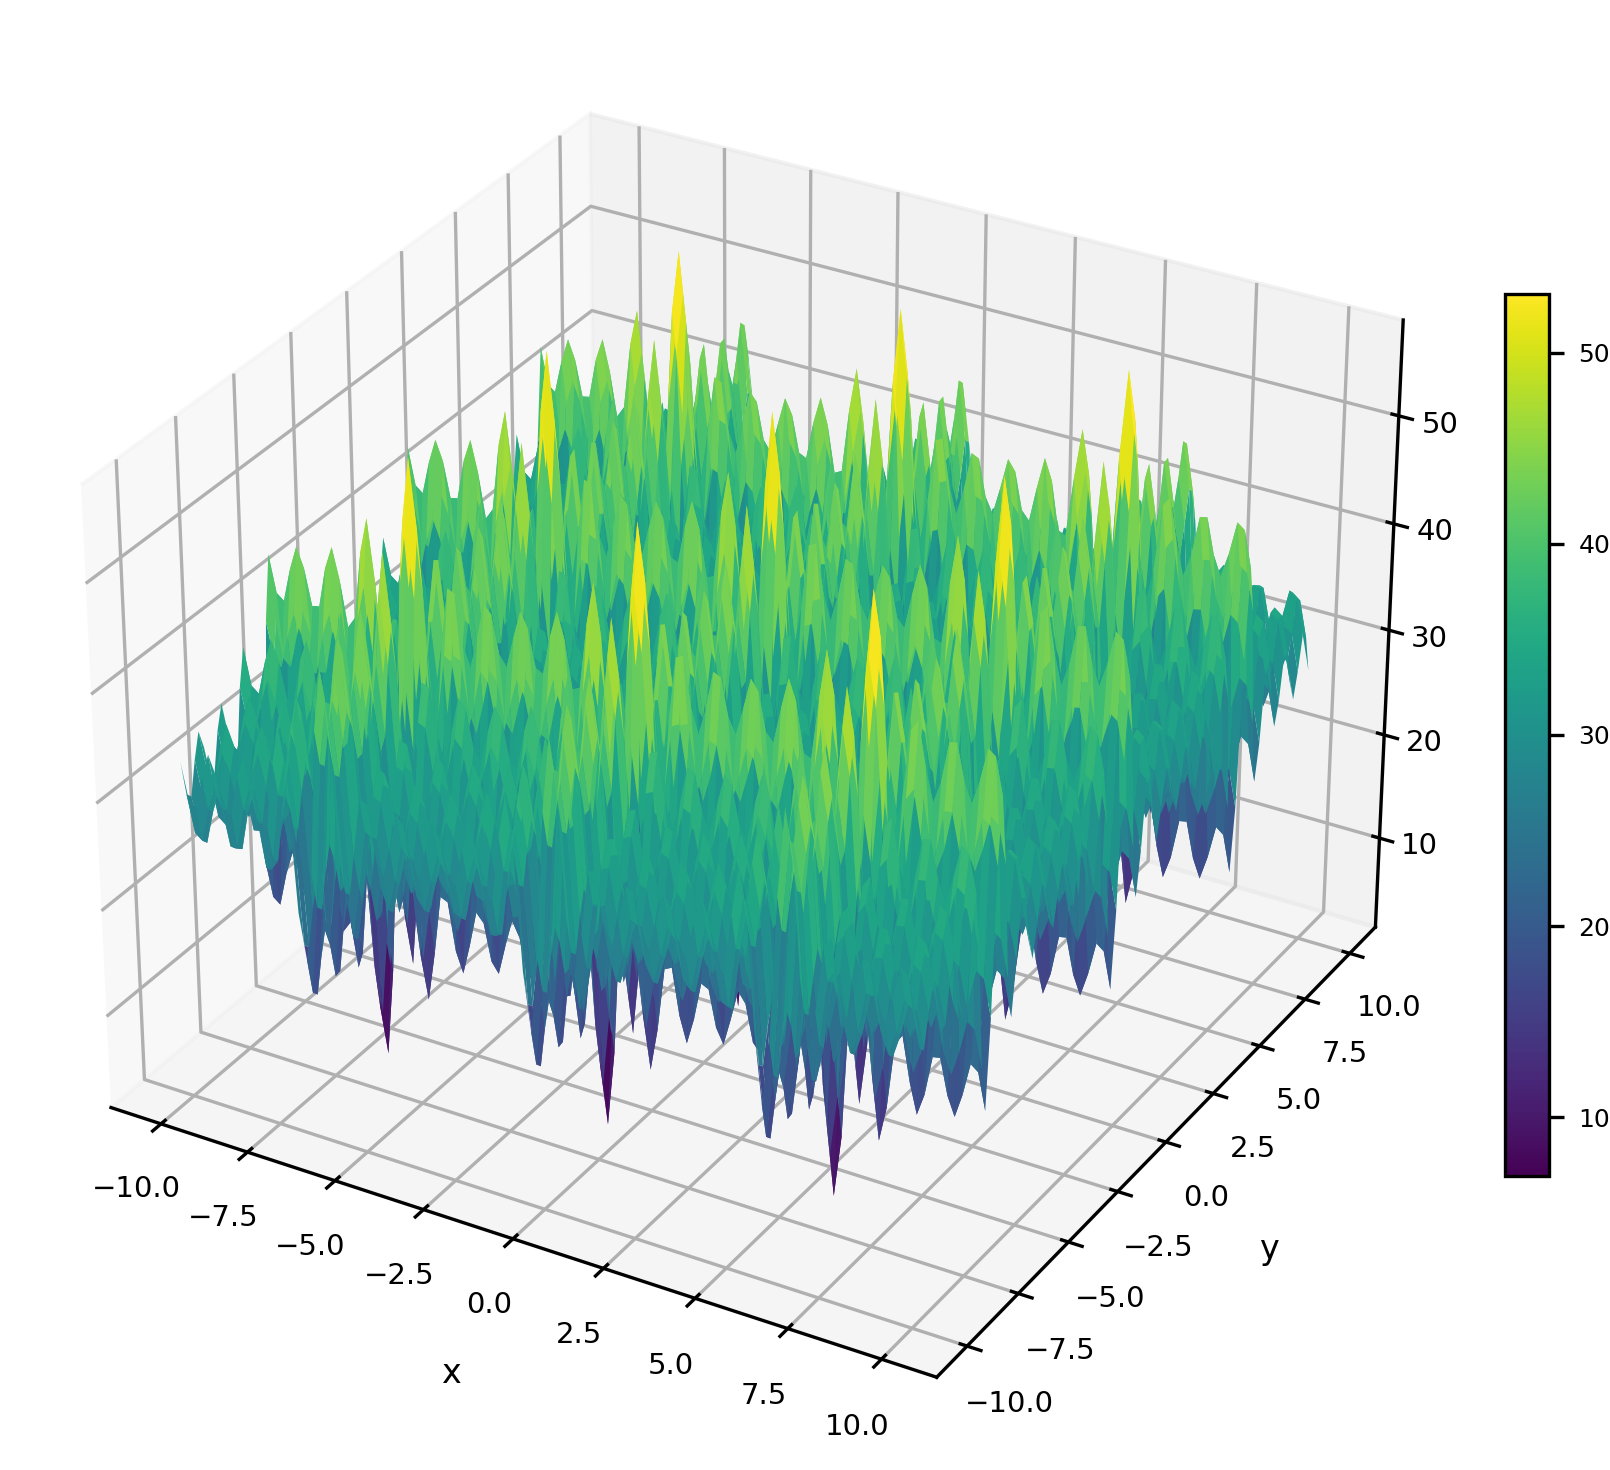
\includegraphics[width=1\textwidth]{Figures/benchmark_plots/Shubert_N3_maximized.png}
        \caption{Shubert N.3}
    \end{subfigure}
    % \hspace{.5cm} % Adjust the space as needed.
    \begin{subfigure}{0.32\textwidth}
        \centering
        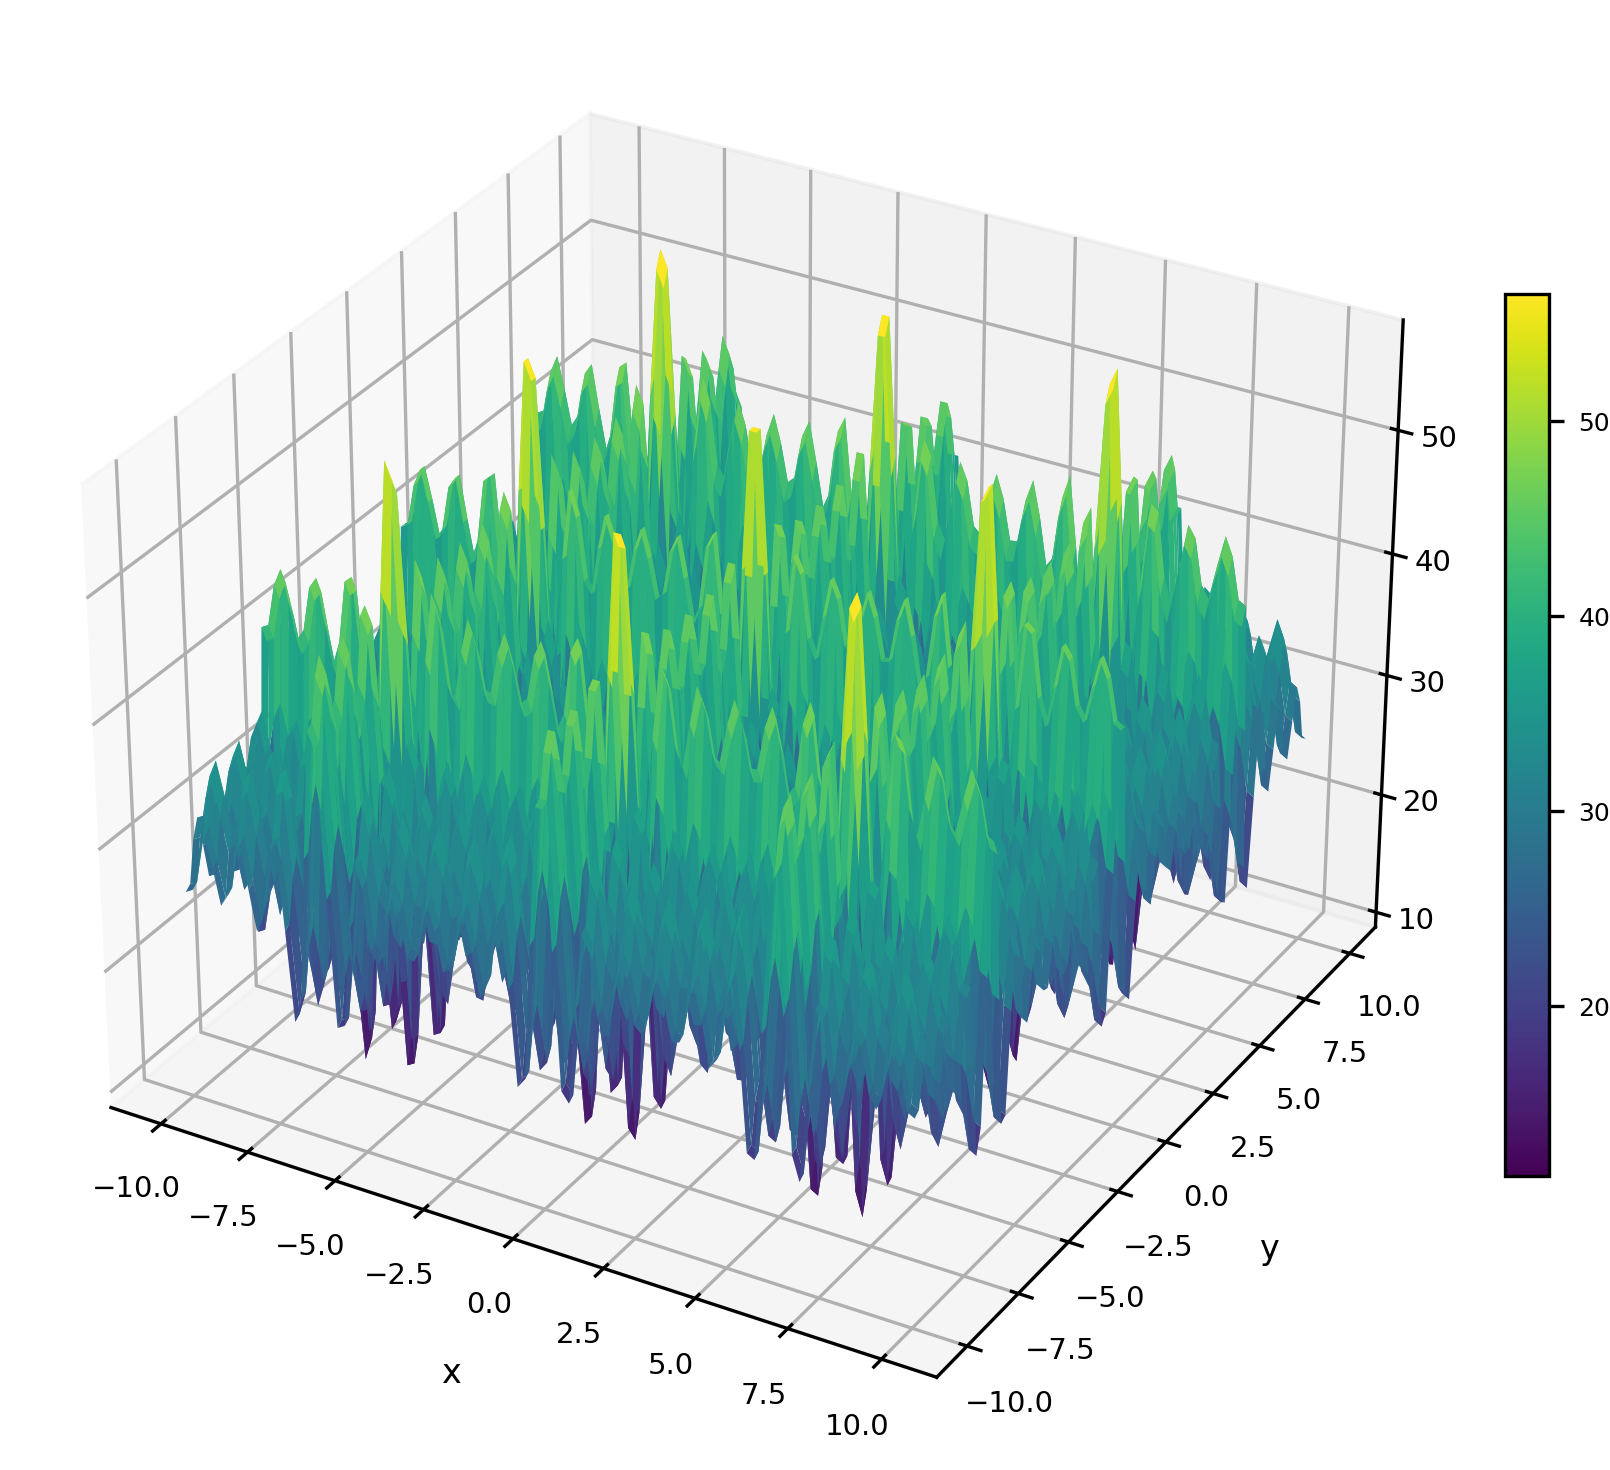
\includegraphics[width=1\textwidth]{Figures/benchmark_plots/Shubert_N4_maximized.png}
        \caption{Shubert N.4}
    \end{subfigure}
    % \hspace{.5cm} % Adjust the space as needed.
    \begin{subfigure}{0.32\textwidth}
        \centering
        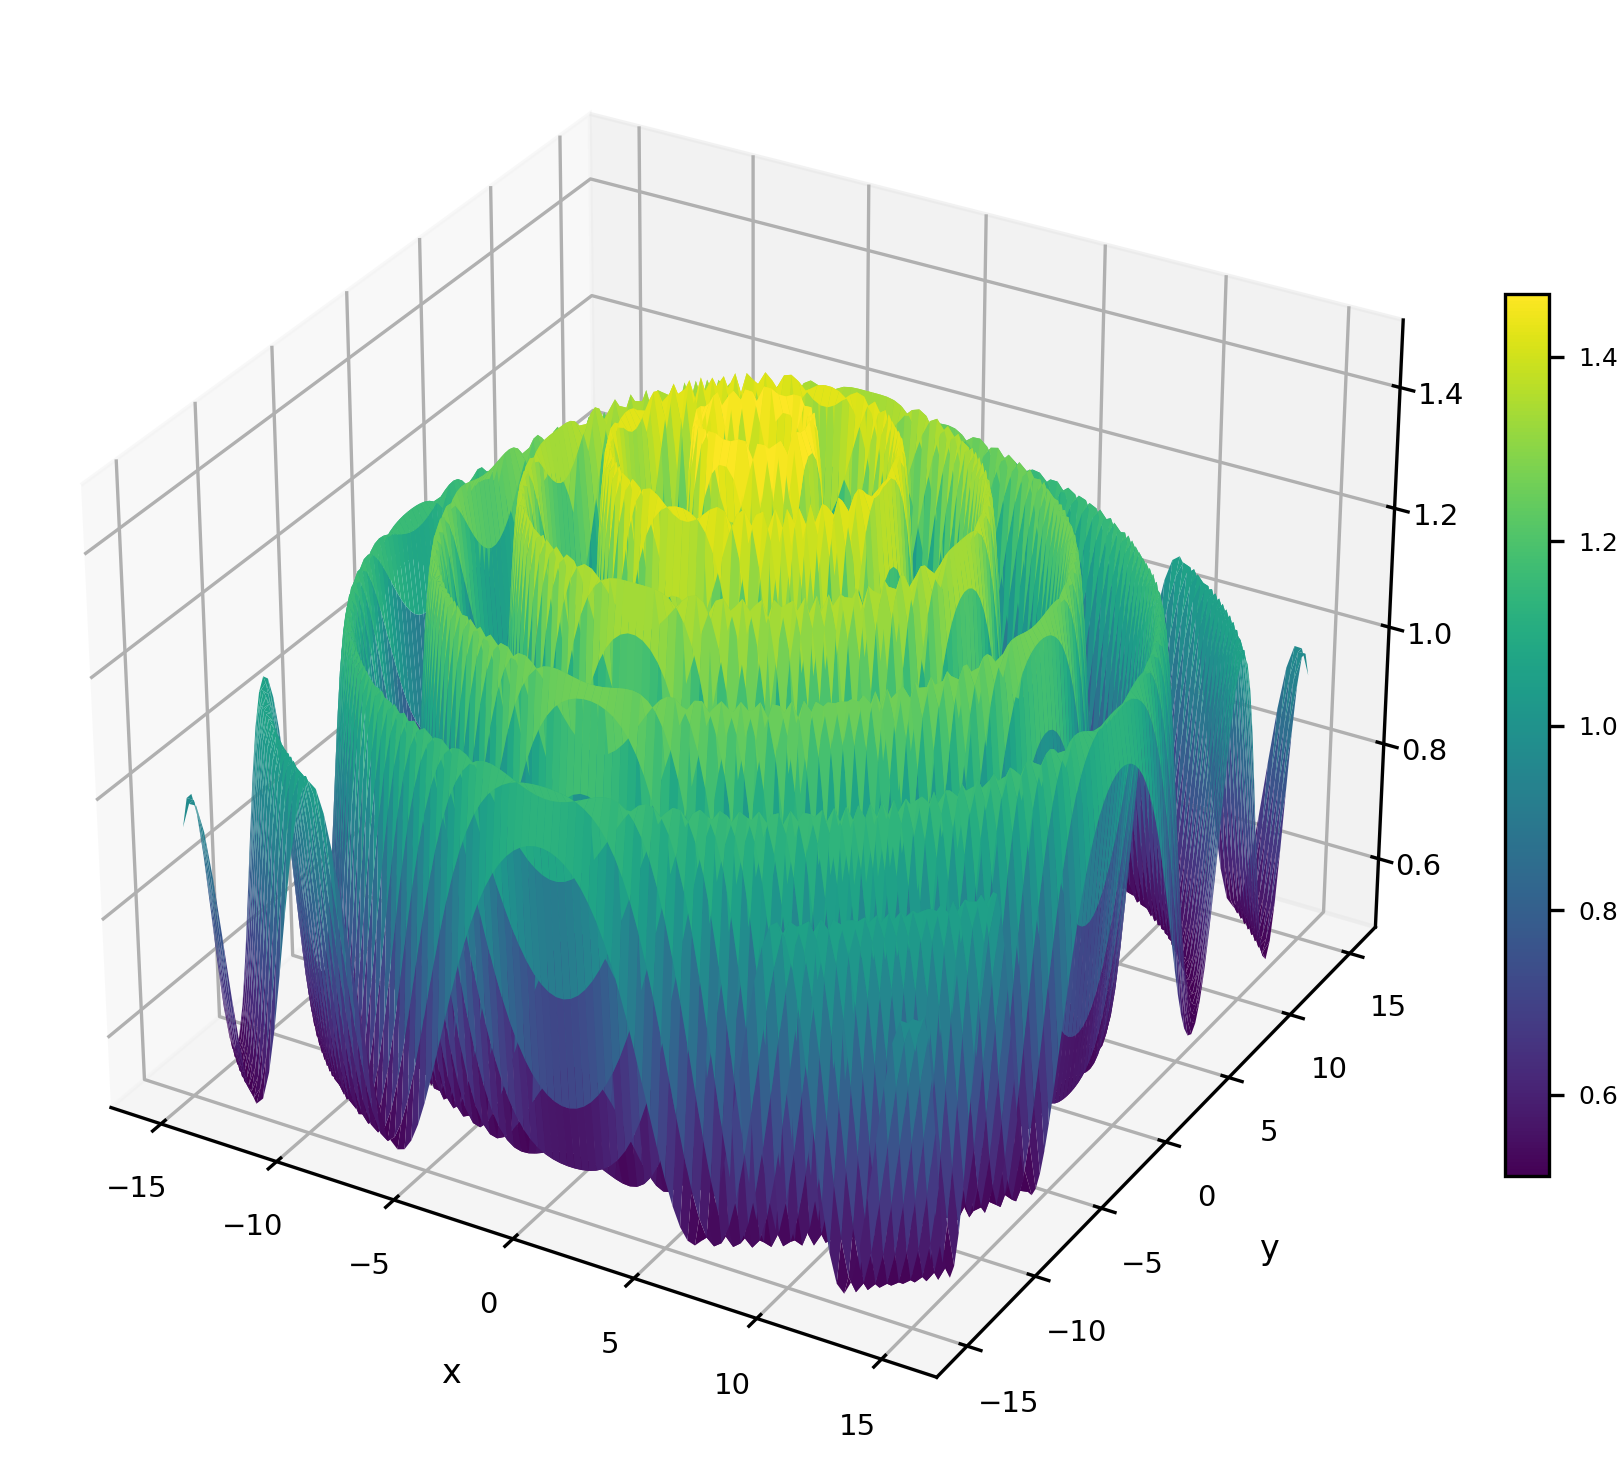
\includegraphics[width=1\textwidth]{Figures/benchmark_plots/SineEnvelope_maximized.png}
        \caption{Sine Envelope}
    \end{subfigure}
    \begin{subfigure}{0.32\textwidth}
        \centering
        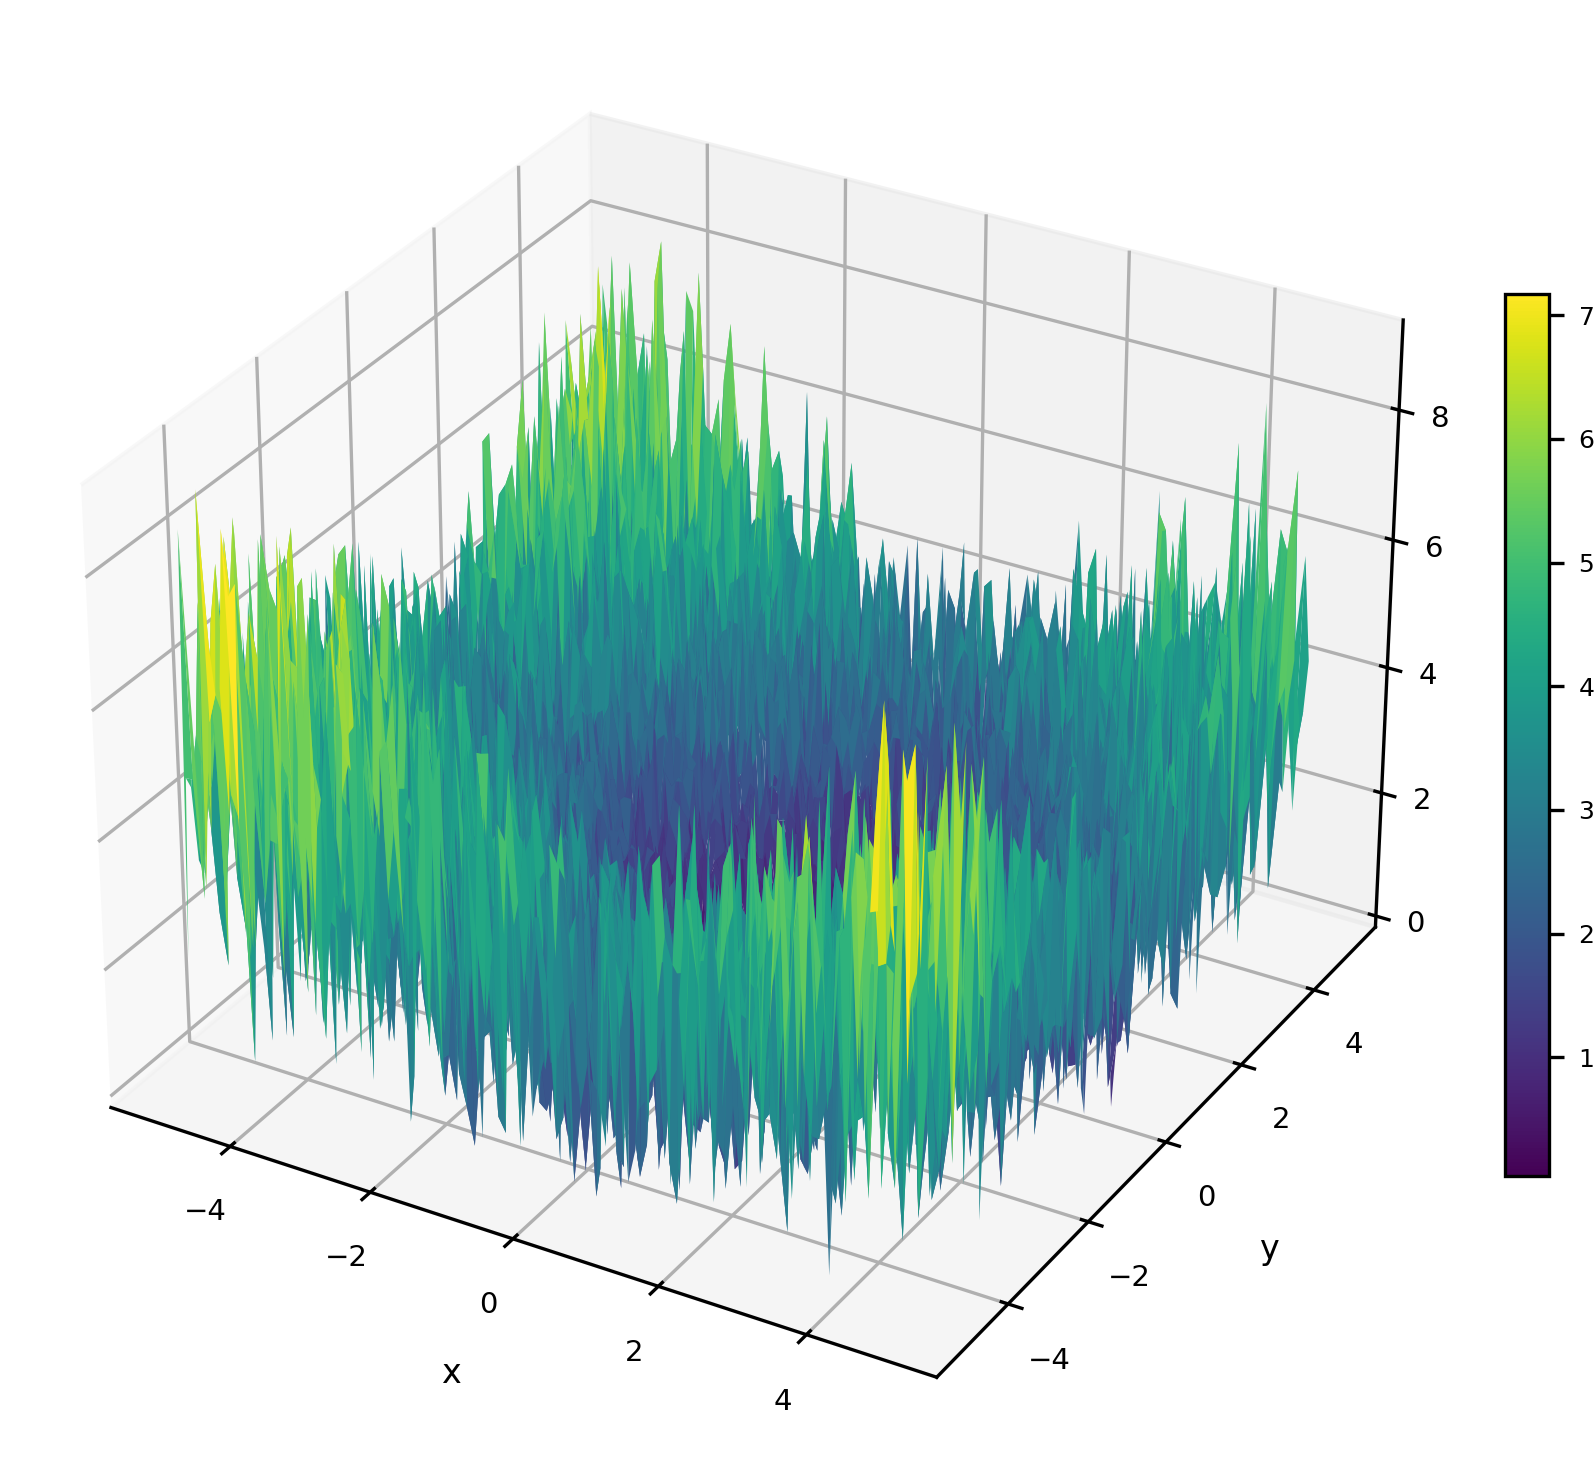
\includegraphics[width=1\textwidth]{Figures/benchmark_plots/Stochastic_maximized.png}
        \caption{Stochastic}
    \end{subfigure}
    % \hspace{.5cm} % Adjust the space as needed.
    \begin{subfigure}{0.32\textwidth}
        \centering
        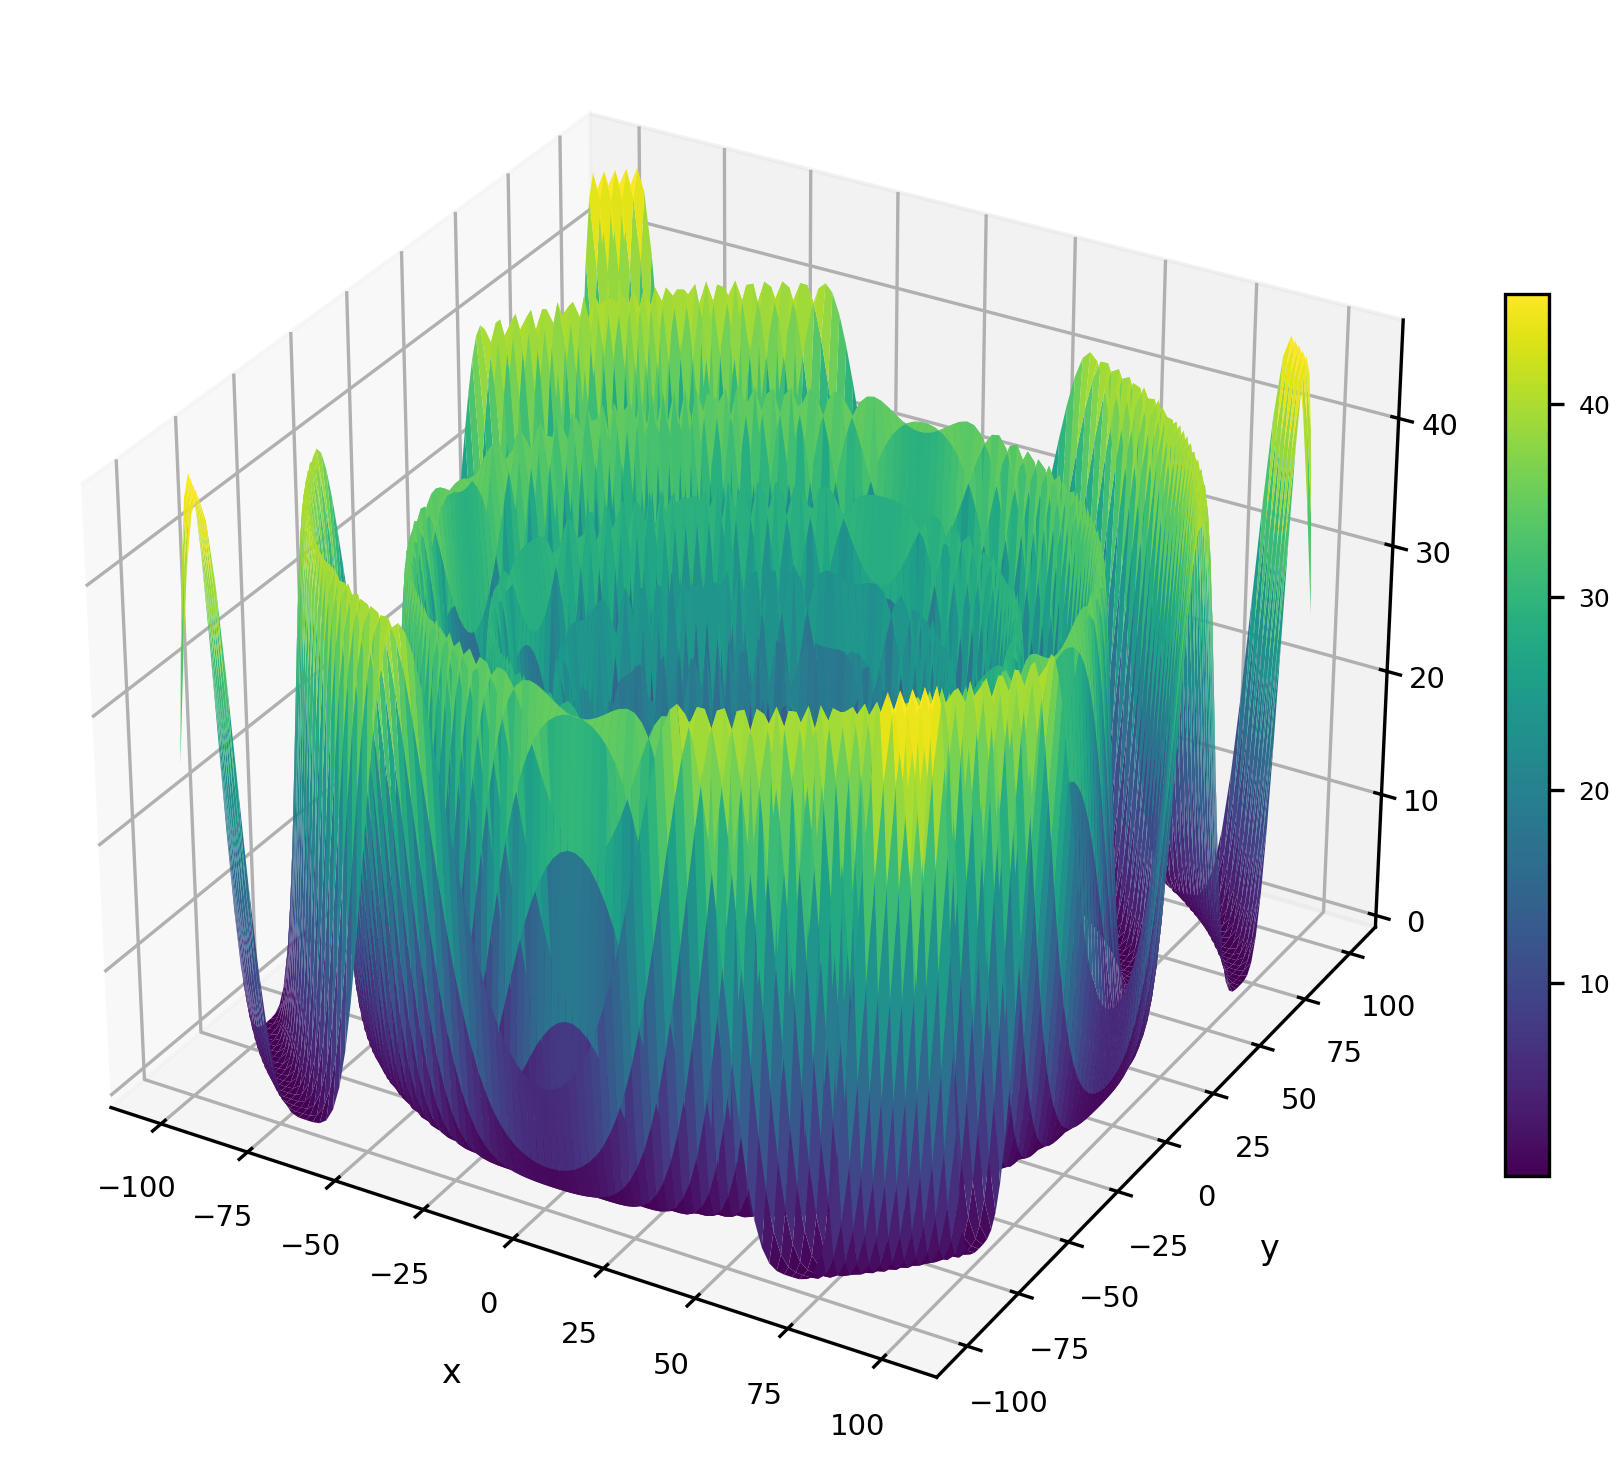
\includegraphics[width=1\textwidth]{Figures/benchmark_plots/StretchedV_maximized.png}
        \caption{Stretched V}
    \end{subfigure}
        \begin{subfigure}{0.32\textwidth}
        \centering
        \includegraphics[width=1\textwidth]{Figures/benchmark_plots/Styblinski–Tang_maximized.png}
        \caption{Styblinski–Tang}
    \end{subfigure}
        \captionsetup{list=no}
\caption{Two-dimensional visualizations of benchmark problem landscapes.}
\label{fig:benchmark_problems_plot}
\end{figure}
\chapter{Parameter Optimization Results}\label{app:optimization results}

\enlargethispage{1\baselineskip}
\begin{longtable}{l
*{15}{>{\centering\arraybackslash}p{0.6cm}}
}
\caption[Parameter configurations]{Algorithm parameter configurations used in the experiments.}
\label{tab:parameter_configuration}\\
\toprule
\adjustbox{angle=90}{\textbf{Parameter}} &
\adjustbox{angle=90}{\textbf{PSO}} &
\adjustbox{angle=90}{\textbf{PerturbationPSO}} &
\adjustbox{angle=90}{\textbf{RebelPSO}} &
\adjustbox{angle=90}{\textbf{RejectorPSO}} &
\adjustbox{angle=90}{\textbf{RebelRejectorPSO}} &
\adjustbox{angle=90}{\textbf{ContrarianPSO}} &
\adjustbox{angle=90}{\textbf{DefeatistPSO}} &
\adjustbox{angle=90}{\textbf{ContrarianDefeatistPSO}} &
\adjustbox{angle=90}{\textbf{EschewerPSO}} &
\adjustbox{angle=90}{\textbf{EscapistPSO}} &
\adjustbox{angle=90}{\textbf{EschewerEscapistPSO}} &
\adjustbox{angle=90}{\textbf{HybridFullDisjointPSO}} &
\adjustbox{angle=90}{\textbf{HybridPartialDisjointPSO}} &
\adjustbox{angle=90}{\textbf{HybridAdditivePSO}} \\
\midrule
\endfirsthead

\toprule
\adjustbox{angle=90}{\textbf{Parameter}} &
\adjustbox{angle=90}{\textbf{PSO}} &
\adjustbox{angle=90}{\textbf{PerturbationPSO}} &
\adjustbox{angle=90}{\textbf{RebelPSO}} &
\adjustbox{angle=90}{\textbf{RejectorPSO}} &
\adjustbox{angle=90}{\textbf{RebelRejectorPSO}} &
\adjustbox{angle=90}{\textbf{ContrarianPSO}} &
\adjustbox{angle=90}{\textbf{DefeatistPSO}} &
\adjustbox{angle=90}{\textbf{ContrarianDefeatistPSO}} &
\adjustbox{angle=90}{\textbf{EschewerPSO}} &
\adjustbox{angle=90}{\textbf{EscapistPSO}} &
\adjustbox{angle=90}{\textbf{EschewerEscapistPSO}} &
\adjustbox{angle=90}{\textbf{HybridFullDisjointPSO}} &
\adjustbox{angle=90}{\textbf{HybridPartialDisjointPSO}} &
\adjustbox{angle=90}{\textbf{HybridAdditivePSO}} \\
\midrule
\endhead
$N$   & 100 & 100 & 100 & 100 & 100 & 100 & 100 & 100 & 100 & 100 & 100 & 100 & 100 & 100 \\
$\omega$   & 0.063 & 0.637 & 0.131 & 0.084 & 0.116 & 0.102 & 0.069 & 0.067 & 0.091 & 0.047 & 0.088 & 0.010 & 0.054 & 0.043 \\
$c_1$      & 4.373 & 2.545 & 0.308 & 1.545 & 1.292 & 0.405 & 0.405 & 0.905 & 2.177 & 2.577 & 0.900 & 2.519 & 5.251 & 0.254 \\
$c_2$      & 2.755 & 0.789 & 5.531 & 5.918 & 4.833 & 5.729 & 5.296 & 5.063 & 3.649 & 5.865 & 5.271 & 1.959 & 1.044 & 2.307 \\
$c_3$      & --    & --    & 3.923 & --    & 3.745 & --    & --    & --    & --    & --    & --    & 1.523 & 0.445 & 0.041 \\
$c_4$      & --    & --    & --    & 0.466 & 1.441 & --    & --    & --    & --    & --    & --    & 0.805 & 0.108 & 1.304 \\
$c_5$      & --    & --    & --    & --    & --    & 4.560 & --    & 4.333 & --    & --    & --    & 4.525 & 0.792 & 2.243 \\
$c_6$      & --    & --    & --    & --    & --    & --    & 0.953 & 1.746 & --    & --    & --    & 0.353 & 0.068 & 0.137 \\
$c_7$      & --    & --    & --    & --    & --    & --    & --    & --    & 1.658 & --    & 4.853 & 3.545 & 3.732 & 2.769 \\
$c_8$      & --    & --    & --    & --    & --    & --    & --    & --    & --    & 0.059 & 1.582 & 2.257 & 5.558 & 0.023 \\
$\sigma$   & --    & 0.008 & --    & --    & --    & --    & --    & --    & --    & --    & --    & --    & --    & --    \\
$\rho_1$   & --    & --    & --    & --    & --    & --    & --    & --    & --    & --    & --    & --    & --    & 0.880 \\
$\rho_2$   & --    & --    & --    & --    & --    & --    & --    & --    & --    & --    & --    & --    & --    & 0.764 \\
$\rho_3$   & --    & --    & 0.180 & --    & 0.189 & --    & --    & --    & --    & --    & --    & 0.071 & 0.114 & 0.476 \\
$\rho_4$   & --    & --    & --    & 0.679 & 0.194 & --    & --    & --    & --    & --    & --    & 0.353 & 0.393 & 0.536 \\
$\rho_5$   & --    & --    & --    & --    & --    & 0.480 & --    & 0.122 & --    & --    & --    & 0.035 & 0.365 & 0.460 \\
$\rho_6$   & --    & --    & --    & --    & --    & --    & 0.528 & 0.192 & --    & --    & --    & 0.388 & 0.570 & 0.539 \\
$\rho_7$   & --    & --    & --    & --    & --    & --    & --    & --    & 0.224 & --    & 0.163 & 0.136 & 0.172 & 0.315 \\
$\rho_8$   & --    & --    & --    & --    & --    & --    & --    & --    & --    & 0.476 & 0.230 & 0.016 & 0.038 & 0.463 \\
\bottomrule
\end{longtable}


\begin{figure}[H]
    \centering
    \begin{subfigure}{0.49\textwidth}
        \centering
        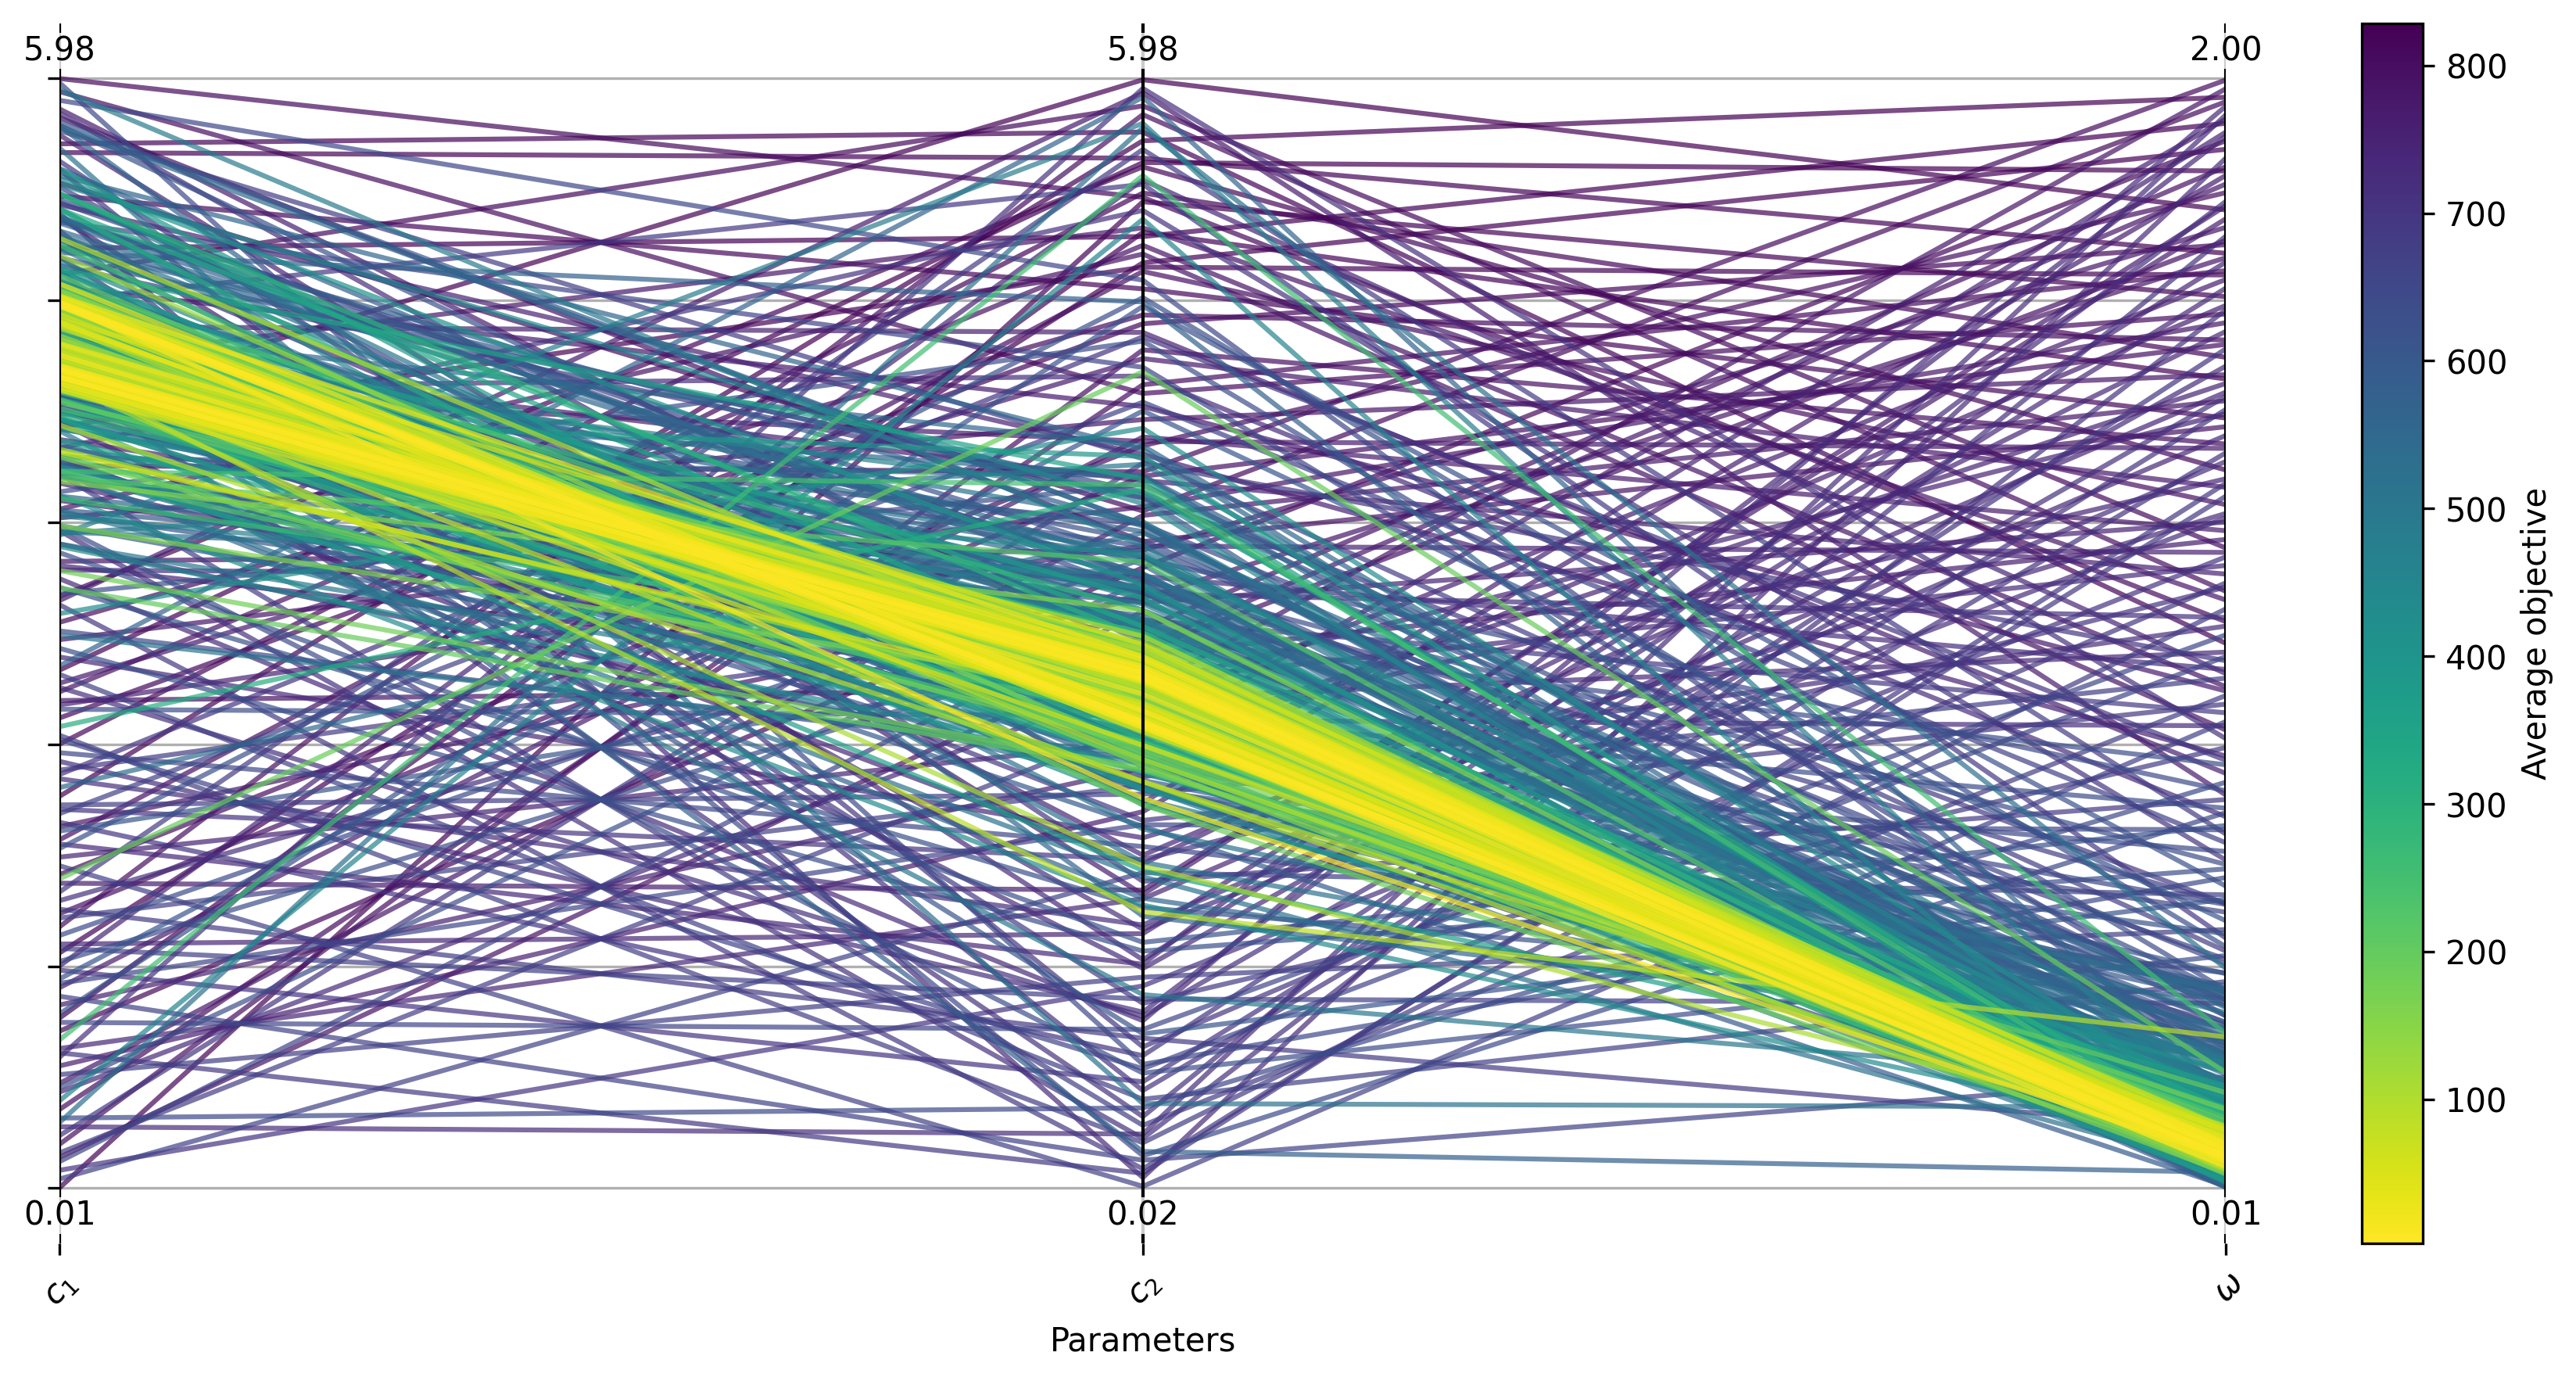
\includegraphics[width=1\textwidth]{Figures/tuning_plots/Parallel_coordinates_plot_for_PSO_parameters.png}
        \caption{PSO}
    \end{subfigure}
    % \hspace{.5cm} % Adjust the space as needed.
    \begin{subfigure}{0.49\textwidth}
        \centering
        \includegraphics[width=1\textwidth]{Figures/tuning_plots/Parallel_coordinates_plot_for_PerturbationPSO_parameters.png}
        \caption{PerturbationPSO}\label{fig:perturbation_params}
    \end{subfigure}
    \begin{subfigure}{0.49\textwidth}
        \centering
        \includegraphics[width=1\textwidth]{Figures/tuning_plots/Parallel_coordinates_plot_for_RebelPSO_parameters.png}
        \caption{RebelPSO}
    \end{subfigure}
    % \hspace{.5cm} % Adjust the space as needed.
    \begin{subfigure}{0.49\textwidth}
        \centering
        \includegraphics[width=1\textwidth]{Figures/tuning_plots/Parallel_coordinates_plot_for_RejectorPSO_parameters.png}
        \caption{RejectorPSO}
    \end{subfigure}
        \begin{subfigure}{0.49\textwidth}
        \centering
        \includegraphics[width=1\textwidth]{Figures/tuning_plots/Parallel_coordinates_plot_for_RebelRejectorPSO_parameters.png}
        \caption{RebelRejectorPSO}
    \end{subfigure}
        \begin{subfigure}{0.49\textwidth}
        \centering
        \includegraphics[width=1\textwidth]{Figures/tuning_plots/Parallel_coordinates_plot_for_ContrarianPSO_parameters.png}
        \caption{ContrarianPSO}
    \end{subfigure}
        \begin{subfigure}{0.49\textwidth}
        \centering
        \includegraphics[width=1\textwidth]{Figures/tuning_plots/Parallel_coordinates_plot_for_DefeatistPSO_parameters.png}
        \caption{DefeatistPSO}
    \end{subfigure}
      \begin{subfigure}{0.49\textwidth}
        \centering
        \includegraphics[width=1\textwidth]{Figures/tuning_plots/Parallel_coordinates_plot_for_ContrarianDefeatistPSO_parameters.png}
        \caption{ContrarianDefeatistPSO}
    \end{subfigure}
        \begin{subfigure}{0.49\textwidth}
        \centering
        \includegraphics[width=1\textwidth]{Figures/tuning_plots/Parallel_coordinates_plot_for_EschewerPSO_parameters.png}
        \caption{EschewerPSO}
    \end{subfigure}
    \begin{subfigure}{0.49\textwidth}
        \centering
        \includegraphics[width=1\textwidth]{Figures/tuning_plots/Parallel_coordinates_plot_for_EscapistPSO_parameters.png}
        \caption{EscapistPSO}
    \end{subfigure}
            \captionsetup{list=no}
\caption[Parallel coordinates plots of parameter configurations]{Parallel coordinates plots showing the distribution of  parameter configurations, colored by their average objective value.}
\end{figure}


\begin{figure}[H]\ContinuedFloat
    \centering
    \begin{subfigure}{0.49\textwidth}
        \centering
        \includegraphics[width=1\textwidth]{Figures/tuning_plots/Parallel_coordinates_plot_for_EschewerEscapistPSO_parameters.png}
        \caption{EschewerEscapistPSO}
    \end{subfigure}
    % \hspace{.5cm} % Adjust the space as needed.
    \begin{subfigure}{0.49\textwidth}
        \centering
        \includegraphics[width=1\textwidth]{Figures/tuning_plots/Parallel_coordinates_plot_for_HybridFullDisjointPSO_parameters.png}
        \caption{HybridFullDisjointPSO}
    \end{subfigure}
    \begin{subfigure}{0.49\textwidth}
        \centering
        \includegraphics[width=1\textwidth]{Figures/tuning_plots/Parallel_coordinates_plot_for_HybridPartialDisjointPSO_parameters.png}
        \caption{HybridPartialDisjointPSO}
    \end{subfigure}
    % \hspace{.5cm} % Adjust the space as needed.
    \begin{subfigure}{0.49\textwidth}
        \centering
        \includegraphics[width=1\textwidth]{Figures/tuning_plots/Parallel_coordinates_plot_for_HybridAdditivePSO_parameters.png}
        \caption{HybridAdditivePSO}
    \end{subfigure}
\caption[Parallel coordinates plots of parameter configurations]{Parallel coordinates plots showing the distribution of  parameter configurations, colored by their average objective value.}
\label{fig:parameter_plots}
\end{figure}

%%% Annexes: Work that *YOU DID NOT* Develop %%%
\ifthenelse{\equal{\LanguageOption}{portuguese}}{
    \addtocontents{toc}{\protect\contentsline{chapter}{Anexos}{}{}}
}{
    \addtocontents{toc}{\protect\contentsline{chapter}{Annexes}{}{}}
}

\setcounter{chapter}{11} % To start at the "L" chapter.
\MediaOptionLogicAnnexes
\begin{center}
    \crimsonfont
    \thispagestyle{empty}
        
    \vspace*{\fill}
    \ifthenelse{\equal{\LanguageOption}{portuguese}}{%
        {\LARGE\fontsize{26}{26}\selectfont\textcolor{maincolor}{Anexos}\par}
    }{%
        {\LARGE\fontsize{26}{26}\selectfont\textcolor{maincolor}{Annexes}\par}
    }
    \vspace*{\fill}
\end{center}
\MediaOptionLogicBlank
\chapter{Showcasing the First Annex}
\guideinfo{Annexes are supplementary sections in a dissertation that provide additional information or external documents not essential to the main arguments but that support or complement the research. Unlike appendices, \textbf{annexes generally contain material that was not developed by the author}, such as reports, legal documents, or published datasets from external sources. This information is placed separately to keep the main content concise, allowing readers access to relevant external references without disrupting the dissertation's flow.}

%%% Back Page %%%
\ifthenelse{\equal{\MediaOption}{paper}}{\blankpage}{}

\clearpage
\null
\thispagestyle{empty}

\ifthenelse{\equal{\CoverOption}{classic}}{
    \newcommand\BackgroundPicBackPage{%
    \put(0,0){%
    \parbox[b][\paperheight]{\paperwidth}{%
    \vfill
    \centering
    \includegraphics[width=\paperwidth,height=\paperheight,keepaspectratio]{Figures/Theme/Cover-BG-dark.pdf}%
    \vfill
    }}}
}{
    \newcommand\BackgroundPicBackPage{%
    \put(0,0){%
    \parbox[b][\paperheight]{\paperwidth}{%
    \vfill
    \centering
    \includegraphics[width=\paperwidth,height=\paperheight,keepaspectratio]{Figures/Theme/Back-Page-BG-W.pdf}%
    \vfill
    }}}
}

\AddToShipoutPictureBG*{\BackgroundPicBackPage}

\newgeometry{margin=1.98cm, top=1.47cm, bottom=1.47cm}
\noindent\clearpage
\restoregeometry

\end{document}